%
% main.tex
%
% Copyright (C) 2023 UFSC.
%
% DOCUMENTATION-TEMPLATE
%
% This work is licensed under the Creative Commons Attribution-ShareAlike 4.0
% International License. To view a copy of this license,
% visit http://creativecommons.org/licenses/by-sa/4.0/.
%

\documentclass[a4paper,12pt]{book}
\usepackage{minted}
\usepackage[most]{tcolorbox}
\usepackage{adjustbox}
\usepackage[ddmmyyyy]{datetime}
\usepackage{lipsum}
\usepackage{book}
\usepackage{datetime}
\newdateformat{monthyeardate}{%
  \monthname[\THEMONTH], \THEYEAR}

\title{RISC-V: An approach for learning the architecture}
\author{SpaceLab}
\date{\today}

% File metadata
\hypersetup
{
  pdfauthor   = {SpaceLab},
  pdfsubject  = {\thetitle},
  pdftitle    = {\thetitle},
  pdfkeywords = {Nanosatellites, CubeSats},
  colorlinks=true,
  urlcolor=blue,
  linkcolor=blue,
  citecolor=black
  }

\usepackage{soul}

\sethlcolor{lightgray}
\usepackage[framemethod=tikz]{mdframed}

\surroundwithmdframed[
  hidealllines=true,
  backgroundcolor=lightgray,
  innerleftmargin=15pt,
  innertopmargin=0pt,
  innerbottommargin=0pt]{lstlisting}

\begin{document}

    \pagenumbering{roman}
    \setcounter{page}{1}

    %
% titlepage.tex
%
% Copyright (C) 2023 UFSC.
%
% DOCUMENTATION-TEMPLATE
%
% This work is licensed under the Creative Commons Attribution-ShareAlike 4.0
% International License. To view a copy of this license,
% visit http://creativecommons.org/licenses/by-sa/4.0/.
%

\begin{titlepage}

\thispagestyle{empty}

\begin{flushleft}
\end{flushleft}

\vspace{1cm}

\begin{figure}[!ht]
    \begin{flushleft}
        
\includegraphics[width=7cm]{figures/horizontal_fundo_claro.png}
    \end{flushleft}
\end{figure}

\begin{flushleft}
\Huge{\textbf{\thetitle}}
\rule[0pt]{\textwidth}{5pt}
\end{flushleft}

\vspace{0.2cm}

\begin{flushleft}
\textit{\thetitle} \\
\textit{Universidade Federal de Santa Catarina, Florianópolis - Brazil}
\end{flushleft}

\vfill
\vfill

\begin{flushright}
\monthyeardate\today
\end{flushright}

\end{titlepage}

    \cleardoublepage
    %
% authorpage.tex
%
% Copyright (C) 2023 UFSC.
%
% DOCUMENTATION-TEMPLATE
%
% This work is licensed under the Creative Commons Attribution-ShareAlike 4.0
% International License. To view a copy of this license,
% visit http://creativecommons.org/licenses/by-sa/4.0/.
%

\thispagestyle{empty}

\begin{center}

\textbf{\thetitle}

\monthyeardate\today

\vspace{1cm}

\textbf{Project Chief:}

Eduardo Augusto Bezerra <\href{mailto:eduardo.bezerra@spacelab.ufsc.br}{eduardo.bezerra@spacelab.ufsc.br}>

\vspace{1cm}

\textbf{Authors:}

João Cláudio Elsen Barcellos <\href{mailto:joaoclaudiobarcellos@gmail.com}{joaoclaudiobarcellos@gmail.com}> \\
Rebecca Quintino Do Ó <\href{mailto:rebeccaqquintino@gmail.com}{rebeccaqquintino@gmail.com}>\\
Yunior Alcantra Guevara <\href{mailto:yunior.alcantara@posgrad.ufsc.br}{yunior.alcantara@posgrad.ufsc.br}>\\

\vspace{1cm}

\textbf{Contributing Authors:}

Alysson Jose Mendes Borba <\href{mailto:alyssonjmb@gmail.com}{alyssonjmb@gmail.com}>\\
Felipe Costa Juliano <\href{mailto:colkiese171@gmail.com}{colkiese171@gmail.com}>\\
%CONTRIBUTING AUTHOR 3 \\

\vspace{1cm}


\textbf{Revision Control:}


\begin{table}[!ht]
    \begin{center}
        \begin{tabular}{cL{4cm}L{4cm}C{2cm}}
            \toprule[1.5pt]
            \textbf{Version} & \quad\quad\quad \textbf{Author}  & \quad\quad \textbf{Changes} & \textbf{Date} \\
            \midrule
            1.0 & J. C. E. Barcellos, Rebecca Q. Do Ó and Y. A. 
            Guevara & Document creation & 2023/05/10 \\
            \bottomrule[1.5pt]
        \end{tabular}
    \end{center}
\end{table}

\textbf{Contributions:}

\begin{table}[!ht]
    \centering
    \begin{tabular}{cL{5cm}L{5.5cm}C{2cm}}
        \toprule[1.5pt]
        \textbf{Author} & \quad\quad\quad \textbf{Chapters}\\
        \midrule
        J. C. E. Barcellos & \quad\quad 4, 5, 6, 7, 8 and 9\\
        Rebecca Q. Do Ó    & \quad\quad 2, 3, 4, 6 and 9\\
        Y. A. Guevara      & \quad\quad 1, 2, 3, 6, 7 and 9\\
        \bottomrule[1.5pt]
    \end{tabular}
\end{table}
\end{center}

\vspace{1cm}

\begin{figure}[!h]
	\begin{center}
		
\includegraphics[width=0.25\textwidth]{by-sa.pdf}
	\end{center}
\end{figure}

\textcopyright\  2023 by UFSC. \thetitle. This work is licensed under the Creative Commons Attribution-ShareAlike 4.0 International License. To view a copy of this license, visit \href{http://creativecommons.org/licenses/by-sa/4.0/}{http://creativecommons.org/licenses/by-sa/4.0/}.


    \cleardoublepage

    \listoffigures
    \addcontentsline{toc}{chapter}{List of Figures}

    \listoftables
    \addcontentsline{toc}{chapter}{List of Tables}

    \printnomenclature
    \addcontentsline{toc}{chapter}{Nomenclature}

    \tableofcontents
    \cleardoublepage
    
    \pagenumbering{arabic}
    \setcounter{page}{1}

    \chapter{Introduction}

RISC-V is an open-source instruction set architecture (ISA) designed for computer processors. It stands for ``Reduced Instruction Set Computing - Version 5.0''. RISC-V is different from proprietary ISAs like x86 (Intel) or ARM because it is an open standard that can be freely used, modified, and implemented by anyone without requiring license fees or restrictions.

The RISC-V ISA is based on a simple, modular, and extensible design philosophy. It aims to provide a flexible foundation for a wide range of computing devices, from small embedded systems to large-scale servers. The instruction set is designed to be efficient, easy to understand, and conducive to efficient hardware implementation.

RISC-V supports several standard extensions, which provide additional functionality beyond the base instruction set. These extensions include integer multiplication and division, floating-point arithmetic, atomic memory operations, vector processing (SIMD), and more. The modular nature of RISC-V allows implementers to choose the extensions that best suit their specific requirements.

One of the key advantages of RISC-V is its open nature. It enables academic researchers, industry professionals, and hobbyists to contribute to the development and improvement of the architecture. This openness has led to a growing ecosystem around RISC-V, including a wide range of compatible processors, development boards, software tools, and libraries.

RISC-V has gained significant attention and adoption in recent years, particularly in areas such as Internet of Things (IoT), embedded systems, and academic research. It has also seen interest from industry giants like NVIDIA, Western Digital, and SiFive, who have developed RISC-V-based products or contributed to the development of the ecosystem.

In this document, different aspects of RiSC-V are studied, dividing the document into chapters. In \autoref{ch:chapter_riscv_prof}, the RISC-V architecture is analyzed and explained, explaining each block and the operation of the pipeline, as well as a brief analysis of the set of instructions. In \autoref{ch:chapter_riscv_stud}, the RISC-V is explained in a simple and concise way to make it easier for beginning students to understand. Then, in \autoref{chp:chapter_cl}, an introduction to the C language is made using a micro-controller with RISC-V architecture, where some examples are presented. In \autoref{chp:chapter_s} a representation of the memory allocation mode used by NEORV32 is made. Then, in \autoref{chp:chapter_p}, the peripherals of the microprocessor based on RISC-V NEORV32 are presented. In \autoref{chp:chapter_rec}, the procedure for configuring the FPGA to operate with NEORV32 and how to install the toolchain is explained. Then, in \autoref{ch:chapter_comp} the first compilation and execution of a program is made using the presented setup. Finally, in \autoref{chp:chapter_ex}, more advanced examples are presented in C language using the RISC-V architecture.



 % presents the book
    %
% introduction.tex
%
% Copyright (C) 2023 UFSC.
%
% DOCUMENTATION-TEMPLATE
%
% This work is licensed under the Creative Commons Attribution-ShareAlike 4.0
% International License. To view a copy of this license,
% visit http://creativecommons.org/licenses/by-sa/4.0/.
%
% aluno
% 1 - risc-v: intructions architectures. nao precisa colocar como as instruções são executadas (pipeline). colocar os registradores. colocar imagens mais simples da arquitetura do risc-v. diferença de microprocessador e microntrolador.
% 2 - mostra a cpu  e os perifericos, so que nao na primeira aula. na primeira aula so CPU e os registradores. o que é o mapeamento de memória? o que acontece nos registradores? 
% 2-3 agrupar conforme as aulas do 8051.
% 4 - aprensentar no inicio do documento
% 5 - deixa onde estar

% professor
% 1 - pipeline, risc-v instructions
% 3.2 - livro do técnico

\chapter{RISC-V} \label{ch:chapter_riscv_prof}

Welcome to \autoref{ch:chapter_riscv_prof}, dedicated to analyzing and explaining the RISC-V architecture, explaining each block and the operation of the pipeline, as well as a brief look at the instruction set.

The following sections will provide a comprehensive overview of the fundamental components of a RISC-V architecture processor.

\autoref{sec:section_riscv_prof.1}:
    In this subsection, we will cover the basic topics about RISC-V architecture, comprising the combinational elements, the sequential elements, the clocking methodology, instruction lookup, instruction types, and the composition of the elements.
    
\autoref{sec:section_riscv_prof.2}:
In this subsection, we will talk about the RISC-V architecture, understanding its aspects of operation such as an overview of the CPU, multiplexers, control, datapath, the instruction types, ALU control, central control unit and pipeline including hazards.

\autoref{sec:section_riscv_prof.3}:
Finally, in this section we will cover about the instructions, understanding their operation with assembly.

    \section{RISC-V Basics} \label{sec:section_riscv_prof.1}
    
    In RISC-V the information is encoded in binary, where low voltage represents 0 and high voltage represents 1. Each bit of information is typically transmitted over a single wire, with multiple bits forming multi-bit data transmitted over multi-wire buses.

        \subsection{Combinational Elements} 
        
        Combinational elements operate on data by performing specific operations or transformations. These elements take input signals and produce output signals based on a defined logic function. The output is solely determined by the current input values and does not depend on any previous state or history.
        
        \subsection{Sequential Elements}
        
         Sequential elements or state elements, are used to store information and introduce memory into the system. They maintain a state that can change over time based on the inputs and the current state. Sequential elements, such as flip-flops or registers, store and remember information, allowing for sequential and memory-dependent operations.
        
        \subsection{Clocking Methodology}
        
        The clocking methodology used in RISC-V processors follows a synchronous clocking approach. In RISC-V, a central clock signal is generated and distributed to all the components within the processor. The clock signal acts as a reference for the timing of instructions execution and synchronization of various operations.
        
        \subsection{Instruction Fetch}
        
        Instruction Fetch, also known as the fetch stage, is a step in the execution cycle of a RISC-V processor. In this stage, the processor retrieves the next instruction to be executed from memory.
        
        \subsection{R-Format Instructions}
        
        R-Format instructions in the RISC-V architecture are instructions that operate on registers. They have a fixed 32-bit structure with specific fields for the operation type, source and destination registers, and additional function bits. These instructions perform arithmetic, logical, and data manipulation operations by using the values in the source registers and storing the result in the destination register. They provide flexibility and efficiency by allowing direct register-to-register operations, making them essential for data processing in the RISC-V architecture.
        
        \subsection{Load/Store Instructions}
        
        Load/Store instructions in the RISC-V architecture facilitate the transfer of data between registers and memory. Load instructions retrieve data from memory and store it in a register, while store instructions take data from a register and store it in memory. These instructions are essential for data manipulation and memory access in RISC-V programs, enabling efficient reading from and writing to memory locations.
        
        \subsection{Branch Instructions}
        
        Branch instructions in the RISC-V architecture are used for conditional branching, allowing programs to alter the flow of execution based on certain conditions. These instructions compare values in registers and determine whether to branch to a different instruction or continue sequentially. Branch instructions are essential for implementing control flow, such as loops and conditional statements, in RISC-V programs. They enable program execution to make decisions and follow different paths based on the evaluated conditions, enhancing the flexibility and versatility of the architecture.
        
        \subsection{Composing the Elements}
        
        Composing the elements in the RISC-V architecture involves combining different components to create a functional system. This includes integrating the CPU core, memory subsystem, input/output interfaces, and other peripherals. The elements are interconnected through buses or interconnects, enabling communication and data transfer between them. The composition of these elements requires careful design and consideration to ensure proper functionality and performance of the RISC-V system as a whole.

    \section{RISC-V Architecture} \label{sec:section_riscv_prof.2}
    
    The RISC-V architecture will be studied in the following subsections. The idea is to start with a simplified diagram of the processor and gradually add architecture blocks.

        \subsection{CPU Overview}
        
        A RISC-V CPU (Central Processing Unit) is the central component of a computer system that executes instructions based on the RISC-V instruction set architecture. The CPU fetches instructions from memory using the Program Counter (PC) and decodes them to determine the operation and involved operands. Next, the CPU executes the instruction by performing the arithmetic, logical, memory access, or control flow operations specified by the instruction and updates registers or memory \cite{patterson}.
        
                \begin{figure}[!h]
        	    \centering
        	    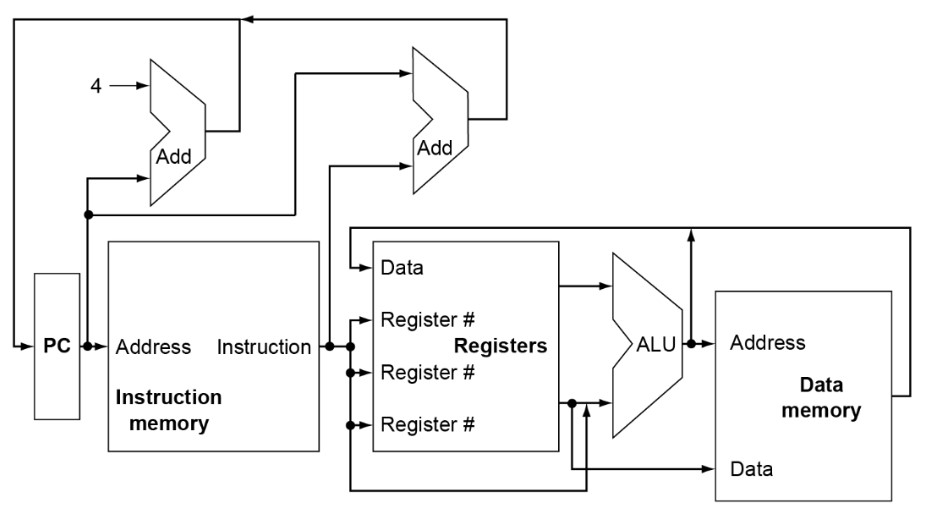
\includegraphics[width= 0.7
        	    \textwidth]{figures/riscv/risc_1.jpg}
                    \caption{\label{risc_1} CPU Overview Diagram}
                \end{figure}
        
        Figure \ref{risc_1} show an overview of the key components of the RISC-V CPU, where ``PC'' is the program counter, an 32-bit or 64-bit register; the ``Add'' are adders; ``Instruction Memory'' refers to the component of the processor that stores and provides the instructions to be executed by the processor; ``Registers'' are small storage units within the processor that hold data and instructions during program execution. They are used for fast and efficient data manipulation, storing intermediate values, and holding the results of computations; ``ALU'' is the arithmetic logic unit; and ``Data memory'' is the part of the processor that stores and retrieves data during program execution. It provides a space for reading and writing data, allowing the processor to access and manipulate variables, arrays, and other data structures required by the program. 
        
        
        \subsection{Multiplexers}
        
        Multiplexers (MUX), are critical components used for selecting one of several inputs to be passed as the output. This components play a significant role in data routing and control signal selection within the CPU, for example, in the Figure \ref{risc_1a} it is necessary to put an MUX in each red circle, as it is not possible to simply join the wires.
        
                \begin{figure}[!t]
        	    \centering
        	    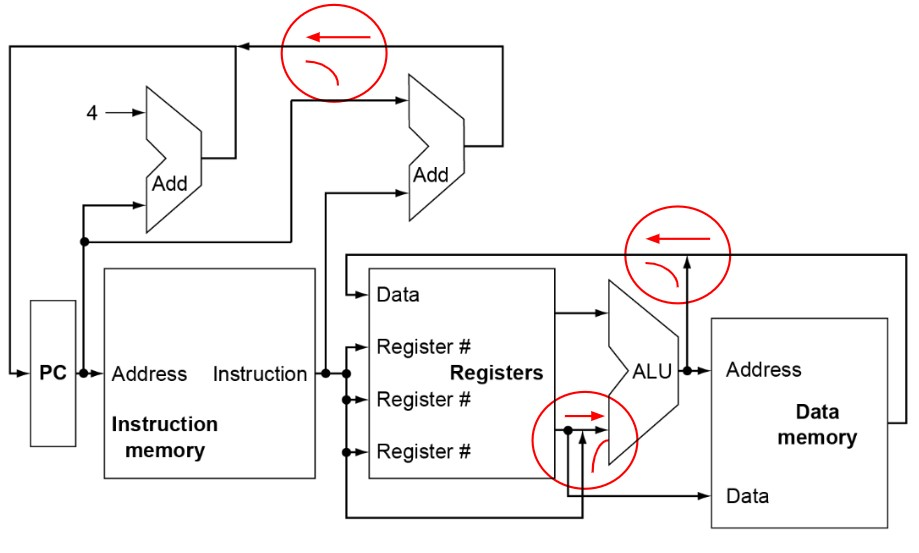
\includegraphics[width= 0.7
        	    \textwidth]{figures/riscv/risc_1a.jpg}
                    \caption{\label{risc_1a} Diagram showing where multiplexers are needed}
                \end{figure}
        
        \subsection{Control}
        
        Control in RISC-V architecture is responsible for decoding instructions, generating the necessary control signals, and coordinating the execution of operations within the CPU. The control unit determines which components should be activated or deactivated, such as the ALU, registers, and multiplexers, to perform the operations specified by the instructions.
        
                \begin{figure}[!h]
        	    \centering
        	    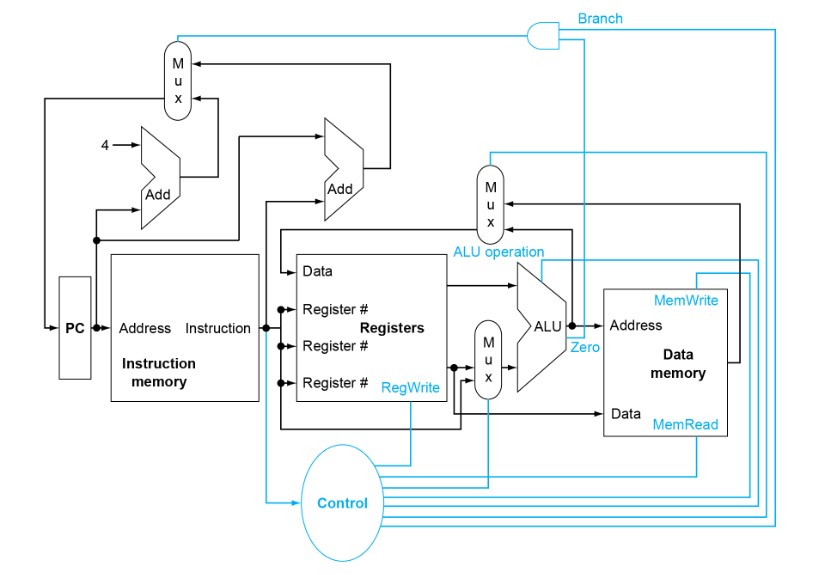
\includegraphics[width= 0.8
        	    \textwidth]{figures/riscv/risc_2.jpg}
                    \caption{\label{risc_2} Diagram with added control signals}
                \end{figure}
                
        Figure \ref{risc_2} shows the control unit and its connections in blue. At this first moment, the control is only used in ``RegWrite'', indicating if the result of an instruction must be written back in a register; ``MemRead'' and ``MemWrite'' to indicate whether a memory read or write operation should be performed; ``Branch'' used for implementing conditional branching or jump operations. In control, the ``ALUOperation'' signal can have different values, each corresponding to a specific operation that the ALU should perform. Some common examples of operations controlled by ``ALUOp'' include addition, subtraction, logical operations (AND, OR, XOR), bit shifting, and comparisons. Finally, the ``Zero'' control signal refers to a flag or signal that indicates whether the result of an operation performed by the ALU is equal to zero. This flag is used to make conditional decisions based on the result of a previous operation.

        \subsection{Full Datapath}

            In Figure \ref{risc_4} you can see the full RISC-V Diagram, where all the blocks that have been added sequentially are present. 
            
                    \begin{figure}[!h]
            	    \centering
            	    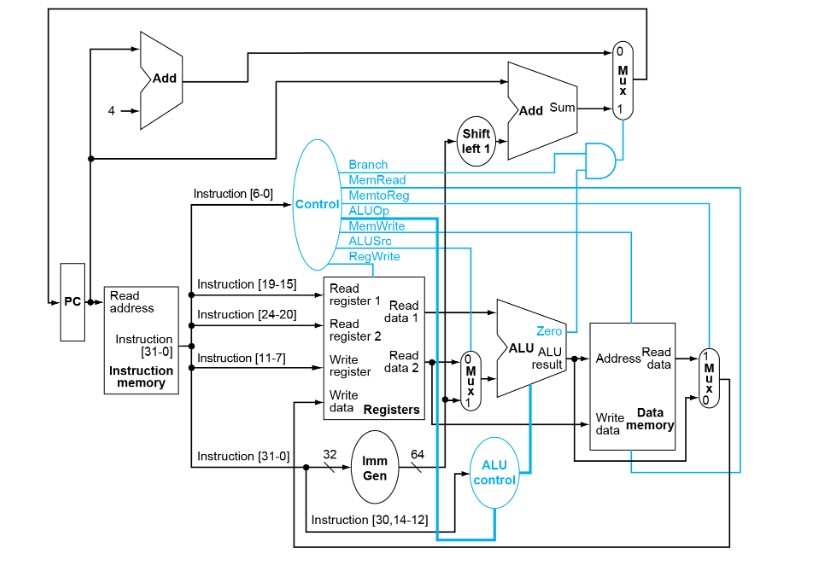
\includegraphics[width= 1
            	    \textwidth]{figures/riscv/risc_4.jpg}
                        \caption{\label{risc_4} RISC-V Full Datapath}
                    \end{figure}
            In the diagram, the specific bits of an instruction are routed to the different control blocks and functional units of the processor as follows:
    
            \begin{itemize}
            \item Bits [6-0] are connected to the control block. These bits are used to determine the specific operation that the instruction will perform.
            \item Bits [19-15] are used to select the read register 1. These bits indicate which register will be read to provide one of the operands for the operation.
    
            \item Bits [24-20] are used to select the read register 2. These bits indicate which register will be read to provide the second operand for the operation.
    
            \item Bits [11-7] are used to select the write register. These bits indicate in which register the result of the operation will be stored.
    
            \item Bits [31-0] are directed to the ``Imm Gen'' (Immediate Generation) block. These bits are used to generate the immediate value required by the instruction.
    
            \item Bits [30, 14-12] are used to control the control block of the Arithmetic Logic Unit (ALU). These bits determine the specific operation that the ALU will perform.
            \end{itemize}
        
        \subsection{R-Type/Load/Store Datapath}

            \begin{figure}[!h]
            \centering
            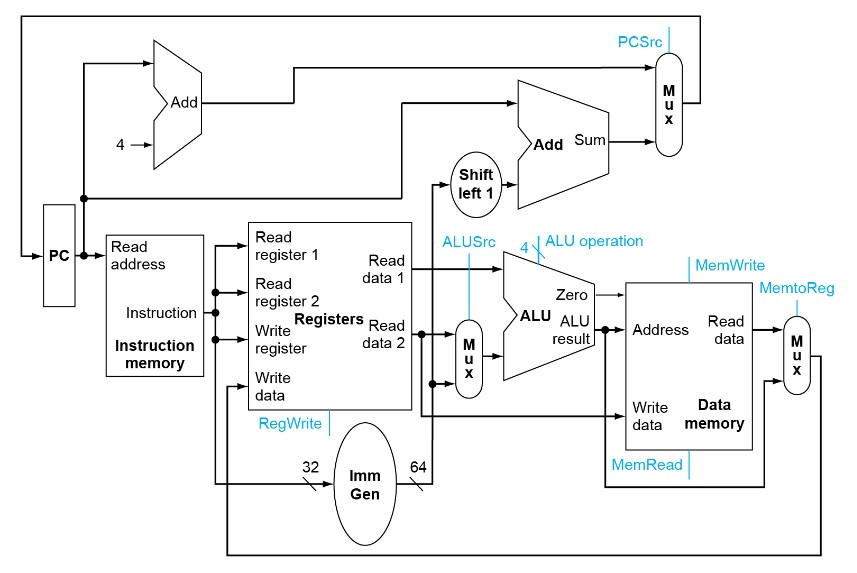
\includegraphics[width = 0.8
            \textwidth]{figures/riscv/risc_3.jpg}
                \caption{\label{risc_3} Diagram with added R-Type/Load/Store signals}
            \end{figure}

            At this time the R-Type, Load and Store instructions in the Diagram are added (Figure \ref{risc_3}). In the representation, ``ALU Src'' (ALU Source) is a control signal that determines the input data source to the Arithmetic Logic Unit (ALU) during the execution of an instruction. Specifically, the ALU Src signal determines whether the input value to the ALU will come from a register or an immediate value; ``PC Src'' (PC Source) in RISC-V is a control signal that determines the data source used to update the value of the PC during the instruction fetch cycle; ``MemToReg'' (Memory to Register) is a control signal in the RISC-V architecture that determines whether the data loaded from memory should be written back to a register in an instruction execution cycle; and ``Imm Gen'' (Immediate Generation) is a unit responsible for generating the immediate value used in instructions that involve operations with constant values embedded within the instruction itself.
    
            Shown below are three examples of the processor and Datapath with Control parts used in three different types of R-Type, Load, and BEQ instructions. 
        
            \subsubsection{R-Type Instruction}
        
                \begin{figure}[!h]
                \centering
                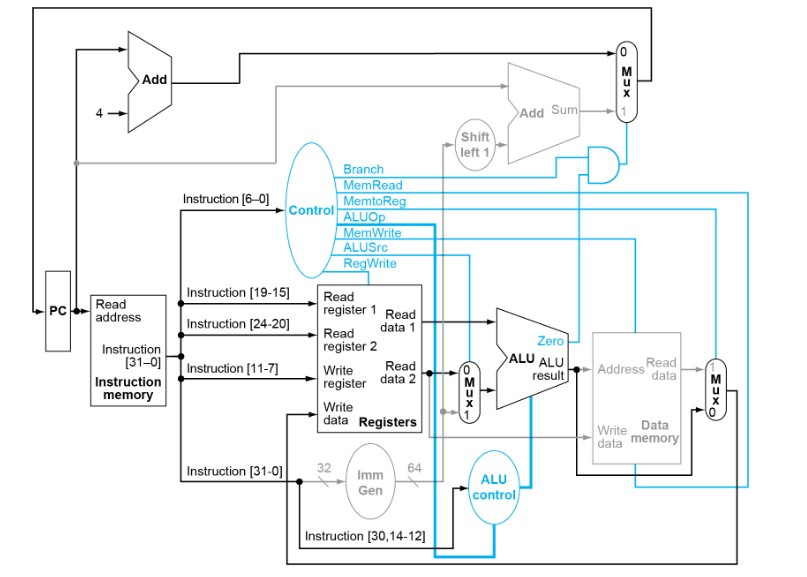
\includegraphics[width= 0.8
                \textwidth]{figures/riscv/risc_R-type.jpg}
                    \caption{\label{risc_R-type} RISC-V R-Type}
                \end{figure}
                
                Figure \ref{risc_R-type} shows the processor diagram executing an R-Type instruction. The gray parts represent the parts of the processor that are not being used and the blue parts represent the control part. In this instruction, the Imm Gem blocks are not used and values are not written to the memory, as well as the PC receives an increase of four units.  In this format, the instruction has three registers as operands and a destination register where the result will be stored. The operations supported by the R-type format include addition, subtraction, multiplication, division, logical operations (AND, OR, XOR), and shifting. The R-type instruction is widely used to perform calculations and data manipulations within the RISC-V processor.
            
            \subsubsection{Load Instruction}

                \begin{figure}[!h]
                \centering
                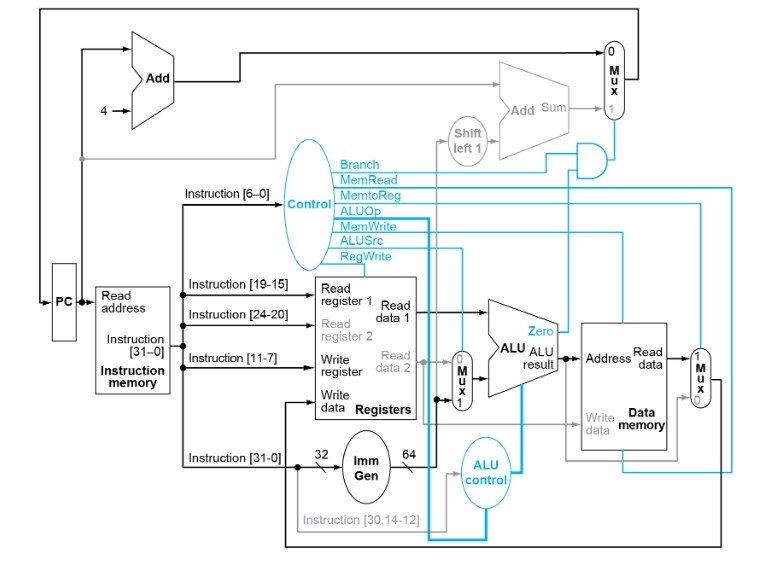
\includegraphics[width= 0.8
                \textwidth]{figures/riscv/risc_L-type.jpg}
                    \caption{\label{risc_L-type} RISC-V Load Instruction}
                \end{figure}

                On the other hand, Figure \ref{risc_L-type} shows a Load instruction being executed. Note that in this instruction only Imm Gen is used, and memory values are read. The Load instruction in RISC-V is used to fetch a value from memory and load it into a specific register. It allows the processor to access and use data stored in memory. The Load instruction typically requires specifying the memory address from where the data should be fetched and the destination register where the data will be stored. It is an essential instruction for reading data from memory and is used in various data processing operations, such as accessing array elements, reading variables, or retrieving data from external devices.
            
            \subsubsection{BEQ Instruction}

                \begin{figure}[!h]
                \centering
                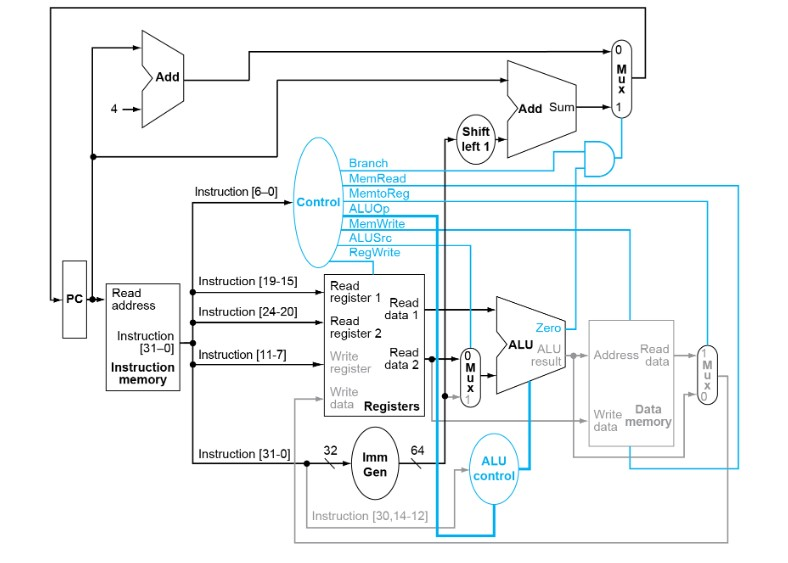
\includegraphics[width= 0.8
                \textwidth]{figures/riscv/risc_BEQ-type.jpg}
                    \caption{\label{risc_BEQ-type} RISC-V BEQ Instruction}
                \end{figure}

                In the case of Figure \ref{risc_BEQ-type} a BEQ (Branch if Equal) instruction is presented. This type of instruction does not access memory, is a conditional branch instruction that checks if two registers are equal and performs a branch to a specified address if the condition is true. It is used to control the flow of program execution based on equality comparisons between register values. The BEQ instruction is used to implement conditional control structures such as loops and decision structures, allowing the program to take different execution paths based on the specified conditions.                

       \subsection{ALU Control}

            The ALU (Arithmetic Logic Unit) control in RISC-V is responsible for determining the operation to be performed by the ALU based on the instruction. It decodes the relevant fields of the instruction and generates control signals to configure the ALU accordingly. This enables the ALU to execute arithmetic, logical, and bitwise operations as specified, contributing to data processing in the RISC-V processor.
        
        
       \subsection{The Main Control Unit}

            The Main Control Unit controls the data flow between the memory, instruction register, data register, ALU, and other elements of the processor. It ensures that instructions are executed correctly by coordinating memory access, instruction fetching and decoding, and data manipulation.
            
            Moreover, the Main Control Unit implements the control logic that determines the next state of the processor based on the current instruction. This includes selecting the next instruction address, controlling registers, and generating the appropriate control signals for each component of the processor.
            
        \subsection{RISC-V Pipeline}
            
            The RISC-V architecture supports a five-stage pipeline known as the RISC-V pipeline. The five stages of the pipeline are:
            \begin{enumerate}
            \item Instruction Fetch (IF): In this stage, the processor fetches the instruction from memory. The program counter (PC) is used to fetch the instruction from the memory address pointed to by the PC.
            \item Instruction Decode (ID): In this stage, the fetched instruction is decoded, and the necessary control signals and register operands are prepared for the subsequent stages. The register operands are read from the register file, and immediate values are sign-extended if needed.
            \item Execute (EX): In this stage, the ALU (Arithmetic Logic Unit) performs the arithmetic or logical operation specified by the instruction. This stage also handles branch and jump instructions, where the target address is computed.
            \item Memory Access (MEM): In this stage, memory operations such as load and store are performed. For load instructions, the memory is accessed to retrieve the required data, while store instructions write data from a register to the memory.
            \item Write Back (WB): In this final stage, the results of the executed instruction are written back to the register file. This includes the result of ALU operations or the data loaded from memory.
            
            \end{enumerate}
            
            Implementing a pipeline in RISC-V can significantly increase processor performance. Similar to the example in Figure \ref{pipe2}, pipeline divides instruction processing into sequential stages, allowing multiple instructions to be executed in parallel and speeding up the processing rate.
            
            \begin{figure}[!h]
            \centering
            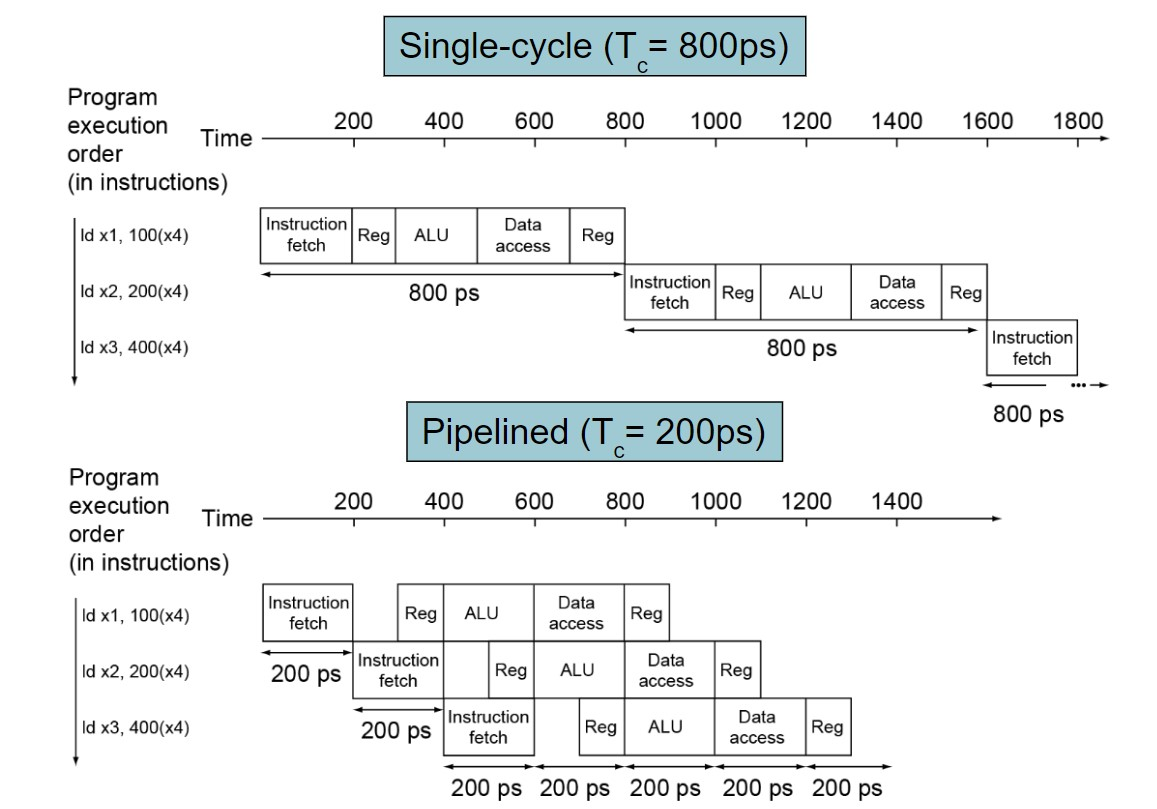
\includegraphics[width=0.8\textwidth]{figures/riscv/pipe2.jpg}
                \caption{\label{pipe2} Pipeline performance representation }
            \end{figure}

    
            \subsubsection{Hazards}

                Hazards are situations where the correct and efficient execution of instructions is hindered due to data dependencies or the sequential nature of instructions. Hazards can result in pipeline delays, reducing the performance of the processor. There are three main types of hazards in RISC-V:

                \begin{itemize}

                \item Data Hazard: Occurs when an instruction depends on a result produced by a previous instruction that has not yet completed. This can occur in cases of reading a value that has not been written yet or writing to a register before its value is read by subsequent instructions.

                \item Control Hazard: Occurs when a conditional branch instruction alters the normal flow of program execution. This can result in uncertainty about which instruction will be executed next, causing delays in instruction fetch and forwarding of subsequent instructions.
                
                \item Structural Hazard: Occurs when there is a conflict in physical resources of the processor, such as functional units, memory, or registers. This can occur when two instructions need to access the same resource simultaneously, resulting in delays and potentially requiring instruction reordering.
                \end{itemize}
                
                To deal with hazards in RISC-V, various techniques can be applied, such as data forwarding, instruction scheduling, branch prediction, and the use of buffers to avoid structural conflicts.

    \section{RISC-V Instructions} \label{sec:section_riscv_prof.3}

        \subsection{Arithmetic instructions use register
        operands}
        
            In RISC-V, there are 32 general-purpose registers, labeled from x0 to x31. These registers are 64 bits wide and can hold data or addresses.
            
            Here is a brief overview of the common uses and conventions for some of the registers in RISC-V:
            
            x0 (zero register): This register is hardwired to the constant value zero and cannot be modified. It is often used for special purposes such as encoding a constant zero value or serving as a destination for instructions that discard their results.
            
            x1 (ra, return address): This register is typically used to store the return address when executing function calls. It is usually automatically managed by the function calling convention.
            
            x2 to x7 (a0 to a7, argument registers): These registers are commonly used to pass function arguments. The first few arguments to a function are typically placed in these registers according to the function calling convention.
            
            x8 (t0 to t2, temporary registers): These registers are often used as temporary storage during computations within a function. They are not required to be preserved across function calls.
            
            x9 (s0/fp, saved register/frame pointer): This register is usually used as a frame pointer or base pointer for accessing local variables and parameters within a function. It may also be used as a general-purpose register.
            
            x10 to x17 (s1 to s8, saved registers): These registers are commonly used for saving and restoring values across function calls. They are expected to be preserved by callee functions.
            
            x18 to x27 (t3 to t4, temporary registers): Similar to x8, these registers are used as temporary storage during computations. They are not required to be preserved across function calls.
            
            x28 to x31 (gp, tp, and other special registers): These registers are reserved for special purposes, such as the global pointer (gp) and the thread pointer (tp). They may also be used for platform-specific purposes.
            
            It's important to note that the specific usage and conventions for registers may vary depending on the compiler, calling convention, and programming context. Additionally, RISC-V supports extensions that introduce additional registers beyond the base set of 32 registers.\\
            Example: \\
            C Code \\
            f = (g + h) - (i + j); \\
            f, …, j in x19, x20, …, x23 \\
            \\
            Compiled RISC-V code: \\
            add x5, x20, x21\\
            add x6, x22, x23\\
            sub x19, x5, x6\\
            
        \subsection{Memory Operands}
            In RISC-V, memory operands are used to access and manipulate data stored in memory. There are different types of memory operands in the RISC-V architecture:
            
            Load: Load instructions are used to read data from memory into registers. They transfer data from memory to a specified register. The general syntax of a load instruction i
            lw rd, offset(rs1)
            Here, ``rd'' is the destination register that will receive the value read from memory, ``offset'' is an immediate value that specifies the offset from the base address (rs1), which is another register used as the base address.
            
            Store: Store instructions are used to write data to specified memory addresses. They transfer data from a register to memory. The general syntax of a store instruction is:
            \begin{center}
            sw rs2, offset(rs1)
            \end{center}
            Here, ``rs2'' is the register that contains the value to be stored in memory, ``offset'' is the offset from the base address (rs1), which is the register used as the base address.
            
            Immediate Addressing: Some instructions allow the use of immediate values as memory operands. These immediate values are added to the base address to calculate the effective memory address. For example:
            \begin{center}
            lw rd, imm(rs1)
            \end{center}
            In this case, ``imm'' is an immediate value that is added to the value in register rs1 to calculate the effective memory address.
            
            These memory operands are used to read and write data in memory during the execution of programs in RISC-V. They enable efficient access to data stored in the main memory, facilitating the implementation of read and write operations in RISC-V programs.
            Example: \\
            C code:\\
            A[12] = h + A[8]; \\
            h in x21, base address of A in x22 \\
            \\
            Compiled RISC-V code: \\
            Index 8 requires offset of 64 8 bytes per double word\\
            ld x9, 64(x22)\\
            add x9, x21, x9\\
            sd x9, 96(x22)\\
        
        \subsection{Immediate Operands}
        
            In RISC-V, immediates are constant values used as operands in instructions. Immediates in RISC-V can have different sizes and formats, depending on the instruction they are used in. 
            
            Here are some common formats of immediates in RISC-V:
            
            I-immediates: These 12-bit immediates are used in load, store, and immediate arithmetic instructions. They can represent immediate integer values from -2048 to 2047.
            
            S-immediates: These 12-bit immediates are used in store instructions, such as SW (store word). They specify the offset from the base address to access memory.
            
            B-immediates: These 13-bit immediates are used in conditional branch instructions, such as BEQ (branch if equal). They represent the offset from the current address to determine the branch target.
            
            U-immediates: These 20-bit immediates are used in immediate load instructions, such as LUI (load upper immediate). They specify the upper 20 bits of a 32-bit value that will be loaded into a register.
            
            J-immediates: These 21-bit immediates are used in unconditional jump instructions, such as JAL (jump and link). They represent the offset from the current address to determine the jump target.
        
        \subsection{Unsigned Binary Integers}
        
            In RISC-V, unsigned binary integers are represented and manipulated without considering the sign of the numbers. This means that they are treated as positive numbers regardless of the sign bit.
            
            Unsigned binary integers in RISC-V are represented in binary notation, where each bit represents a specific value. For example, an 8-bit number can range from 0 to 255, while a 32-bit number can range from 0 to 4,294,967,295.
        
        \subsection{2s-Complement Signed Integers}
        
            In RISC-V, 2's complement is the standard representation used for signed integers. It is a binary representation where the most significant bit (MSB) is used as the sign bit, with 0 indicating a positive number and 1 indicating a negative number.
            
            To represent a negative integer in 2's complement form, the positive value is first represented in binary and then inverted (flipping all the bits), and finally, 1 is added to the result.
            
            For example, let's consider an 8-bit signed integer. To represent -5 using 2's complement:
            
            \begin{enumerate}
            \item Start with the binary representation of 5: 00000101.
            \item Invert all the bits: 11111010.
            \item Add 1 to the result: 11111011.
            \end{enumerate}
            The resulting binary representation, 11111011, represents -5 in 2's complement form.\\
            
            To perform arithmetic operations on 2's complement signed integers, RISC-V instructions handle signed numbers by treating them as regular binary numbers. The signedness of the numbers is determined based on the instruction being executed.
        
        
        \subsection{Signed Negation}
        
            In RISC-V, the negation of a signed integer is typically performed using the negation instruction, which is denoted as ``neg'' or ``negw'' depending on the operand size (32-bit or 64-bit). This instruction changes the sign of the given value.
            
            For example, to negate a signed integer in RISC-V:
            
            Load the signed integer value into a register, let's say register x1.
            Execute the negation instruction, which negates the value in the register:
            neg x1, x1
            After executing this instruction, the value in register x1 will be the negation of the original signed integer.
            
            It's important to note that the negation instruction works based on the 2's complement representation used for signed integers in RISC-V. It flips all the bits of the value and adds 1 to obtain the negated result.
        
        \subsection{Sign Extension}

            Sign extension is an operation used in the RISC-V processor to extend the sign of a smaller-sized binary number to a larger size. It is achieved by replicating the sign bit (Most Significant Bit - MSB) of the smaller number and filling in the additional bits. This sign extension is crucial to preserve the correct negative or positive value during arithmetic operations and comparisons in RISC-V. The sign extension ensures that the sign bit is properly propagated to maintain the integrity and accuracy of calculations performed by the processor.
        
        \subsection{Representing Instructions}

            In RISC-V, instructions are represented as binary codes, with each instruction encoded into a specific bit pattern. The instruction format in RISC-V is fixed-length, meaning that each instruction occupies the same number of bits or 32 bits. This allows for simplified instruction decoding and efficient instruction fetching. The binary representation of instructions includes fields for specifying the operation, source and destination registers, immediate values, and other necessary information for executing the instruction. By following the specific encoding scheme of RISC-V, the processor can accurately interpret and execute the instructions to perform desired operations.        
        
        \subsection{Hexadecimal}

            In RISC-V, instructions can be represented in hexadecimal format, which is a base-16 numbering system. Hexadecimal representation uses the digits from 0 to 9 and the letters from A to F to represent values from 0 to 15. Converting instructions from binary format to hexadecimal format can make them easier to read and communicate. Each hexadecimal digit corresponds to four binary digits, allowing for a more compact representation of instructions. 
        
        \subsection{RISC-V R-format Instructions}

             The R-format instructions have a fixed format with fields for the operation code (opcode), source registers, destination register, and function code. The opcode specifies the operation to be performed, while the source registers provide the operands, and the destination register stores the result. The function code further refines the operation within the opcode category. R-format instructions allow for efficient register-based computations in RISC-V processors.
        
        \subsection{RISC-V I-format Instructions}

            The I-format has fields for the opcode, source register, destination register, and immediate value. The opcode indicates the operation to be performed, the source register provides the register operand, and the immediate value is a constant value or offset used in the operation. I-format instructions enable efficient operations with registers and immediate values in RISC-V processors, such as load/store operations, arithmetic operations, and logical operations with immediate values.
        
        \subsection{RISC-V S-format Instructions}

            The opcode specifies the store operation, the source register provides the data to be stored, the base register holds the memory address, and the immediate value is an offset used to calculate the final memory address. S-format instructions are essential for manipulating data in memory, such as storing values to arrays or updating variables in RISC-V processors.
        
        \subsection{Register Usage}

            The RISC-V architecture provides a set of general-purpose registers that can be used to store operands and instruction results. These registers are directly accessible by the programmer and are used for arithmetic, logical, and control operations.
            
            RISC-V has a total of 32 32-bit registers, numbered from x0 to x31. Among these, register x0 is special and always holds the value zero. Registers x1 to x31 can be used to store temporary values, intermediate results, or memory addresses.
                    
            In addition to general-purpose registers, RISC-V also has special registers such as the program counter (PC), which stores the address of the next instruction to be executed, and the floating-point register (FPU), which handles floating-point operations. 

        \subsection{Memory Layout}
            
            The memory layout is essential for proper program execution and efficient memory management. Here are the common memory regions in RISC-V:
            
            \begin{itemize}
            \item Text Segment: Also known as the code segment, this region is used to store program instructions. It is typically marked as read-only and contains executable code.
            
            \item Data Segment: The data segment contains initialized and uninitialized data used by the program. It is divided into two sub-regions:
            
            \item Initialized Data: This sub-region holds variables and constants with initial values. It includes global variables and static variables.
            
            \item Uninitialized Data (BSS): The BSS (Block Started by Symbol) segment contains uninitialized variables and is initialized with zeros by the system before program execution.
            
            \item Stack: The stack is a memory region used to store local variables, function call information, and return addresses. It grows and shrinks dynamically as functions are called and return.
            
            \item Heap: The heap is a dynamic memory region used for dynamically allocating memory, such as dynamically created objects or data structures. It grows and shrinks based on memory allocation and deallocation requests.
            
            \end{itemize}
            
            The memory layout is usually defined by the linker during the linking process. The program instructions and data are loaded into the appropriate memory regions based on their respective sections in the object file.

        
\chapter{RISC-V for Students} \label{ch:chapter_riscv_stud}
    Welcome to \autoref{ch:chapter_riscv_stud}, this is a version of the RISC-V approach dedicated to students. 
    The following sections will provide an overview of a processor with RISC-V architecture.

    \autoref{sec:section_riscv_stud.1}: In this section we have a description of the RISC-V architecture.

    \autoref{sec:section_riscv_stud.2}:  Next, we take a look at microcontrollers.

    \autoref{sec:section_riscv_stud.3}:  Finally, you will learn what NEORV-32 is.  


    \section{RISC-V Overview} \label{sec:section_riscv_stud.1}
    
        The Risc-V processor is responsible for performing basic arithmetic operations, logic operations and managing data input and output. It is composed of functional units, such as the Control Unit, the Arithmetic and Logic Unit (ALU), the registers and the memory.
        
        The Control Unit is responsible for fetching and decoding program instructions, coordinating the execution of specific operations in other parts of the microprocessor. The ALU is responsible for performing arithmetic operations such as addition, subtraction, multiplication and division, as well as logical operations such as AND, OR and NOT. Registers are used to temporarily store data and results of operations. Memory functionality is related to storing and retrieving data and instructions used by the processor. 
    
         \begin{figure}[!b]
        \centering
        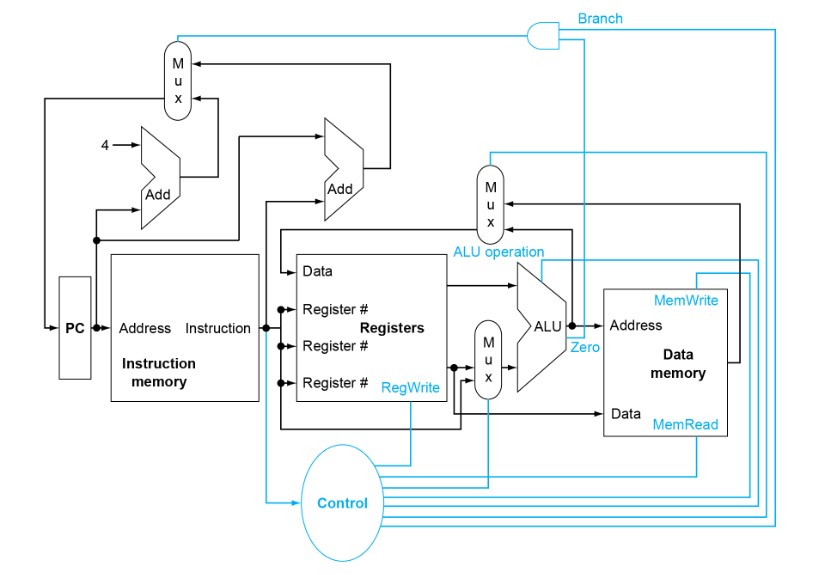
\includegraphics[width = 0.8
        \textwidth]{figures/riscv/risc_2.jpg}
            \caption{\label{risc_2_std} RISC-V Diagram}
        \end{figure}
                    
        
        A processor diagram of the RISC-V CPU can be seen in Figure \ref{risc_2_std}. In the diagram, ``PC'' is the program counter, a 32-bit or 64-bit register; os ``Add'' is an adder; ``Instruction memory'' refers to the component of the processor that stores and supplies the instructions to be executed by the processor; ``Registers'' are small storage units inside the processor that store data and instructions during program execution; ``ALU'' is the arithmetic logic unit; and ``data memory'' is the part of the processor that stores and retrieves data during program execution.
        
        The diagram shows the control unit and its connections in blue. The control unit determines which components should be activated or deactivated, such as the ALU, registers, and multiplexers (MUX), to perform the operations specified by the instructions. The sign in ``RegWrite'' is used to indicate whether the result of an instruction should be rewritten to a register; ``MemRead'' and ``MemWrite'' to indicate whether a memory read or write operation should be performed; ``Branch'' used for implementing conditional branching or jump operations. In control, the ``ALUOperation'' signal can have different values, each corresponding to a specific operation that the ALU should perform. Some common examples of operations controlled by ``ALUOp'' include addition, subtraction, logical operations (AND, OR, XOR), bit shifting, and comparisons. Finally, the ``Zero'' control signal refers to a flag or signal that indicates whether the result of an operation performed by the ALU is equal to zero. This flag is used to make conditional decisions based on the result of a previous operation.
    
    \section{Microcontroller} \label{sec:section_riscv_stud.2}
    
        A microcontroller is a chip that combines a microprocessor with memory, input/output peripherals, and other components needed to perform specific control tasks in an embedded system. It is designed for specific applications that require control, such as embedded systems, industrial automation, consumer electronics devices and more. The microcontroller has integrated resources, such as I/O ports (input/output), analog-digital converters, timers, serial communication and other peripherals that facilitate interaction with the external environment.
        
        In the following section, a microcontroller project using the RISC-V architecture is presented.
        
    
    
    \section{NEORV32 Project} \label{sec:section_riscv_stud.3}
    
        \begin{figure}[!t]
            \begin{center}
                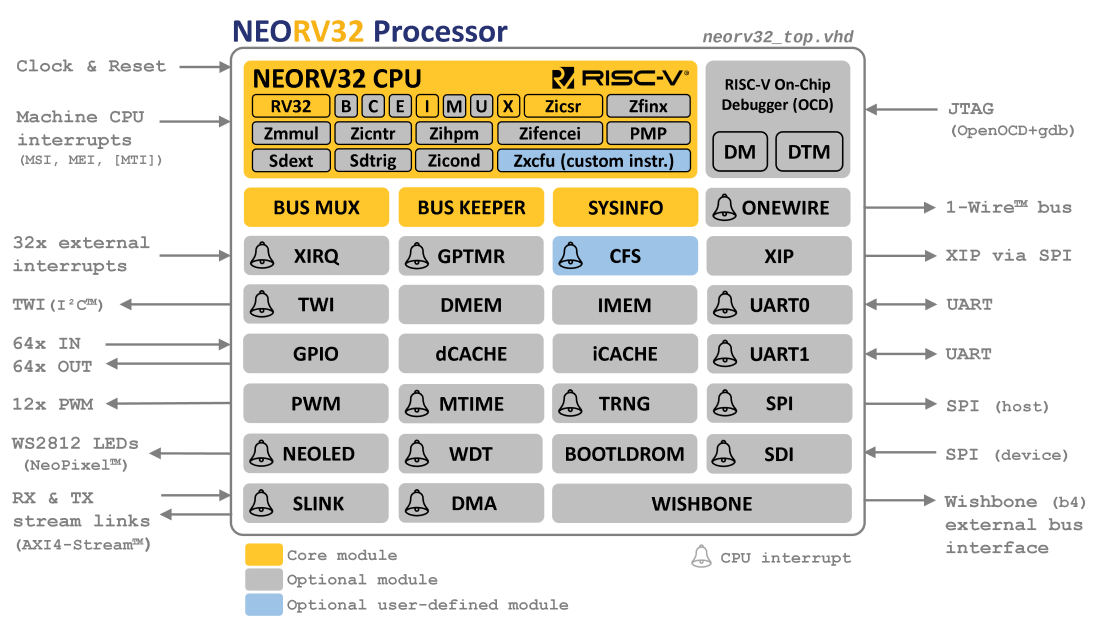
\includegraphics[width=1\textwidth]{figures/neorv32_processor.png}
                \caption{\label{fig:neorv32_peripherals} Representation of the NEORV32 processor, with the available peripherals \cite{nolting_2022}.}
            \end{center}
        \end{figure}
    
        The NEORV32 Project is an open-source, customizable RISC-V processor implementation. It aims to provide a flexible and efficient processor core that can be easily integrated into the FPGA (Field-Programmable Gate Array).
        
        The NEORV32 offers a flexible architecture that allows the connection of multiple peripherals through standard interfaces such as SPI (Serial Peripheral Interface), I2C (Inter-Integrated Circuit), UART (Universal Asynchronous Receiver-Transmitter), GPIO (General Purpose Input/Output). Figure \ref{fig:neorv32_peripherals} shows a diagram of the NEORV32 processor and the components that come with it.
        
        Additionally, the NEORV32 also provides support for external memory, enabling the integration of memory controllers for accessing external storage devices such as flash memory, RAM, SD cards, and others.
        
        The specific peripherals that can be integrated with the NEORV32 depend on the requirements of the project in which it is being used. Some common examples of peripherals that can be added to the NEORV32 include display controllers, audio controllers, network controllers, sensor controllers, wireless communication interfaces, among others. % presents the RISC-V architecture
    \chapter{C Programming for Beginners} \label{chp:chapter_cl}

    Welcome to the \autoref{chp:chapter_cl}, dedicated to the fundamentals of the C language. As an instructor, it is essential to acknowledge that some students may begin their journey in this discipline with limited knowledge of the C language. Understanding this, we have designed this chapter to serve as a gentle reminder and refresher on the crucial concepts that form the building blocks of the C programming.
    
    In the following sections, we will explore key aspects that every student should be familiar with to confidently navigate the world of C programming. These subsections will provide a comprehensive overview of the fundamental components necessary for developing robust and efficient code.
    
    \autoref{sec:section_cl.1}:
    In this subsection, we will delve into the significance of include statements in C programming. Understanding how to use these statements effectively allows us to incorporate external libraries and headers into our code, enabling access to additional functionalities and resources.
    
    \autoref{sec:section_cl.2}:
    Preprocessor definitions play a vital role in C programming as they provide a mechanism for modifying the source code before compilation. In this subsection, we will explore the syntax and usage of preprocessor directives, such as defining constants, macros, and conditional compilation, to enhance the flexibility and versatility of our programs.
    
    \autoref{sec:section_cl.3}:
    Variables are the cornerstone of any programming language, including C. This subsection will revisit the concept of variables, their declaration, and initialization in C. Understanding how to effectively work with variables is essential for storing, manipulating, and retrieving data during program execution.
    
    \autoref{sec:section_cl.4}:
    Operators, conditional statements, and loops form the core control structures in C programming. In this subsection, we will review the different types of operators, explore conditional statements (such as if-else and switch-case), and demonstrate how to use loops (such as for, while, and do-while) to create iterative and decision-making constructs.
    
    \autoref{sec:section_cl.5}:
    Functions provide modularity and code reusability in C programming. In this subsection, we will discuss the importance of functions, their declaration, definition, and usage. Additionally, we will explore function parameters, return types, and the concept of scope, helping students grasp the significance of functions in organizing and structuring their programs effectively.
    
    By immersing ourselves in these sections and reinforcing the fundamental concepts of C programming, both you as the instructor and your students can establish a solid foundation upon which to build further knowledge and expertise in this discipline. So let us embark on this journey and delve into the intricacies of the C language together!
    
    \section{Include Statements} \label{sec:section_cl.1}
        These statements are used to introduce the contents of a separate file into your source file. This is a handy way to keep your code organized, and it also allows you to use library functionality, hardware-configuration routines, and register definitions provided by the manufacturer.
    
            \begin{lstlisting}[style=mystyle_c, language=c, breaklines]
                /************************************************************//**
                 * Includes
                 ***************************************************************/
                #include // SFR declarations
                #include Project_DefsVarsFuncs.h
                #include InitDevice.h
                #include cslib_config.h
                #include cslib.h
            \end{lstlisting}

    \section{Preprocessor Definitions} \label{sec:section_cl.2}

        Preprocessors are programs that process the source code before compilation. A number of steps are involved between writing a program and executing a program in C / C++. Let us have a look at these steps before we actually start learning about Preprocessors.

        \begin{figure}[!ht]
                \centering
                \captionsetup{justification=centering,margin=0.05cm}
                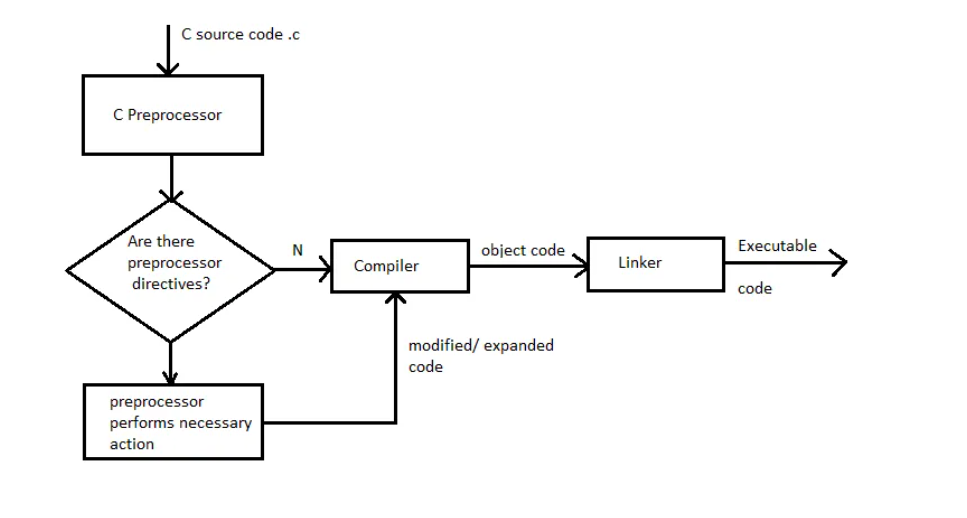
\includegraphics[width=0.8\columnwidth]{figures/preprocessor-in-c.png}
                \caption{\label{fig:preprocessor}Preprocessor in C}
        \end{figure}

        You can see the intermediate steps in the above diagram. The source code written by programmers is first stored in a file, let the name be “program.c“. This file is then processed by preprocessors and an expanded source code file is generated named “program.i”. This expanded file is compiled by the compiler and an object code file is generated named “program.obj”. Finally, the linker links this object code file to the object code of the library functions to generate the executable file “program.exe”. 

        Preprocessor programs provide preprocessor directives that tell the compiler to preprocess the source code before compiling. All of these preprocessor directives begin with a ‘\#’ (hash) symbol. The ‘\#’ symbol indicates that whatever statement starts with a ‘\#’ will go to the preprocessor program to get executed. We can place these preprocessor directives anywhere in our program.

        \begin{figure}[!ht]
                \centering
                \captionsetup{justification=centering,margin=0.05cm}
                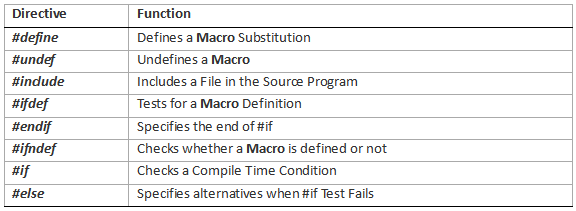
\includegraphics[width=0.8\columnwidth]{figures/preprocessor-directives.png}
                \caption{\label{fig:preprocessor-directives}All the preprocessor directives in C}
        \end{figure}

         Macros are pieces of code in a program that is given some name. Whenever this name is encountered by the compiler, the compiler replaces the name with the actual piece of code. The ‘\#define’ directive is used to define a macro. Syntax of macro definition:

         \begin{lstlisting}[style=mystyle_c, language=c, breaklines]
                #define token value
        \end{lstlisting}
    
    
        For example, let’s say that you’re using the microcontroller’s ADC and that your code uses the ADC’s sample rate in several separate calculations. A preprocessor definition allows you to use an intuitive string (such as SAMPLE\_RATE) instead of the number itself in the calculation code, and if you’re experimenting with different sample rates, you only need to change the one numerical value in the preprocessor definition.
    
            \begin{lstlisting}[style=mystyle_c, language=c, breaklines]
                #define SAMPLE_RATE 100000
            \end{lstlisting}
        
        You can change 100000 to any other number, and this new number will be used to replace all instances of the string SAMPLE\_RATE.

        Preprocessor definitions are also a great way to make code more readable. The following is a list of handy \#define statements.
     
            \begin{lstlisting}[style=mystyle_c, language=c, breaklines]
                #define BIT7 0x80
                #define BIT6 0x40
                #define BIT5 0x20
                #define BIT4 0x10
                #define BIT3 0x08
                #define BIT2 0x04
                #define BIT1 0x02 
                #define BIT0 0x01
                
                #define HIGH 1
                #define LOW 0
                
                #define TRUE 1
                #define FALSE 0
                
                #define SET 1
                #define CLEARED 0
                
                #define LOWBYTE(v)   ((unsigned char) (v))
                #define HIGHBYTE(v)  ((unsigned char) (((unsigned int) (v)) >> 8))
            \end{lstlisting}

        Its important to understand that preprocessor definitions have no direct relationship to hardware. You’re just telling the preprocessor to replace one string of characters with another string of characters before the program is compiled.
    
    \section{Variables} \label{sec:section_cl.3}
        Processors store data in registers and memory locations. There really is no such thing as a variable as far as the hardware is concerned. For the programmer, though, writing code is much easier when we can use intuitively named variables instead of memory addresses or register numbers.
            
        Compilers can manage the low-level details associated with variables without much input from the programmer, but if you want to optimize your use of variables you'll need to know something about the device’s memory configuration and the way in which it handles data of different bit widths.

        \begin{figure}[!ht]
                \centering
                \captionsetup{justification=centering,margin=0.05cm}
                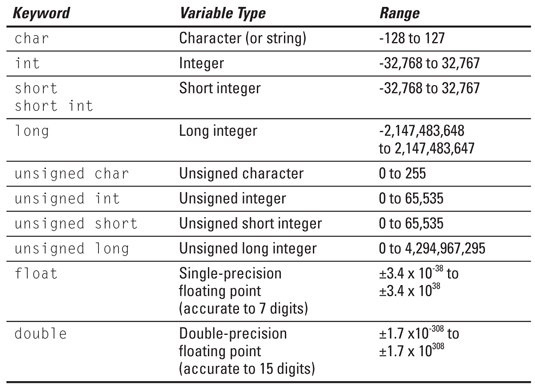
\includegraphics[width=0.8\columnwidth]{figures/variable-in-c.jpg}
                \caption{\label{fig:variable-in-c}Variable types in C}
        \end{figure}
            
        The following code excerpt gives an example of variable definition. This was written for the Keil Cx51 compiler, which reserves one byte of memory for an “unsigned char” definition, two bytes for an “unsigned int” definition, and four bytes for an “unsigned long” definition.
            
                 
            \begin{lstlisting}[style=mystyle_c, language=c, breaklines]
                unsigned long Accumulated_Capacitance_Sensor1;
                unsigned long Accumulated_Capacitance_Sensor2;
                    
                unsigned int Sensor1_Unpressed;
                unsigned int Sensor2_Unpressed;
                    
                unsigned int Sensor1_Measurement;
                unsigned int Sensor2_Measurement;
                    
                unsigned int AngularPosition;
                    
                unsigned int TouchDuration;
                    
                unsigned char CurrentDigit;
                unsigned int CharacterEntry;
                unsigned char DisplayDivider;
            \end{lstlisting}
                

    \section{Operators, Conditional Statements, and Loops} \label{sec:section_cl.4} 
        \subsection{Operators}
        
            The core of computational functionality consists of moving data, performing mathematical computations and logical operations with data, and making programmatic decisions based on the value of stored or generated data.
                
            Mathematical operations and bit manipulation are accomplished by means of operators. C has quite a few operators: equals (=), addition (+), subtraction (-), multiplication (*), division (/), bitwise AND (\&), bitwise OR (|), and so forth. The ``input'' to an operator statement are variables or constants, and the result is stored in a variable. Can you see some operators in \autoref{fig:operators-in-c}.
    
            \begin{figure}[!ht]
                    \centering
                    \captionsetup{justification=centering,margin=0.05cm}
                    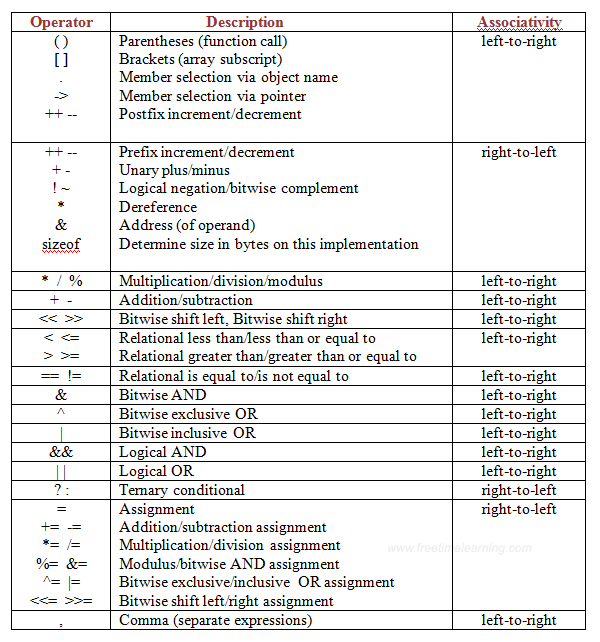
\includegraphics[width=\columnwidth]{figures/operators-in-c.png}
                    \caption{\label{fig:operators-in-c}Operators in C}
            \end{figure}

        \subsection{Conditional Statements}
            
            Conditional statements allow you to perform or not perform an action based on whether a given condition is true or false. These statements use the words \textit{“if”} and \textit{“else”}; for example:
                
                \begin{lstlisting}[style=mystyle_c, language=c, breaklines]
                    if(Sensor1 < Sensor2 && Sensor1 < Sensor3)
                        return SENSOR_1;   
                    else 
                    if(Sensor2 < Sensor1 && Sensor2 < Sensor3)
                        return SENSOR_2;     
                    else 
                    if(Sensor3 < Sensor2 && Sensor3 < Sensor1)
                        return SENSOR_3;     
                    else
                        return 0;
                \end{lstlisting} 
    
            \vspace{2cm}
            
        \subsection{Loop}
            For loops and \textit{while} loops provide a convenient means of repeatedly executing a block of code. These types of tasks arise very frequently in embedded applications. For loops are more oriented toward situations in which a block of code must be executed a specific number of times, and \textit{while} loops are handy when the processor should continue repeating the same block of code until a condition changes from true to false. The \autoref{fig:for-loop} explain the working flow of For loop and \autoref{fig:while-loop} explain the \textit{while} loop.
            
                \begin{figure}[!ht]
                    \centering
                    \captionsetup{justification=centering,margin=0.05cm}
                    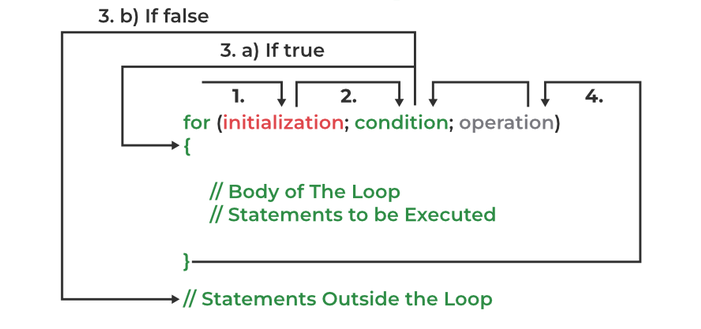
\includegraphics[width=0.8\textwidth]{figures/for-loop.png}
                    \caption{\label{fig:for-loop}For loop in C}
                \end{figure}
    
                \begin{figure}[!ht]
                    \centering
                    \captionsetup{justification=centering,margin=0.05cm}
                    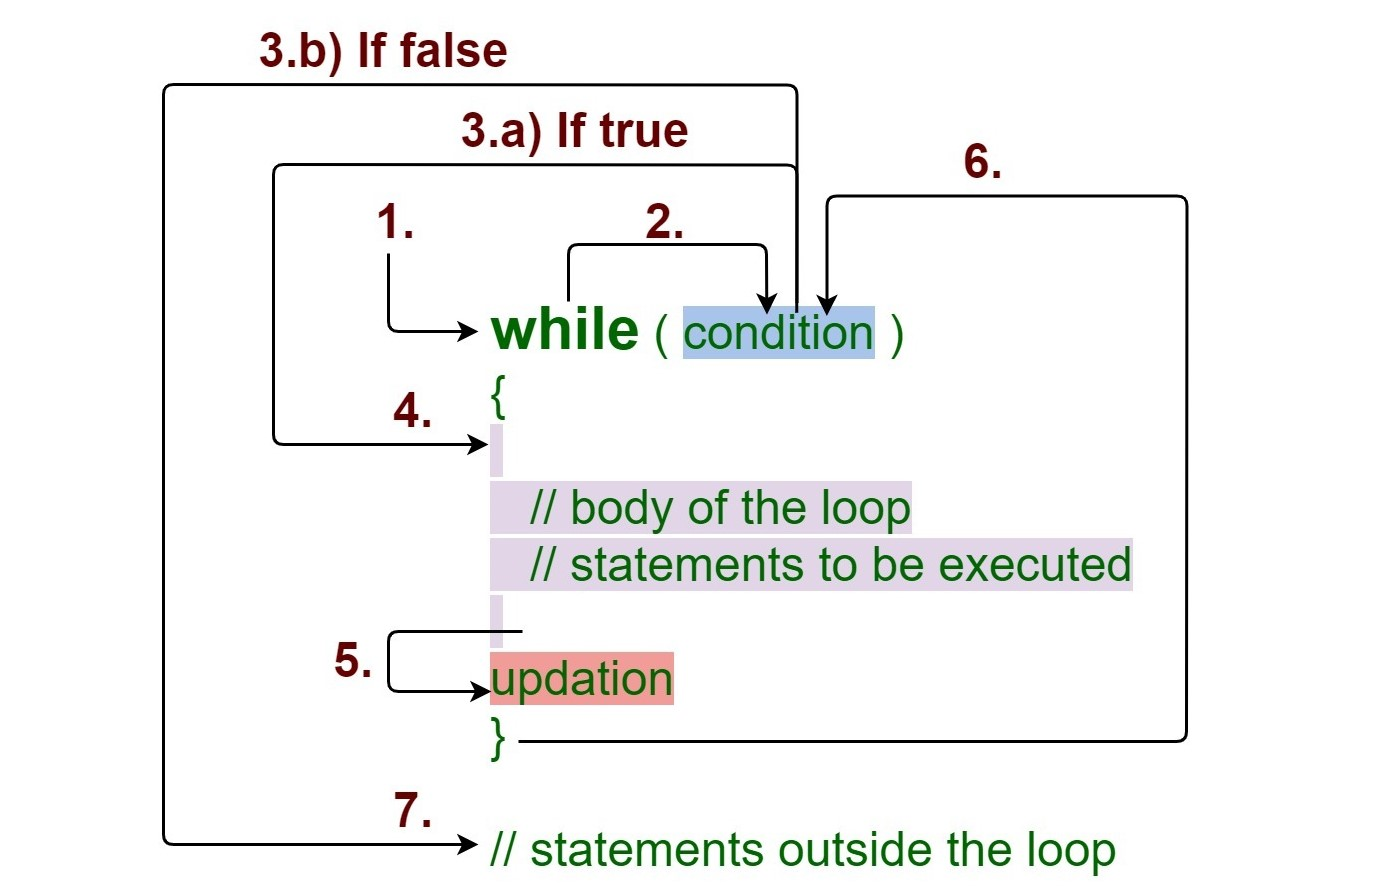
\includegraphics[width=0.7\textwidth]{figures/while-loop.jpg}
                    \caption{\label{fig:while-loop}While loop in C}
                \end{figure}
            \vspace{3cm}
                
            
            Here are examples of both types.
    
                \begin{lstlisting}[style=mystyle_c, language=c, breaklines]
                    for (n = 0; n < 16; n++)
                    {
                        Accumulated_Capacitance_Sensor1 += Measure_Capacitance(SENSOR_1);
                        Delay_us(50);
                        Accumulated_Capacitance_Sensor2 += Measure_Capacitance(SENSOR_2);
                        Delay_us(50);
                    }
                        
                    while(CONVERSION_DONE == FALSE);
                    {
                        LED_STATE = !LED_STATE;
                        Delay_ms(100);
                    }
                    \end{lstlisting}

                    
        \subsection{Switch Case}
            \textit{Switch case} statement evaluates a given expression and based on the evaluated value (matching a certain condition), it executes the statements associated with it. Basically, it is used to perform different actions based on different conditions (cases). 
        
            \begin{itemize}
                \item \textit{Switch case} statements follow a selection-control mechanism and allow a value to change control of execution.
                \item They are a substitute for long if statements that compare a variable to several integral values.
                \item They are a substitute for long if statements that compare a variable to several integral values.
                \item The switch statement is a multiway branch statement. It provides an easy way to dispatch execution to different parts of code based on the value of the expression.
            \end{itemize}
            
            In C, the \textit{switch case} statement is used for executing one condition from multiple conditions. It is similar to an if-else-if ladder.
        
            \begin{figure}[!ht]
                        \centering
                        \captionsetup{justification=centering,margin=0.05cm}
                        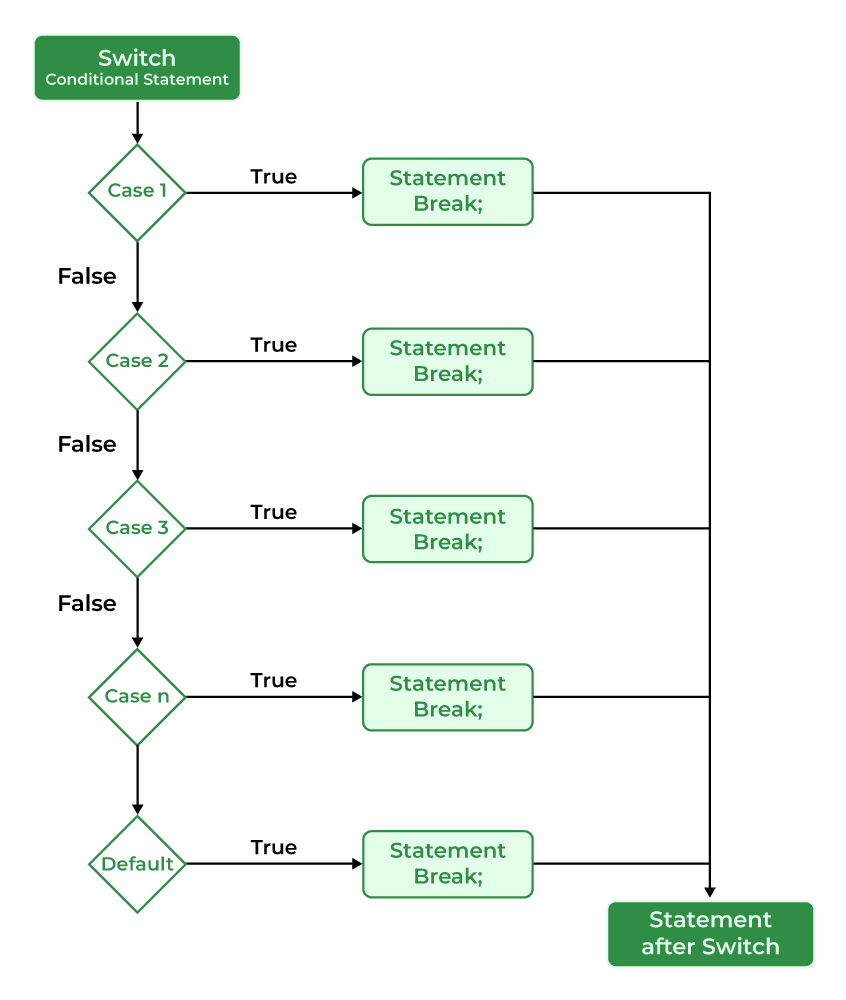
\includegraphics[width=0.7\textwidth]{figures/switch-case-in-c.png}
                        \caption{\label{fig:switch-case-in-c}Switch case in C}
                    \end{figure} 
        
            Here is an example to better understand:
            
            \begin{lstlisting}[style=mystyle_c, language=c, breaklines]
                        // C program to Demonstrate returning of day based numeric
                        // value
                        #include <stdio.h>
                         
                        int main()
                        {
                          // switch variable
                            int var = 1;
                         
                          // switch statement
                            switch (var) {
                                case 1:
                                    printf("Case 1 is Matched.");
                                    break;
                         
                                case 2:
                                    printf("Case 2 is Matched.");
                                    break;
                         
                                case 3:
                                    printf("Case 3 is Matched.");
                                    break;
                         
                                default:
                                    printf("Default case is Matched.");
                                    break;
                            }
                         
                            return 0;
                        }
                        \end{lstlisting}
        
        \subsection{Break and Continue}    
            You have already seen the break statement used in an earlier chapter of this tutorial. Interrupts the execution of a command (switch) or loop (for, while, do-while). The \textit{break} forces the output of the innermost loop.

            The \textit{continues} forces the execution of the next iteration of the loop



    \section{Functions} \label{sec:section_cl.5}

        Good C code is vastly superior to assembly code in terms of organization and readability, and this is due in large part to the use of functions.
            
        Functions are blocks of code that can be easily incorporated into other portions of code. Causing the processor to execute the instructions contained in the function is referred to as “calling” the function. A function can accept one or multiple inputs, and it can provide one output, called a return value.

        In a function declaration \autoref{fig:function-declaration-in-c}, we must provide the function name, its return type, and the number and type of its parameters. A function declaration tells the compiler that there is a function with the given name defined somewhere else in the program.
        The parameter name is not mandatory while declaring functions. We can also declare the function without using the name of the data variables.

        \begin{figure}[!ht]
                \centering
                \captionsetup{justification=centering,margin=0.05cm}
                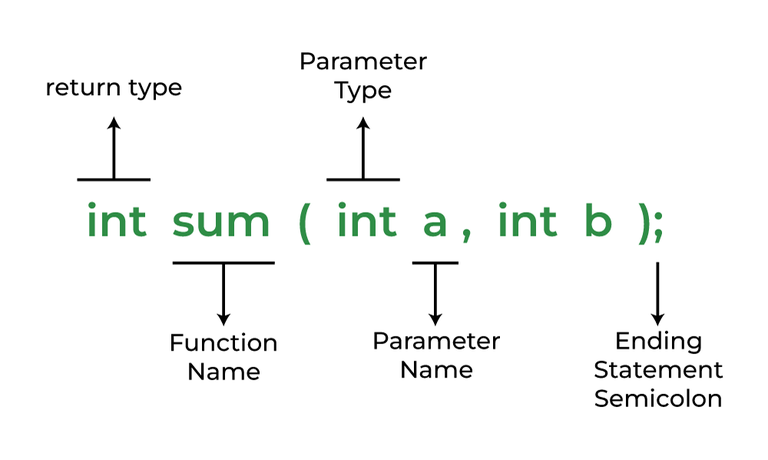
\includegraphics[width=0.7\textwidth]{figures/function-in-c.png}
                \caption{\label{fig:function-declaration-in-c}Function declaration}
        \end{figure}
        \vspace{0.5cm}
        In the below example \autoref{fig:working-of-function-in-c}, the first sum function is called and 10,30 are passed to the sum function. After the function call sum of a and b is returned and control is also returned back to the main function of the program.
        
        \begin{figure}[!ht]
                \centering
                \captionsetup{justification=centering,margin=0.05cm}
                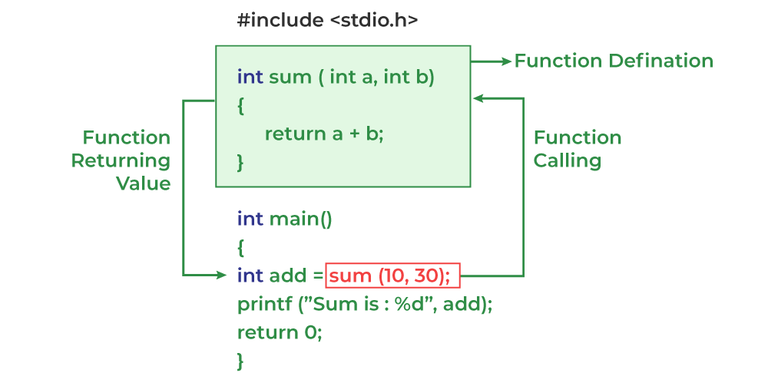
\includegraphics[width=0.7\textwidth]{figures/working-of-function-in-c.png}
                \caption{\label{fig:working-of-function-in-c}Working of Function}
        \end{figure}

        The data passed when the function is being invoked is known as the Actual parameters. In the below \autoref{fig:function-parameters-in-c}, 10 and 30 are known as actual parameters. Formal Parameters are the variable and the data type as mentioned in the function declaration. In the below program, a and b are known as formal parameters.

        \begin{figure}[!ht]
                \centering
                \captionsetup{justification=centering,margin=0.05cm}
                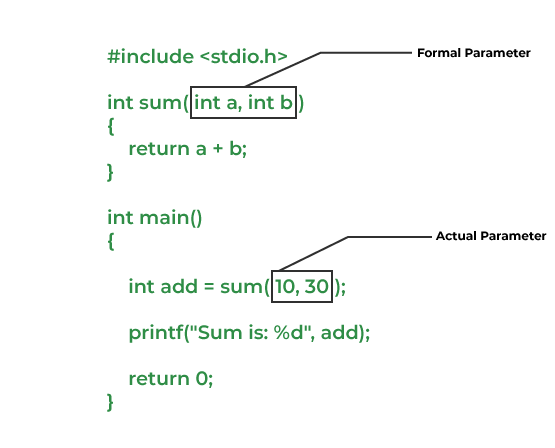
\includegraphics[width=0.7\textwidth]{figures/function-parameters-in-c.png}
                \caption{\label{fig:function-parameters-in-c}Passing parameters to functions}
        \end{figure}
        
        The use of functions does involve some overhead, so we have to be careful to not burden the processor with an excessive number of function calls, but in general the benefits of functions far outweigh the costs.
            
        Here is an example of a function that has three numerical inputs and uses these inputs to generate a true-or-false return value.
            
            \begin{lstlisting}[style=mystyle_c, language=c, breaklines]
                bit Is_In_Range(int input, int LowerBound, int UpperBound)
                {
                    if(input >= LowerBound && input <= UpperBound)
                        return TRUE;
                
                    else
                        return FALSE;
                }
            \end{lstlisting} % presents the c language
    \chapter{NEORV32's space address} \label{chp:chapter_s}

    \begin{figure}[!ht]
        \begin{center}
            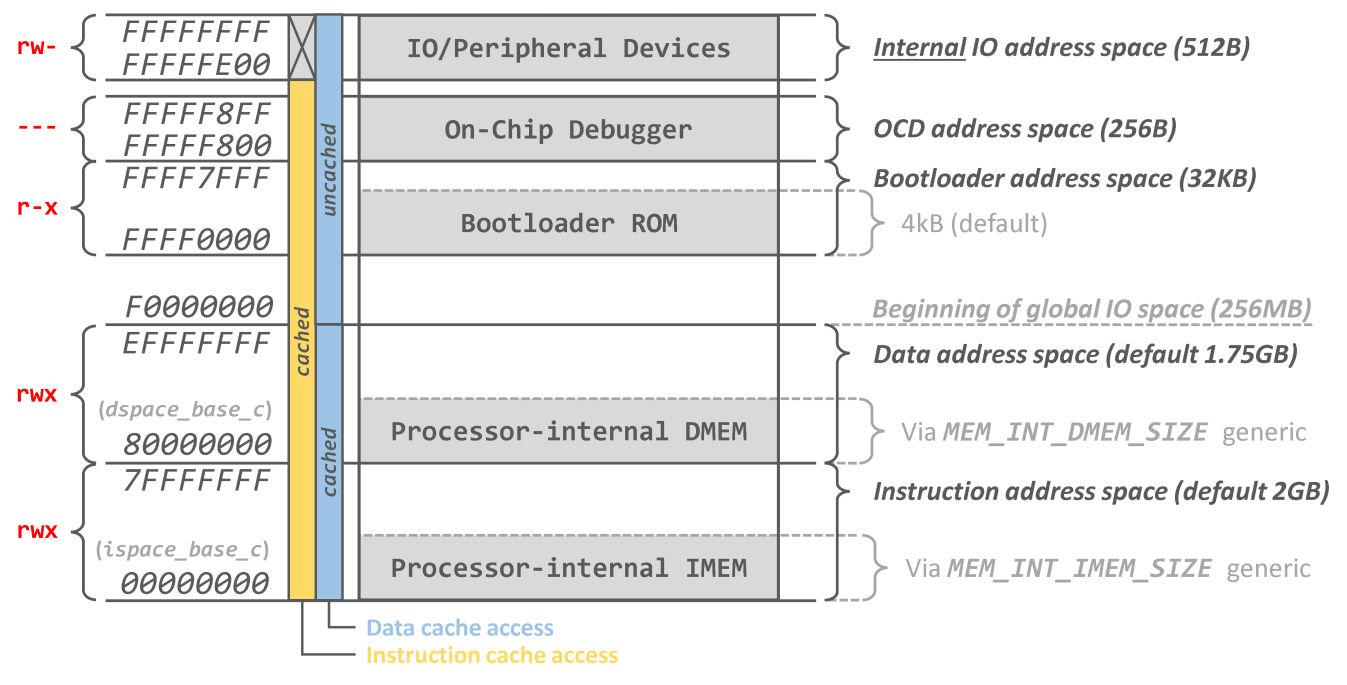
\includegraphics[width=\textwidth]{figures/address_space.png}
            \caption{\label{fig:neorv32_address_space} Representation of the NEORV32's space address.}
        \end{center}
    \end{figure}

    Welcome to the \autoref{chp:chapter_s}. Here we are going to present the NEORV32's memory regions. The NEORV32 is a 32-bit architecture, which have access to up to 4GB memory. By default, this address space is divided into five main regions, as presented in \autoref{fig:neorv32_address_space}.

    \textbf{Instruction address space}: where the code itself and constants are going to be stored. This address space can be referenced as instruction memory (IMEM), and can go from 0x00000000 up to 0x7FFFFFFF.

        \begin{tcolorbox}[colback=blue!5!white,colframe=blue!75!black,title=Extra information]
            The implementation of the processor-internal data memory is enabled via the processor's MEM\_INT\_IMEM\_EN, a generic presented in \textit{neor32\_top.vhd} file. The size in bytes is defined via the MEM\_INT\_IMEM\_SIZE, which is by default 16x1024 bytes.
        \end{tcolorbox}

    \textbf{Data address space}: where the application run-time data (heap, stack, etc.) is stored. This address space can be referenced as data memory (DMEM), and can go from 0x80000000 up to 0xEFFFFFFF.

        \begin{tcolorbox}[colback=blue!5!white,colframe=blue!75!black,title=Extra information]
            The implementation of the processor-internal data memory is enabled via the processor's MEM\_INT\_DMEM\_EN, a generic presented in \textit{neor32\_top.vhd} file. The size in bytes is defined via the MEM\_INT\_DMEM\_SIZE, which is by default 8x1024 bytes.
        \end{tcolorbox}

    \textbf{Bootloader address space}: used for storing an optional built-in firmware that allows to upload new applications into the NEORV32. A UART connection is used to provide a simple text-based user interface that allows to upload the executable. This address space can be referenced as bootloader memory (BOOTROM), and can go from 0xFFFF0000 up to 0xFFFF7FFF.

    \textbf{IO/peripheral address space}: where the processor-internal memory-mapped peripherals are stored. Hence, all peripheral/IO devices are accessed using a memory-mapped scheme. It goes from 0xFFFFFE00 to 0xFFFFFFFF.


\chapter{NEORV32's peripherals}\label{chp:chapter_p}
 
    Welcome to the \autoref{chp:chapter_p}. Here we are going to show the theory behind the main NEORV32's peripherals that should be adapted to be used during the \textit{EEL7030 - Microprocessadores}. As presented in \autoref{fig:neorv32_peripherals}, some of the available peripherals are: UART, SPI, GPIO, PWM, TWI, interrupt controller, embedded memory and timers. Nevertheless, the UART, GPIO, interrupt controller and timers are the implemented ones, as are needed during the \textit{EEL7030}.

    \autoref{sec:section_p.1}: First, we are going to present the GPIO, a peripheral used to interface LEDs, 7-segments displays and LCD of the DE2i-150, as well as switches and buttons. We are going to present this peripheral and its implementation in the development board, showing the defined pin mapping. 
    
    \autoref{sec:section_p.2}: Then, the interrupt controller is presented. It is important to explain the concept of interrupt, trap and exceptions, mechanisms used by CPUs and microprocessor to identify a specific event that requires breaking the on-going execution flow, redirecting it to a interrupt service routine (ISR). The available interrupt sources are going to be presented, showing how to use them in the development board. 
    
    \autoref{sec:section_p.3}: Next, we will introduce timers, which are closely related to the previous peripheral, since they are often used to generate interruptions. Their utilization in the DE2i-150 is presented, too. 
    
    \autoref{sec:section_p.4}: Finally, reaching the end of the covered topics in the \textit{EEL7030}, we have the serial communications. Then, we will present the UART, the serial communication generally used in the course. We are going to explain what is an asynchronous and synchronous communication, how it is handled in the NEORV32 and, finally, show how it was implemented in the development board.
    
    \section{General-purpose input/output (GPIO)}\label{sec:section_p.1}

        The GPIO is composed by a set of programmable input/output pins that are used to provide an interface between external devices and the microprocessor. It can be fairly represented as in \autoref{fig:gpio_representation}. As configured as an output pin, it is possible to set it to high or low level, which means, respectively, VDD (3,3V, 5V or other common value) and GND. In this configuration, we still can read the pin's state. However, when configured as an input pin, it is no longer possible to set the pin's state, only being possible to read its state. The state that the pin should be set to, as well as its current state, is stored in registers, as can be seen in \autoref{fig:gpio_representation}.

        \begin{figure}[!ht]
            \begin{center}
                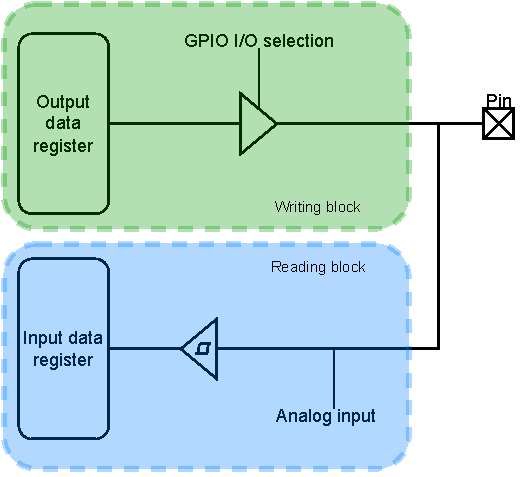
\includegraphics[width= 0.6\textwidth]{figures/gpio_representation.pdf}
                \caption{\label{fig:gpio_representation} Basic representation of a GPIO.}
            \end{center}
        \end{figure}

        \begin{table}[h]

        \centering
            \caption{\label{tab:register_map_gpio} GPIO's memory-mapped registers.}
            \begin{tabular}{ccccc}
                \toprule
                \textbf{Address} & \textbf{Name [C]} & \textbf{Bit(s)} & \textbf{R/W} & \textbf{Function} \\
                \midrule
                \midrule
                0xFFFFFFC0 & INPUT\_LO & 31:0 & r/- & parallel input port pins 31:0 \\ 
                0xFFFFFFC4 & INPUT\_HI & 31:0 & r/- & parallel input port pins 63:32 \\ 
                0xFFFFFFC8 & OUTPUT\_LO & 31:0 & r/w & parallel output port pins 31:0 \\ 
                0xFFFFFFCC & OUTPUT\_HI & 31:0 & r/w & parallel output port pins 63:32 \\ 
                \bottomrule
            \end{tabular}
        \end{table}

        The NEORV32 offers a simple parallel input and output port. These ports can be used chip-externally (for example to drive status LEDs, connect buttons, etc.) or chip-internally.

        \begin{tcolorbox}[colback=blue!5!white,colframe=blue!75!black,title=Extra information]
            The number of input/output pairs that will be available is defined by IO\_GPIO\_NUM, a generic presented in \textit{neor32\_top.vhd} file. When set to zero, the GPIO is excluded from synthesis and the output port is tied to all-zero. If IO\_GPIO\_NUM is less than the 64 (maximum value), only the LSB-aligned bits in gpio\_o and gpio\_i are actually connected while the remaining bits are tied to zero or are left unconnected, respectively.
        \end{tcolorbox}
        
        Furthermore, the GPIO's memory-mapped registers are presented in \autoref{tab:register_map_gpio}. To be able to control the pin's state, you should write to the address named OUTPUT\_HI (GPIO\_o [63:32]) and \textit{OUTPUT\_LO} (GPIO\_o [31:0]). Putting theses bits to ``1'' means that the pins are in high state, then putting them to ``0'' means that they are in low state. And to be able to see pin's states, you could read any of the 4 addresses. 

        Next, it will be presented the adaptation made to make it possible to use the NEORV32's GPIO in the DE2i-150. It will be also presented some theory behind LEDs, 7-segment displays and the LCDs.
        
        \subsection{LEDs}
            As we can see in \autoref{fig:led_fpga_board}, there are 27 user-controllable LEDs on the DE2i-150. Eighteen red LEDs and more 9 green LEDs. Nevertheless, only 8 red LEDs are available in the DE2i-150 (LEDR[8:0]), for general purposes. More 8 green LEDs are also available, to be used as status LEDs. \autoref{tab:ledg_o} and \autoref{tab:ledr_o} shows the assignments of the board's pins to the LEDs. 

            \begin{figure}[!ht]
                \begin{center}
                    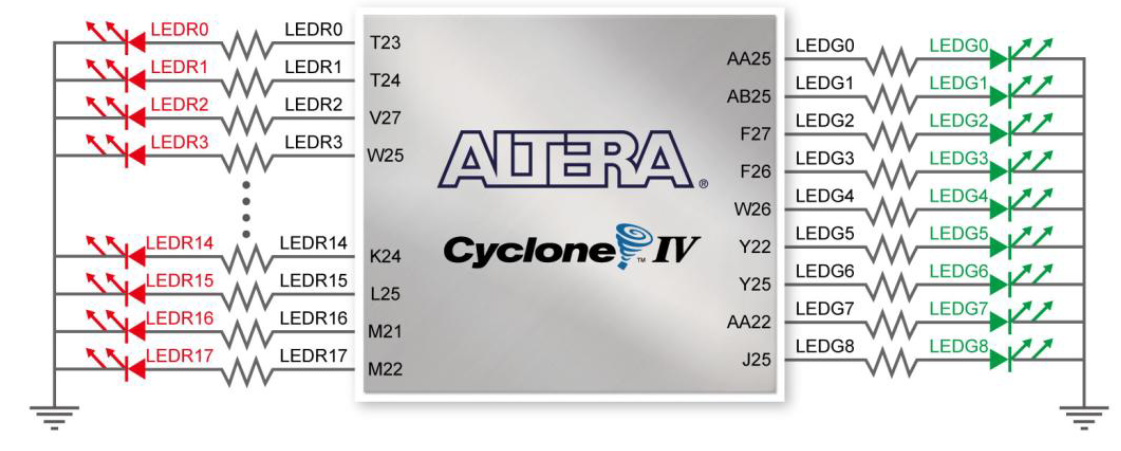
\includegraphics[width= 0.6\textwidth]{figures/led_fpga_board.png}
                    \caption{\label{fig:led_fpga_board} Available LEDs on the development board.}
                \end{center}
            \end{figure}
            
        \subsection{7-segment display}
           A 7-segment display is nothing more than a set of LEDs, positioned in such a way that they can form numbers and characters when correctly driven. The DE2i-150 has eight of these displays. Each segment is identified by an index, from 0 to 6, as presented in \autoref{figure:hex}. It is important to point out that each of these segments is going to be set to a high state when the pins connected to them are in low state. The \autoref{tab:hex} shows the assignments of the board's pins to the 7-segment displays.
            
                \begin{figure}[!ht]
                    \begin{center}
                        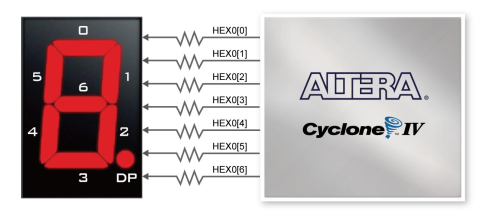
\includegraphics[width= 0.6\textwidth]{figures/chap2/hex.png}
                        \caption{\label{figure:hex} Connections between the 7-segment display HEX0 and Cyclone IV GX FPGA}
                    \end{center}
                \end{figure}
        
        \subsection{LCD}
            The DE2i-150 has a built-in LCD (the HD44780), too, and can be used to display text by sending appropriate commands to the display's controller. As presented in \autoref{figure:lcd}, there are some important signals to properly command de LCD: ON, DATA[7:0], EN, RS an RW. Basically, the LCD\_ON is used to power the LCD. The LCD\_DATA0 to LCD\_DATA7 are used to send a specific command (for instance, 38h, which is the command to define the interface and how many lines are going to be used) or to send a character in the display. Furthermore, LCD\_RW is used to define if we are going to read or write to the display and LCD\_RS is used to distinguish a read/write command from a read/write data to the LCD. Finally, the LCD\_EN is used to actually send the command and/or data whenever it is pulsed. The \autoref{tab:lcd_o} and \autoref{figure:lcd} shows the assignments of the board's pins to the LCD.
                
            \begin{figure}[!ht]
                \begin{center}
                    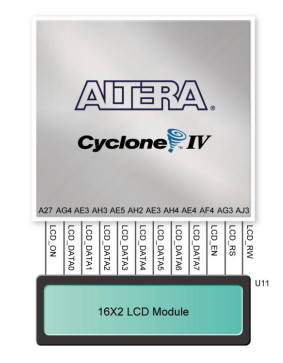
\includegraphics[width= 0.4\textwidth]{figures/chap2/lcd.png}
                    \caption{\label{figure:lcd} Connections between the LCD and Cyclone IV GX FPGA}
                \end{center}
            \end{figure}

        \subsection{Input/output pins}
            The DE2i-150 has 36 pins that can be used as input/output pins, as presented in \autoref{fig:pins_fpga_board}. But only 16 pins are going to be available to be used, where half are used as output pins and the other half as input pins. The \autoref{tab:gpio_o} and \autoref{tab:gpio_i} shows the assignments of the board's pins.
        
            \begin{figure}[!ht]
                \begin{center}
                    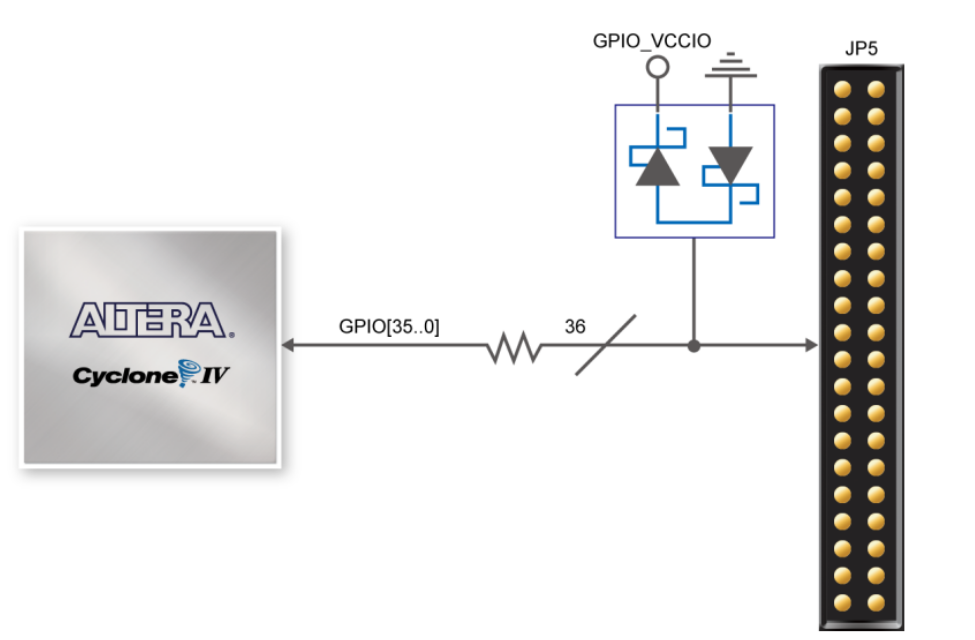
\includegraphics[width= 0.6\textwidth]{figures/pins_fpga_board.png}
                    \caption{\label{fig:pins_fpga_board} Available switches on the development board.}
                \end{center}
            \end{figure}    
        
        \subsection{Switches}
            The DE2i-150 offers 18 switches that can be used during a specific application. But only 8 are going to be available, which are connected to the NEORV32's input pins. The \autoref{tab:sw_i} shows the assignments of the board's switches.
            
            \begin{figure}[!ht]
                \begin{center}
                    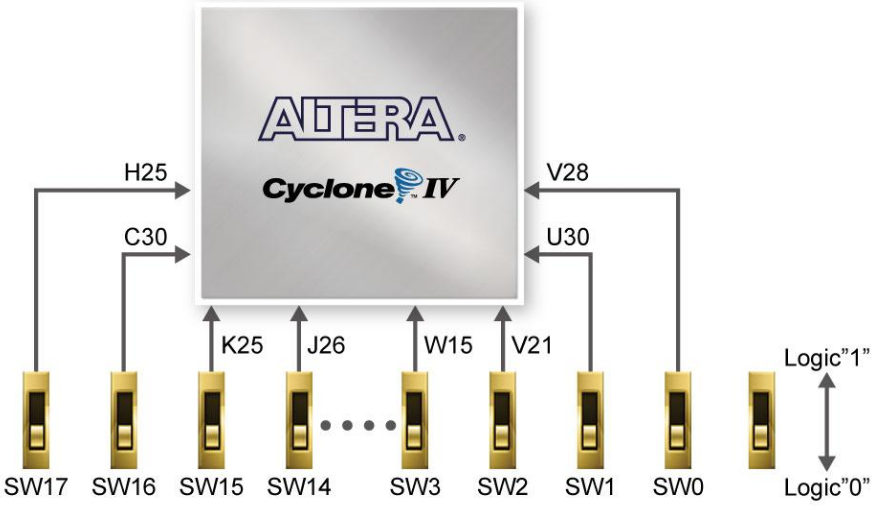
\includegraphics[width= 0.6\textwidth]{figures/sw_fpga_board.png}
                    \caption{\label{fig:sw_fpga_board} Available switches on the development board.}
                \end{center}
            \end{figure}
        
    \section{Interrupt controller}\label{sec:section_p.2}

        To present this peripheral, it is important to define some concepts, such as interruptions, exceptions and traps in a RISC-V architecture. Then, the way in which the microprocessor identifies the interrupt's source, its priority, and the way to handle it needs to be presented, too.
    
        \subsection{Interruptions, exceptions and traps}
    
            First, it is necessary to define interruptions, exceptions and traps. In a RISC-V architecture, interruptions and exceptions will generate a disruption of the on-going execution flow, so that the microprocessor can properly handle a specific event. However, this can occur in two ways: synchronously or asynchronously.
        
            Based on the definitions used in the RISC-V documentation \cite{panesar_2022}, an exception is a synchronous event, as it is a response to some exceptional and unusual condition due to program execution. For instance, some conditions that may raise (cause) an exception include executing a division instruction with a zero divisor, executing an illegal opcode, and a memory protection fault. 
    
    	    Interruption, on the other hand, is an asynchronous event, as it is generated by an external hardware event (which would be external to the microprocessor). These interrupts generally have nothing at all to do with the instructions currently executing; instead, some event, such as pressing a button or a timeout on a timer, informs the microprocessor that a device needs some attention.
    
            Last but not least, in this context, a trap is the transfer of control to a trap handler to determine whether the incoming trap is an interrupt or an exception and call an appropriate handler.
    
    	    When these events occur, the PC register must be saved somewhere, so the microprocessor can resume. Then after handling the event it is possible to load the PC register to continue with the previous execution flow.

        \subsection{Interrupts and exceptions handling}

            To adequately handling the interruptions and exceptions, the NEORV32 has a specific control and status registers (CSRs) for that, which is presented in \autoref{tab:interrupt_csr}. It is composed by 5 CSRs. The most significant bit of mcause will store the interruption's cause (is set to ``1'' if it was generated by an interrupt and ``0'' for an exception). The mip has information regarding the pending interrupts and exceptions waiting to be handled. As presented in \autoref{tab:exception_definitions} and \autoref{tab:interrupt_definitions}\footnotemark, each interrupt and exception have its own priority, so if more than one interrupt happens at the same time, the one with the highest one will be handled first. 

            \footnotetext{\textbf{I-PC}: address of interrupted instruction (instruction has not been executed yet); \textbf{PC}: address of instruction that caused the trap (instruction has been executed); \textbf{ADR}: bad memory access address that caused the trap; \textbf{CMD}: the instruction word that caused the trap (zero-extended if compressed instruction); \textbf{0}: zero.}            

            \begin{table}[!ht]
                \centering
                \caption{Machine trap handling CSRs.}
                \adjustbox{max width=\textwidth}{
                    \begin{tabular}{ccccc}
                        \toprule
                        \textbf{Address} & \textbf{Name [ASM]} & \textbf{Name [C]} & \textbf{ACC} & \textbf{Function} \\
                        \midrule
                        \midrule
                        0x340 & mscratch & CSR\_MSCRATCH & MRW & Machine scratch register \\
                        0x341 & mepc & CSR\_MEPC & MRW & Machine exception program counter \\ 
                        0x342 & mcause & CSR\_MCAUSE & MRW & Machine trap cause \\ 
                        0x343 & mtval & CSR\_MTVAL & MRW & Machine bad address or instruction \\ 
                        0x344 & mip & CSR\_MIP & MRW & Machine interrupt pending register \\ 
                        \bottomrule
                    \end{tabular}
                }
                \label{tab:interrupt_csr}
            \end{table}

            \begin{table}[H]
                \centering
                \caption{Exceptions (synchronous to instruction execution).}
                \adjustbox{max width=\textwidth}{
                    \begin{tabular}{cccccc @{}}
                        \toprule
                        \textbf{Prio.} & \textbf{mcause} & \textbf{ID [C]} & \textbf{Cause} & \textbf{mepc} & \textbf{mtval} \\ 
                        \midrule
                        \midrule
                        1 & 0x00000000 & TRAP\_CODE\_I\_MISALIGNED & instruction address misaligned & I-PC & 0 \\ 
                        2 & 0x00000001 & TRAP\_CODE\_I\_ACCESS & instruction access bus fault & I-PC & 0 \\ 
                        3 & 0x00000002 & TRAP\_CODE\_I\_ILLEGAL & illegal instruction & PC & CMD \\ 
                        4 & 0x0000000B & TRAP\_CODE\_MENV\_CALL & environment call from M-mode & PC & 0 \\ 
                        5 & 0x00000008 & TRAP\_CODE\_UENV\_CALL & environment call from U-mode & PC & 0 \\ 
                        6 & 0x00000003 & TRAP\_CODE\_BREAKPOINT & software breakpoint / trigger firing & PC & PC \\ 
                        7 & 0x00000006 & TRAP\_CODE\_S\_MISALIGNED & store address misaligned & PC & ADR \\ 
                        8 & 0x00000004 & TRAP\_CODE\_L\_MISALIGNED & load address misaligned & PC & ADR \\ 
                        9 & 0x00000007 & TRAP\_CODE\_S\_ACCESS & store access bus fault & PC & ADR \\ 
                        10 & 0x00000005 & TRAP\_CODE\_L\_ACCESS & load access bus fault & PC & ADR \\ 
                        \bottomrule
                    \end{tabular}
                }
            \label{tab:exception_definitions}
        \end{table}

        \begin{table}[H]
            \centering
            \caption{Interrupts (asynchronous to instruction execution).}
            \adjustbox{max width=\textwidth}{
                \begin{tabular}{@{} cccccc}
                    \toprule
                    \textbf{Prio.} & \textbf{mcause} & \textbf{ID [C]} & \textbf{Cause} & \textbf{mepc} & \textbf{mtval} \\ 
                    \midrule
                    \midrule
                    11 & 0x80000010 & TRAP\_CODE\_FIRQ\_0 & fast interrupt request channel 0 & I-PC & 0 \\ 
                    12 & 0x80000011 & TRAP\_CODE\_FIRQ\_1 & fast interrupt request channel 1 & I-PC & 0 \\ 
                    13 & 0x80000012 & TRAP\_CODE\_FIRQ\_2 & fast interrupt request channel 2 & I-PC & 0 \\ 
                    14 & 0x80000013 & TRAP\_CODE\_FIRQ\_3 & fast interrupt request channel 3 & I-PC & 0 \\ 
                    15 & 0x80000014 & TRAP\_CODE\_FIRQ\_4 & fast interrupt request channel 4 & I-PC & 0 \\ 
                    16 & 0x80000015 & TRAP\_CODE\_FIRQ\_5 & fast interrupt request channel 5 & I-PC & 0 \\ 
                    17 & 0x80000016 & TRAP\_CODE\_FIRQ\_6 & fast interrupt request channel 6 & I-PC & 0 \\ 
                    18 & 0x80000017 & TRAP\_CODE\_FIRQ\_7 & fast interrupt request channel 7 & I-PC & 0 \\ 
                    19 & 0x80000018 & TRAP\_CODE\_FIRQ\_8 & fast interrupt request channel 8 & I-PC & 0 \\ 
                    20 & 0x80000019 & TRAP\_CODE\_FIRQ\_9 & fast interrupt request channel 9 & I-PC & 0 \\ 
                    21 & 0x8000001a & TRAP\_CODE\_FIRQ\_10 & fast interrupt request channel 10 & I-PC & 0 \\ 
                    22 & 0x8000001b & TRAP\_CODE\_FIRQ\_11 & fast interrupt request channel 11 & I-PC & 0 \\ 
                    23 & 0x8000001c & TRAP\_CODE\_FIRQ\_12 & fast interrupt request channel 12 & I-PC & 0 \\ 
                    24 & 0x8000001d & TRAP\_CODE\_FIRQ\_13 & fast interrupt request channel 13 & I-PC & 0 \\ 
                    25 & 0x8000001e & TRAP\_CODE\_FIRQ\_14 & fast interrupt request channel 14 & I-PC & 0 \\ 
                    26 & 0x8000001f & TRAP\_CODE\_FIRQ\_15 & fast interrupt request channel 15 & I-PC & 0 \\ 
                    27 & 0x8000000B & TRAP\_CODE\_MEI & machine external interrupt (MEI) & I-PC & 0 \\ 
                    28 & 0x80000003 & TRAP\_CODE\_MSI & machine software interrupt (MSI) & I-PC & 0 \\ 
                    29 & 0x80000007 & TRAP\_CODE\_MTI & machine timer interrupt (MTI) & I-PC & 0 \\ 
                    \bottomrule
                \end{tabular}
            }
            \label{tab:interrupt_definitions}
        \end{table}

            \begin{tcolorbox}[colback=blue!5!white,colframe=blue!75!black,title=Extra information]
                The XIRQ provides up to 32 external interrupt channels configured via the XIRQ\_NUM\_CH, a generic presented in \textit{neor32\_top.vhd} file. Each bit in the xirq\_i input signal vector represents one interrupt channel. If less than 32 channels are configured, only the LSB-aligned channels are used while the remaining ones are left unconnected internally. The actual interrupt trigger type is configured before synthesis using the XIRQ\_TRIGGER\_TYPE and XIRQ\_TRIGGER\_POLARITY, two generics presented in the \textit{neor32\_top.vhd}.
            \end{tcolorbox}
    
            The fast interrupt requests (FIRQs) are better presented in \autoref{fig:firqs}. It is possible to understand what kind of interruptions are available in the NEORV32, furthermore, their priority. It is possible to visualize that the external interrupts has their ``sub-priorities'', which are defined by the external interrupt controller (XIRQ). Its memory map is presented in \autoref{tab:firqs}. It works simmilarly to the ``main interrupt controller'', but specifically for the external ones. 

            \begin{figure}[!ht]
                \begin{center}
                    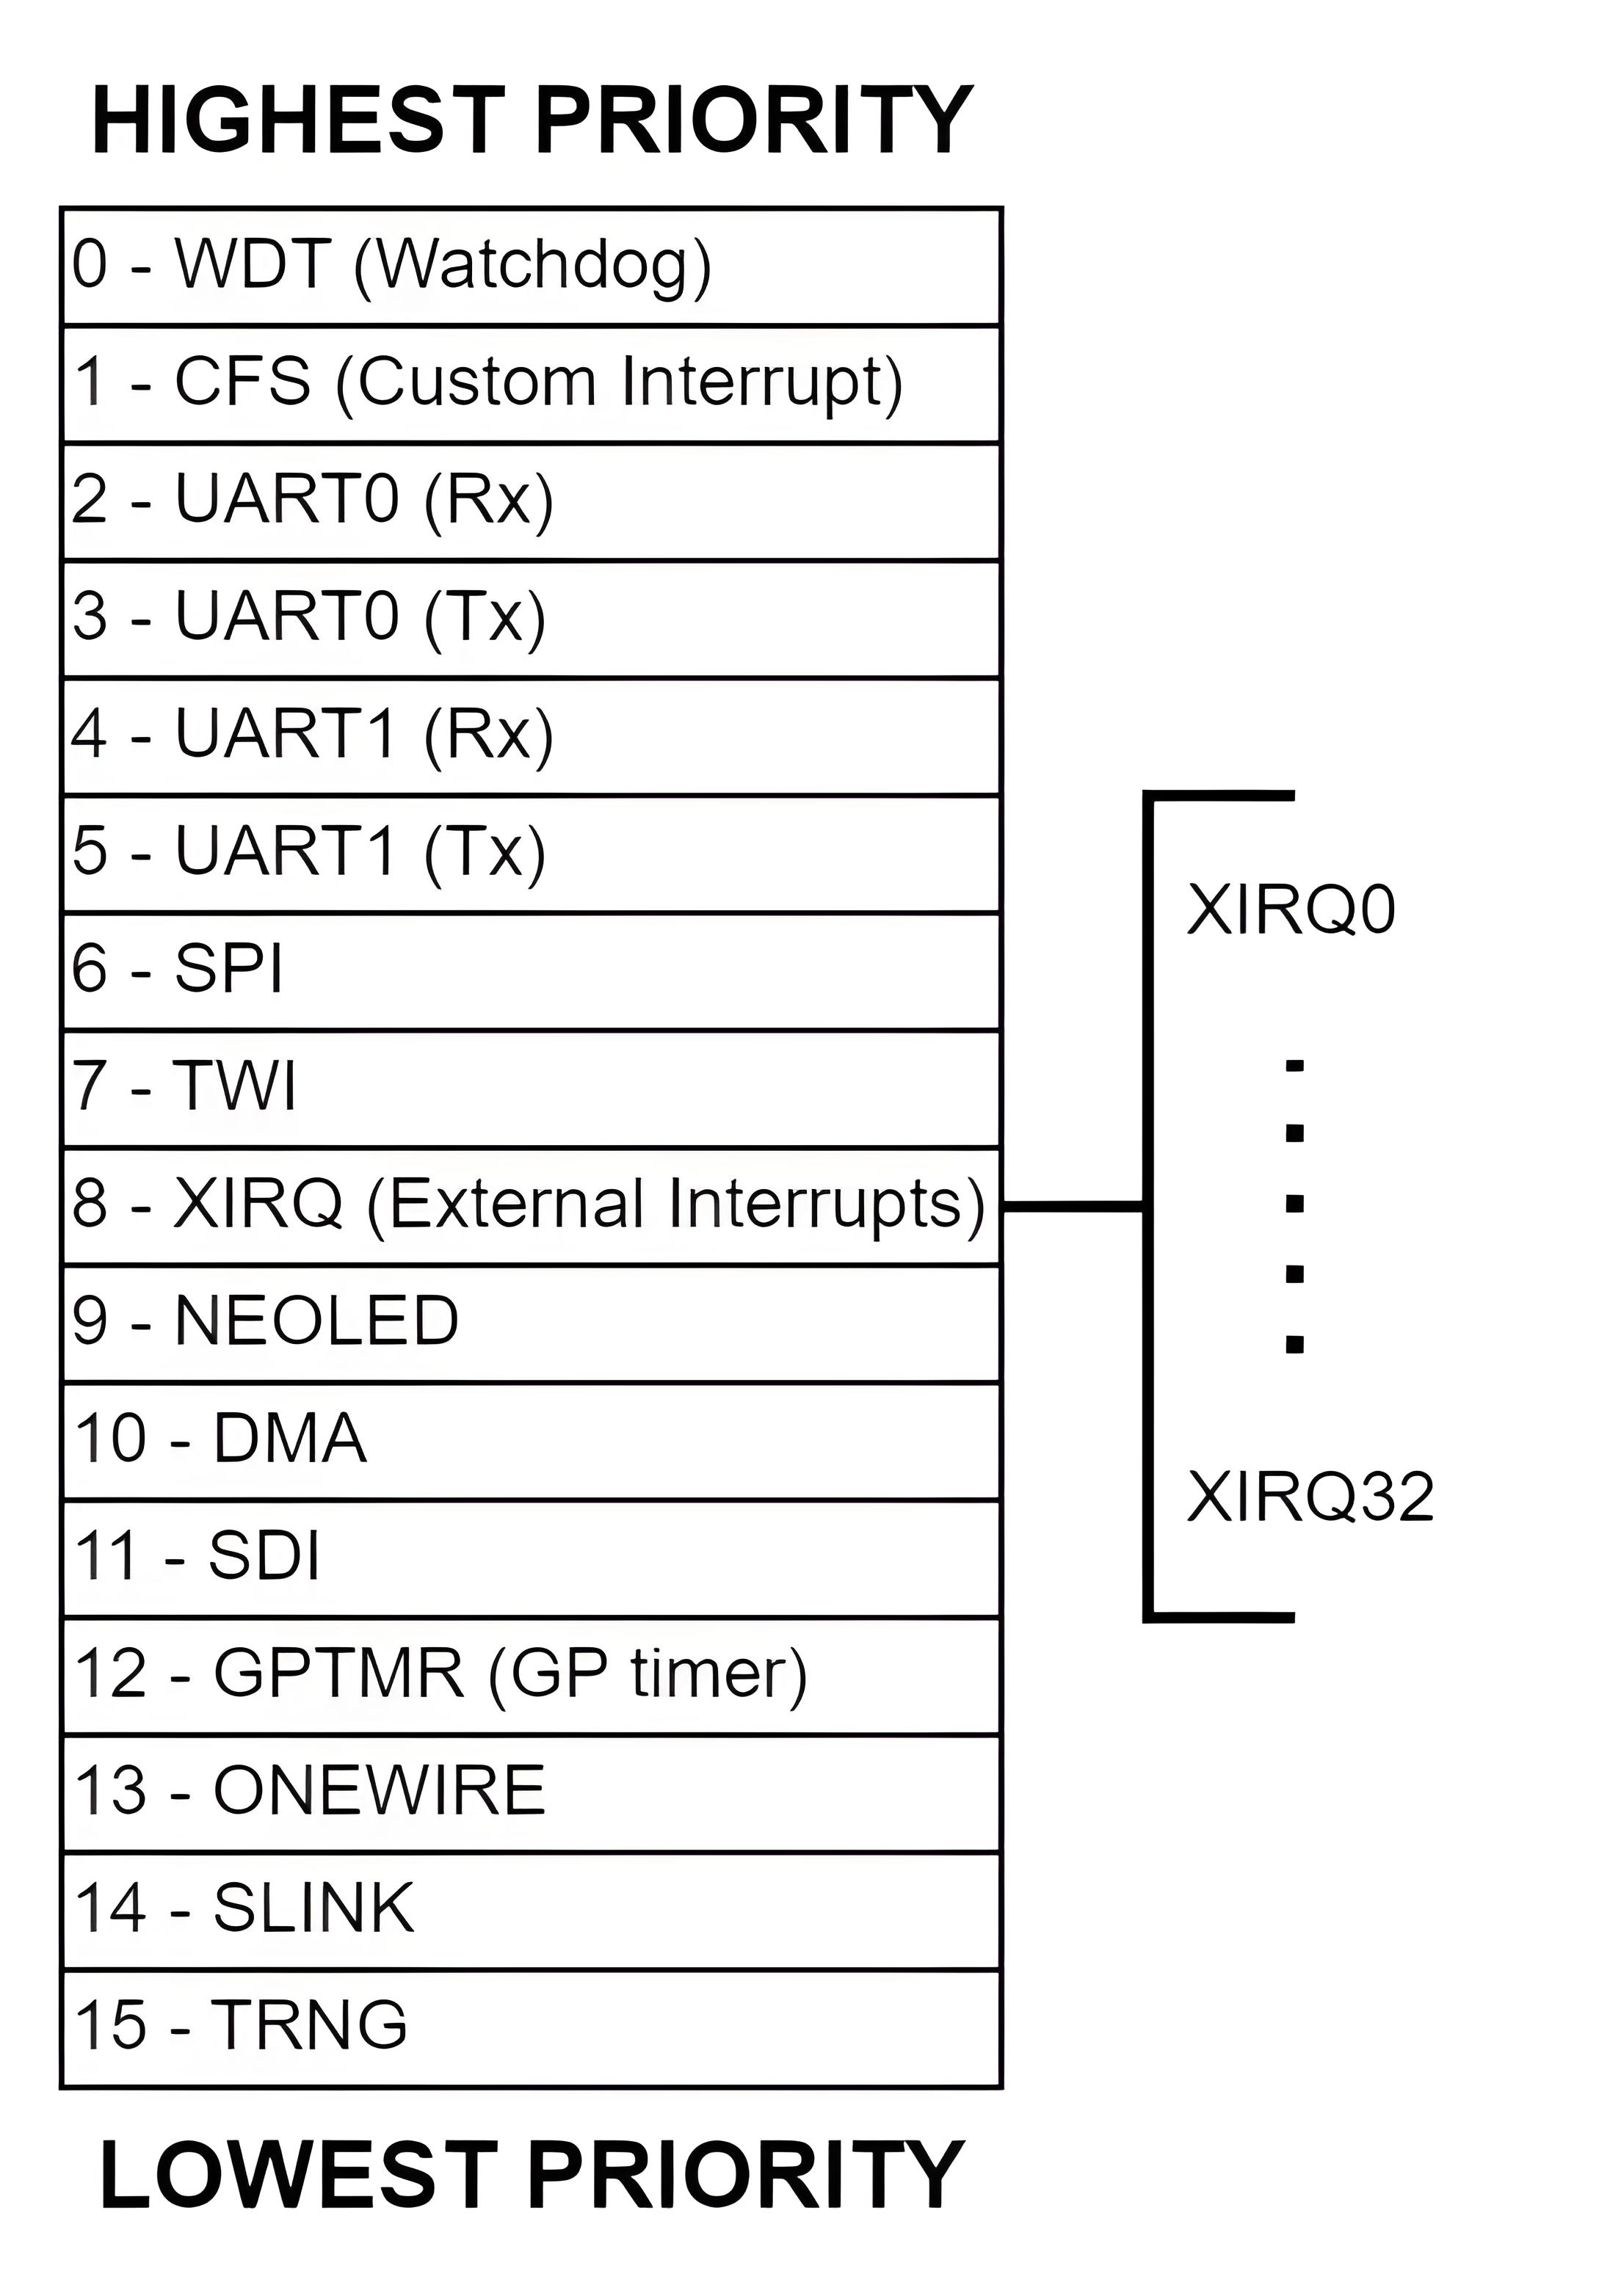
\includegraphics[width= 0.4\textwidth]{figures/firqs.jpeg}
                    \caption{Fast interrupt requests (FIRQs) available.}
                    \label{fig:firqs}
                \end{center}
            \end{figure}

            \begin{table}[!ht]
                \centering
                \caption{XIRQ's memory-mapped registers.}
                \adjustbox{max width=\textwidth}{
                    \begin{tabular}{ccccp{6cm}}
                        \toprule
                        \textbf{Address} & \textbf{Name [C]} & \textbf{Bit(s)} & \textbf{R/W} & \textbf{Description} \\
                        \midrule
                        \midrule
                        0xFFFFFF80 & EIE & 31:0 & r/w & External interrupt enable register (one bit per channel, LSB-aligned) \\
                        0xFFFFFF84 & EIP & 31:0 & r/w & External interrupt pending register (one bit per channel, LSB-aligned); writing 0 to a bit clears the according pending interrupt \\
                        0xFFFFFF88 & ESC & 4:0 & r/w & Interrupt source ID (0..31) of firing IRQ (prioritized!); writing any value will acknowledge the current XIRQ interrupt \\
                        0xFFFFFF8C & - & 31:0 & r/- & Reserved, read as zero \\
                        \bottomrule
                    \end{tabular}
                }
                \label{tab:firqs}
            \end{table}

        \subsection{Input pins and push-buttons}
            The DE2i-150 many ways to interface external devices to generate interruptions. For instance, it has 18 switches that can be used during a specific application, as presented in \autoref{fig:bt_fpga_board}. Only 8 are going to be available, which are connected to the NEORV32's input pins. 

            Furthermore, as presented earlier in \autoref{fig:pins_fpga_board}, it also offer many pins that can be used, too. Here, only two of them are going to be used for generating interruptions.
            
            The \autoref{tab:xirq_i} shows the assignments of the board's switches and pins to be used as interrupt generators.
            
            \begin{figure}[!ht]
                \begin{center}
                    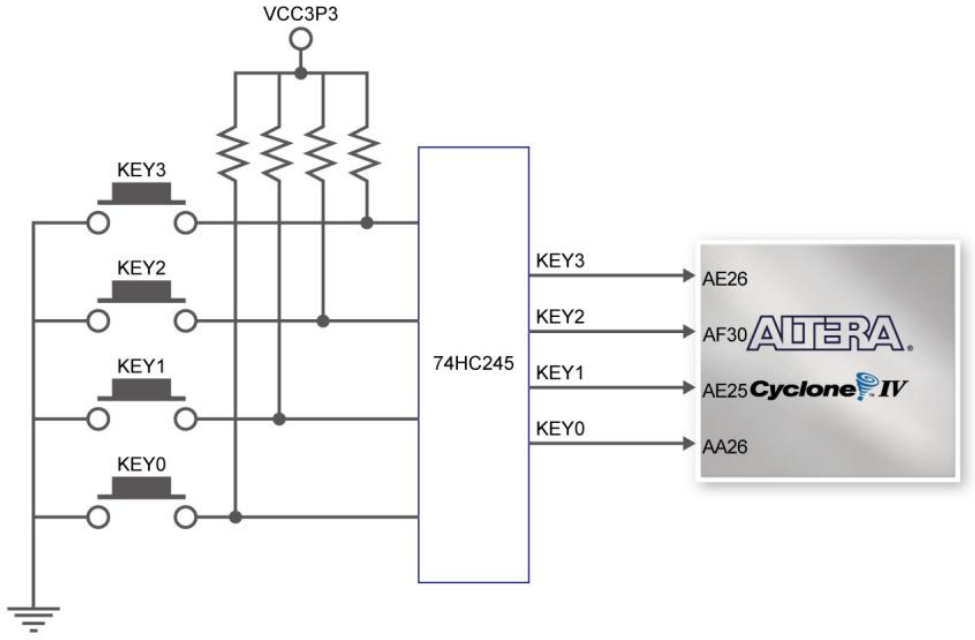
\includegraphics[width= 0.6\textwidth]{figures/bt_fpga_board.png}
                    \caption{\label{fig:bt_fpga_board} Available buttons on the development board.}
                \end{center}
            \end{figure}

    \section{Timers}\label{sec:section_p.3}

        In a microprocessor we can use timers to track time-based events. A timer can be defined as a specialized clock used to measure time intervals. It can function as a stopwatch, counting up from zero or counting down from a set instant. They are often used to generate delays or track the elapsed time. 

        \begin{table}[!ht]
        	\centering
        	\caption{MTIME's memory-mapped registers.}
        	\begin{tabular}{ccccp{4cm}}
        		\toprule
        		\textbf{Address} & \textbf{Name [C]} & \textbf{Bits} & \textbf{R/W} & \textbf{Function} \\
        		\midrule
        		\midrule
        		0xFFFFFF90 & TIME\_LO & 31:0 & r/w & Machine system time, low word \\
        		0xFFFFFF94 & TIME\_HI & 31:0 & r/w & Machine system time, high word \\
        		0xFFFFFF98 & TIMECMP\_LO & 31:0 & r/w & Time compare, low word \\
        		0xFFFFFF9C & TIMECMP\_HI & 31:0 & r/w & Time compare, high word \\
        		\bottomrule
        	\end{tabular}
        	\label{tab:register_map_mtime}
        \end{table}

        In the NEORV32 we have access to the machine system timer (MTIME), which implements a memory-mapped machine timer. It is possible to access the 64-bit system's time via the memory-mapped TIME\_LO and TIME\_HI registers. To configure the timer's interruption, it is necessary to write to other 64-bit registers, which are accessible via the memory-mapped TIMECMP\_LO and TIMECMP\_HI. The interrupt is triggered whenever the content of TIME\_LO and TIME\_HI is greater than or equal to the content of TIMECMP\_LO and TIMECMP\_HI. The interrupt remains active (pending) until TIME\_* becomes less TIMECMP\_* again (either by modifying TIME\_* or TIMECMP\_*). These memories are presented in \autoref{tab:register_map_mtime}, which presents the MTIME's memory map.

        The NEORV32 offers a 32-bit timer, too, the general purpose timer (GPTMR). Its operation is fairly similar to the MTIME. In this peripheral, a 32-bit counter is incremented, which are memory-mapped to COUNT, until reaches the same value stored in the threshold register, the THRES. 

        But in this case it is possible to configure its clock prescaler and its operation mode. For instance, writing to the register GPTMR\_CTRL\_PRSC[2:0], the clock prescaler is configured as presented in \autoref{tab:clock_prescaler}.

        \begin{table}[!ht]
        	\centering
        	\caption{Configuring the clock prescaler}
        	\begin{tabular}{cc}
        		\toprule
        		\textbf{GPTMR\_CTRL\_PRSCx} & \textbf{Resulting clock prescaler} \\
        		\midrule
        		0b000 & 2 \\
        		0b001 & 4 \\
        		0b010 & 8 \\
        		0b011 & 64 \\
        		0b100 & 128 \\
        		0b101 & 1024 \\
        		0b110 & 2048 \\
        		0b111 & 4096 \\
        		\bottomrule
        	\end{tabular}
        	\label{tab:clock_prescaler}
        \end{table}

        Furthermore, it is possible to configure it tu operate in two modes. It is configured trough the GPTMR\_CTRL\_MODE register. If GPTMR\_CTRL\_MODE is equal to ``0'' the timer operates in single-shot mode. So, as soon as COUNT matches THRES an interrupt request is generated and the timer stops its operation (it stops incrementing). However, if GPTMR\_CTRL\_MODE is equal to ``1'' the timer operates in continuous mode. When COUNT matches THRES an interrupt request is generated, but COUNT is automatically reset to all-zero, and then start to increment again. These memories are presented in \autoref{tab:register_map_gptmr}, which presents the GPTMR's memory map.

        \begin{table}[!ht]
        	\centering
        	\caption{GPTMR's memory-mapped registers.}
        	\adjustbox{max width=\textwidth}{
        		\begin{tabular}{ccccp{5cm}}
        			\toprule
        			\textbf{Address} & \textbf{Name [C]} & \textbf{Bit(s), Name [C]} & \textbf{R/W} & \textbf{Function} \\
        			\midrule
        			\midrule
        			0xFFFFFF60 & CTRL & 0 & r/w & Timer enable flag \\
        			& & 3:1 & r/w & 3-bit clock prescaler select \\
        			& & 4 & r/w & Counter mode: 0=single-shot, 1=continuous \\
        			& & 31:5 & r/- & Reserved, read as zero \\
        			0xFFFFFF64 & THRES & 31:0 & r/w & Threshold value register \\
        			0xFFFFFF68 & COUNT & 31:0 & r/w & Counter register \\
        			\bottomrule
        		\end{tabular}
        	}
        	\label{tab:register_map_gptmr}
        \end{table}
                
        
    
    \section{Universal asynchronous receiver-transmitter (UART)}\label{sec:section_p.4}


        Serial communication is very useful when you want to send digital data using few connections. In this type of communication, data is sent sequentially one after the other. There are several serial communication protocols, including SPI, USB, I$^2$C, RS-232, and UART. The use of such protocols became widespread with the use of microcontrollers, such as Arduino.
        
        UART is a serial communication protocol that uses only one wire to transmit (Tx) and another to receive (Rx) the signal, in addition to the reference (GND). The UART communication uses a default configuration between the transmitter and the receiver, which is responsible for defining when the signal starts or ends. It is necessary to define, on both sides, the baud rate, the word size, the start bit, the stop bit, and possibly a parity bit.
        
        Normally, before the beginning of the transmission, the transmitter pin is left at a high state. The start bit is then sent, which consists of a pulse with a low state. After that, the next bits (depending on the size of the previously defined word) are the data bits. The baud rate is used so that it may be possible to detect when the time interval of a bit ends. After sending the word, the signal is placed again at a high state. \autoref{figure:uart} shows the default frame of the UART protocol. Thus, it is possible for the receiver to detect the data sent by the transmitter even without a clock signal of synchronization between both sides.
        
        \begin{figure}[!ht]
            \begin{center}
                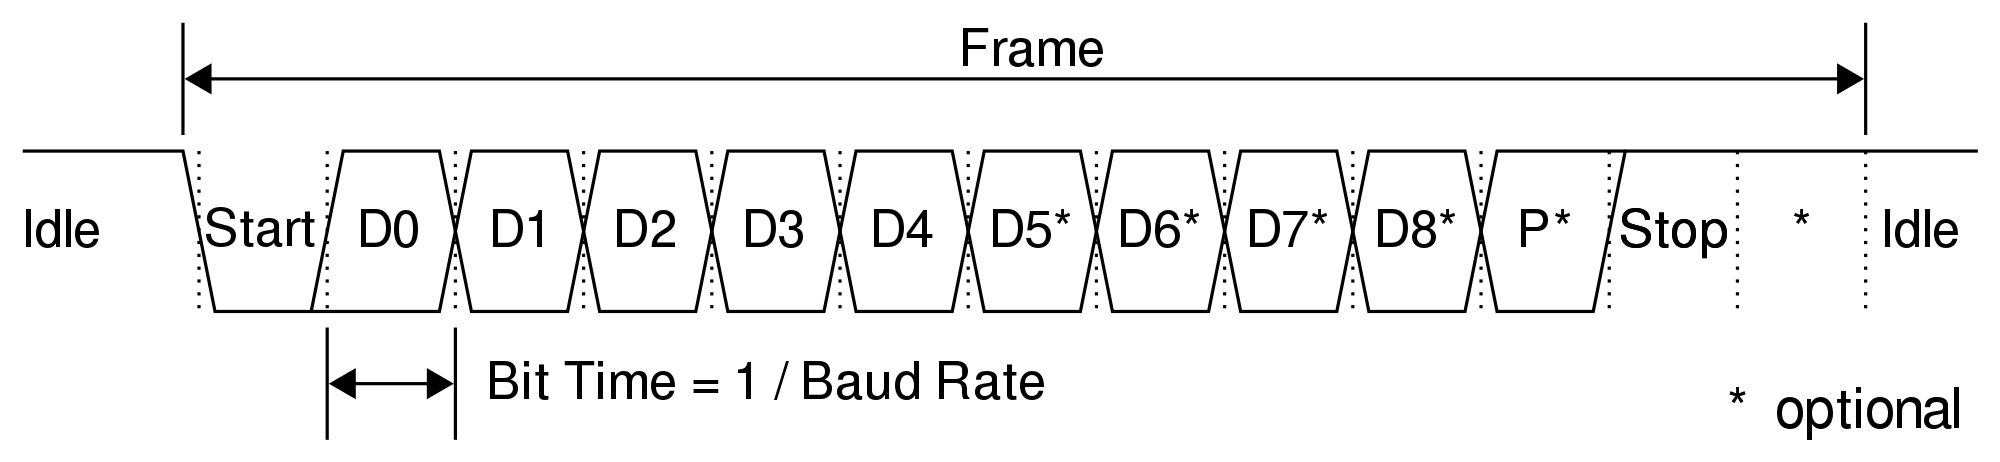
\includegraphics[width= \textwidth]{figures/UART.png}
                \caption{\label{figure:uart} Standard UART Frame}
            \end{center}
        \end{figure}

        In the NEORV32, to use the UART you should configure it, trough the CTRL register. First, you need to enable the UART, setting the UART\_CTRL\_EN. Then, the baud rate is configured, to be able to communicate with another device. The Baud rate is configured via UART\_CTRL\_BAUDx baud[9:0] (baud\_div + 1) and UART\_CTRL\_PRSC[2:0] (clock\_prescaler). Then, the frequency is going to be defined as presented in \autoref{eq:uart}. Furthermore, to read or write data, it is necessary to read or write to the UART\_DATA\_RTX\_*, which is the buffer that stores the Rx and Tx data.

        \begin{equation}
            Baud rate = \frac{fmain}{clock\_prescaler} \cdot \frac{1}{baud\_div + 1}
            \label{eq:uart}
        \end{equation}

        Additionally, it could be mentioned that it is possible to use two channels, UART0 and UART1. Both channels work in the same way. But the priority of channel 0 and 1 are different, as previously shown in \autoref{fig:firqs}.

        \newpage

        \begin{table}[!ht]
        	\centering
        	\caption{UART's memory-mapped registers.}
        	\adjustbox{max width=\textwidth}{
        		\begin{tabular}{ccp{7cm}cp{3cm}}
        			\toprule
        			\textbf{Address} & \textbf{Name [C]} & \textbf{(Bits)Name [C]} & \textbf{R/W} & \textbf{Function} \\
        			\midrule
        			\midrule
        			0xFFFFFFA0 & CTRL & (0)UART\_CTRL\_EN & r/w & UART enable \\
        			& & (1)UART\_CTRL\_SIM\_MODE & r/w & Enable simulation mode \\
        			& & (2)UART\_CTRL\_HWFC\_EN & r/w & Enable RTS/CTS hardware flow-control \\
        			& & (5:3)UART\_CTRL\_PRSC[2:0] & r/w & Baud rate clock prescaler select \\
        			& & (15:6)UART\_CTRL\_BAUD[9:0] & r/w & 12-bit Baud value configuration value \\
        			& & (16)UART\_CTRL\_RX\_NEMPTY & r/- & RX FIFO not empty \\
        			& & (17)UART\_CTRL\_RX\_HALF & r/- & RX FIFO at least half-full \\
        			& & (18)UART\_CTRL\_RX\_FULL & r/- & RX FIFO full \\
        			& & (19)UART\_CTRL\_TX\_EMPTY & r/- & TX FIFO empty \\
        			& & (20)UART\_CTRL\_TX\_NHALF & r/- & TX FIFO not at least half-full \\
        			& & (21)UART\_CTRL\_TX\_FULL & r/- & TX FIFO full \\
        			& & (22)UART\_CTRL\_IRQ\_RX\_NEMPTY & r/w & Fire IRQ if RX FIFO not empty \\
        			& & (23)UART\_CTRL\_IRQ\_RX\_HALF & r/w & Fire IRQ if RX FIFO at least half-full \\
        			& & (24)UART\_CTRL\_IRQ\_RX\_FULL & r/w & Fire IRQ if RX FIFO full \\
        			& & (25)UART\_CTRL\_IRQ\_TX\_EMPTY & r/w & Fire IRQ if TX FIFO empty \\
        			& & (26)UART\_CTRL\_IRQ\_TX\_NHALF & r/w & Fire IRQ if TX not at least half-full \\
        			& & (29:27)ZERO & r/- & Reserved, read as zero \\
        			& & (30)UART\_CTRL\_RX\_OVER & r/- & RX FIFO overflow \\
        			& & (31)UART\_CTRL\_TX\_BUSY & r/- & TX busy or TX FIFO not empty \\
                    \midrule
        			0xFFFFFFA4 & DATA & (7:0)UART\_DATA\_RTX\_* & r/w & Receive/Transmit data \\
        			& & (11:8)UART\_DATA\_RX\_FIFO\_SIZE\_* & r/- & log2(RX FIFO size) \\
        			& & (15:12)UART\_DATA\_TX\_FIFO\_SIZE\_* & r/- & log2(RX FIFO size) \\
        			  & Reserved & (31:16)ZERO & r/- & Reserved, read as zero \\
        			\bottomrule
        		\end{tabular}
        	}
        	\label{tab:uart_registers}
        \end{table}

        \subsection{UART interface}

            To use the UART in the development board, it is used the J6, a RS-232 connector. And a IC makes the conversion of RS-232 to UART, as presented in \autoref{fig:uart_development_board}.  
            
            \begin{figure}[!ht]
                \begin{center}
                    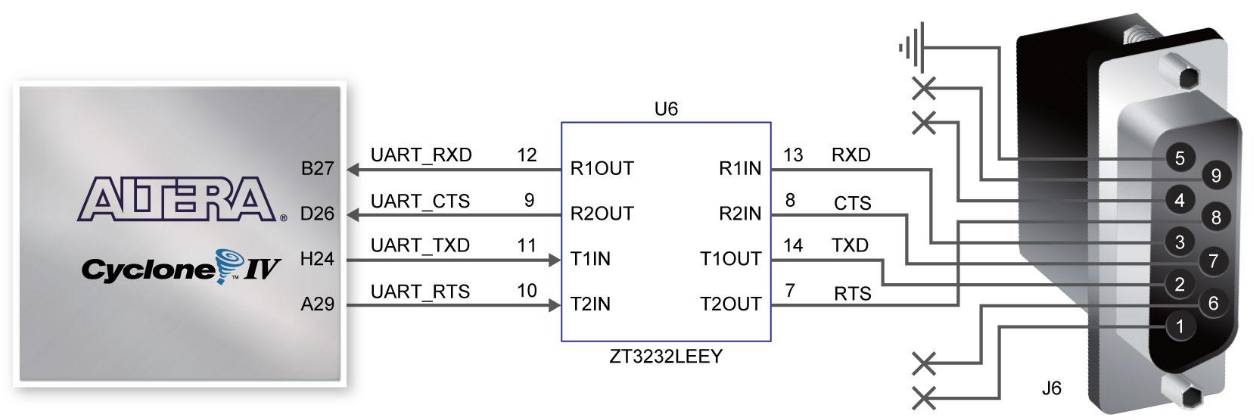
\includegraphics[width= 0.6\textwidth]{figures/uart_development_board.png}
                    \caption{\label{fig:uart_development_board} UART interface in the development board.}
                \end{center}
            \end{figure} % presents the peripherals and the board 
    %f
% programming.tex
%
% Copyright (C) 2023 UFSC.
%
% DOCUMENTATION-TEMPLATE
%
% This work is licensed under the Creative Commons Attribution-ShareAlike 4.0
% International License. To view a copy of this license,
% visit http://creativecommons.org/licenses/by-sa/4.0/.
%



\chapter{Recording to the FPGA's Internal Memory} \label{chp:chapter_rec}

    The \autoref{chp:chapter_rec} aims helping the laboratory's technician to properly configure the development board. We will first explain how to upload permanently the NEORV32, described in VHDL, to the development board.

    Then, we need to ensure that the NEORV32's toolchain is properly installed in the laboratory's computers. This toolchain provides a collection of software tools required for developing applications specifically designed for the NEORV32 processor. So, the process of downloading and installing the toolchain on the system will be presented in the following subsections:

    \autoref{sec:section_rec.1}:
    First, in this section you will find a guide on how to record the NEORV32 to the FPGA's internal memory using Intel's software, Quartus.
        
    \autoref{sec:section_rec.2}:
    Finally, we have a tutorial on how downloading and installing the toolchain.
    
    \section{Step by step to record in internal memory} \label{sec:section_rec.1}
    
        First, open the .sof to .pof (programming object file) converter. To do that, you should go to File > Convert Programming Files. Then you will have access to the window presented in \autoref{fig:f1}).

            \begin{figure}[!ht]
                \begin{center}
                    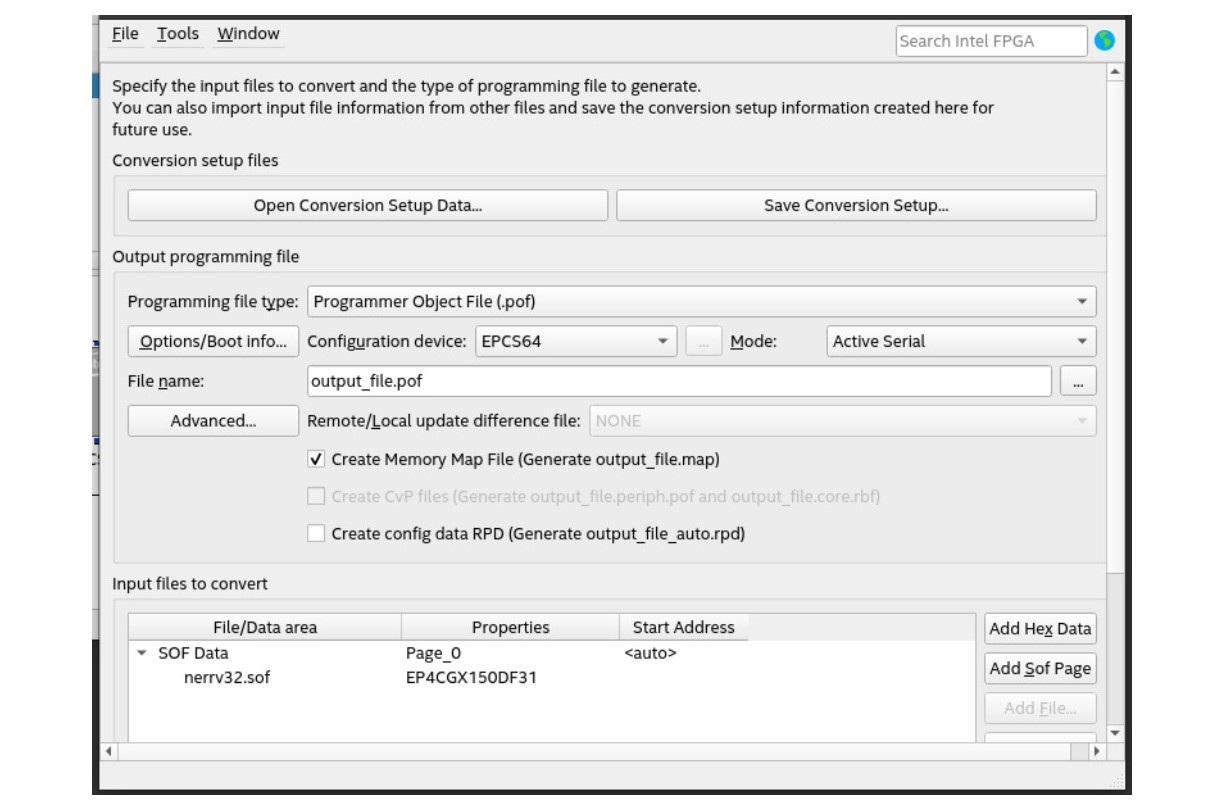
\includegraphics[width= 0.8\textwidth]{figures/chap2/fpga1.jpg}
                    \caption{\label{fig:f1} Convert Programming Files Tool.}
                \end{center}
            \end{figure}        
            
        Then, on the development board switch to the recording mode (PROG) using the ``programming mode switch'', shown in the \autoref{fig:f2}.
        
            \begin{figure}[!ht]
                \begin{center}
                    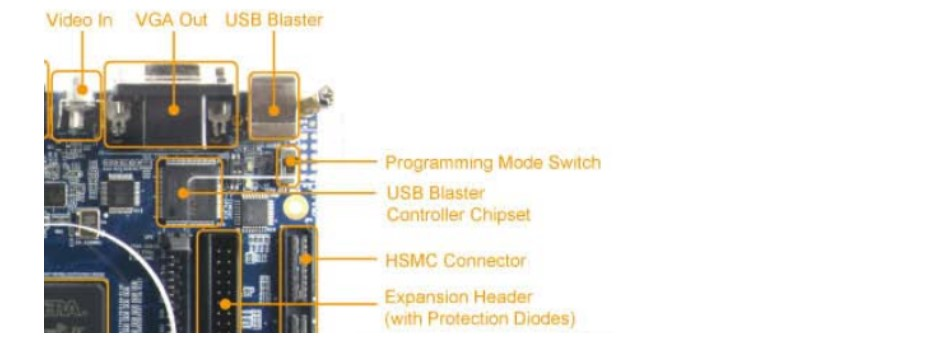
\includegraphics[width= 0.7\textwidth]{figures/chap2/fpga2.jpg}
                    \caption{\label{fig:f2} Programming Switch Indication.}
                \end{center}
            \end{figure}
        
        Next, on Quartus II, go to Tools > Programmer.
            
            \begin{figure}[!ht]
                \begin{center}
                    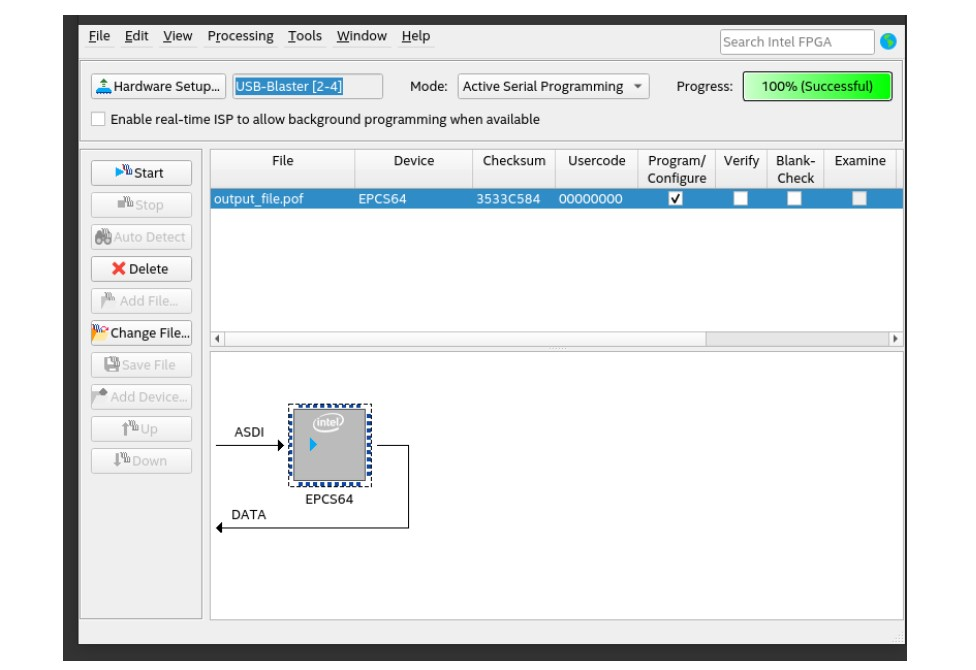
\includegraphics[width= 0.8\textwidth]{figures/chap2/fpga3.jpg}
                    \caption{\label{fig:f3} Programmer Tool.}
                \end{center}
            \end{figure}
        
        Finally, set the mode to ``active serial programming'', add the .pof file and click start, as presented in \autoref{fig:f3}. Before starting the development board, return the mode to ``run''.

        \section{Downloading and installing the toolchain} \label{sec:section_rec.2}
    
            First, you should access \url{https://github.com/stnolting/riscv-gcc-prebuilt}, to download the most recent available toolchain (today, \today, \textcolor{blue}{\textbf{rv32i-4.0.0}}). You should have now access to a .tar.gz file. Then, the next step, is to create the folder that the toolchain is going to be installed. You can open a terminal and type:
            
                \begin{lstlisting}[style=mystyle_bash, language=bash]
                    $ sudo mkdir /opt/riscv
                \end{lstlisting}
            
            Now, you need to navigate to the folder where the .tar.gz file was downloaded, like:
            
                \begin{lstlisting}[style=mystyle_bash, language=bash]
                    $ cd Downloads/
                \end{lstlisting}
                
            And then you have to extract the .tar.gz file to the folder previously created:
            
                \begin{lstlisting}[style=mystyle_bash, language=bash]
                    $ sudo tar -xzf <toolchain_version>.tar.gz -C /opt/riscv/
                \end{lstlisting}
                
            Finally, you should add the toolchain's bin folder to your system's PATH environment variable. You can open the .bashrc file:
            
                \begin{lstlisting}[style=mystyle_bash, language=bash]
                    $ sudo nano .bashrc
                \end{lstlisting}
                
            And then add the following line in the end of the .bashrc file:
            
                \begin{lstlisting}[style=mystyle_bash, language=bash]
                    export PATH="/opt/riscv/bin:$PATH"
                \end{lstlisting}
                
            To make sure everything works fine, navigate to the folder with the aplication examples and execute the following command:
            
                \begin{lstlisting}[style=mystyle_bash, language=bash]
                    $ make check
                \end{lstlisting}
            
            If everything is working fine you should se an ``\textbf{OK}'' appearing at the end, like in the \autoref{fig:successful_check}.
            
                \begin{figure}[!ht]
                    \begin{center}
                        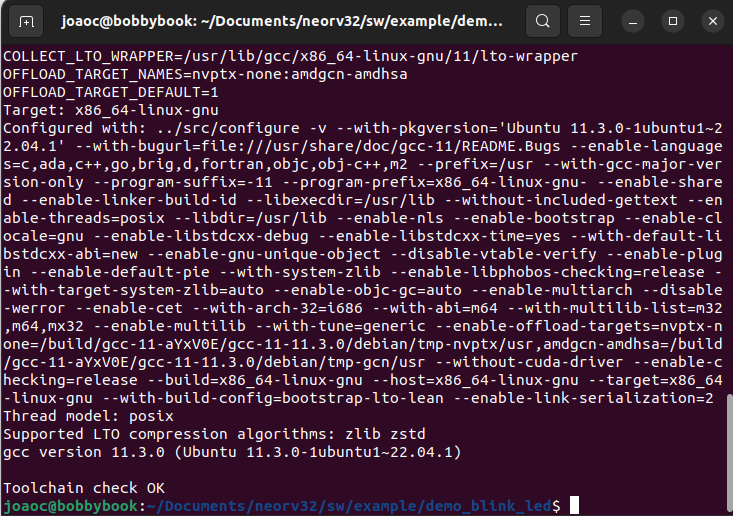
\includegraphics[width= 0.6\textwidth]{figures/successful_check.png}
                        \caption{Indication that the installation was successful.}
                        \label{fig:successful_check}
                    \end{center}
                \end{figure}
        

\chapter{Compiling and executing your first program} \label{ch:chapter_comp}

    Now, we will explore the process of compiling and executing your first program using the NEORV32's toolchain. This chapter aims to guide you through the necessary steps to successfully compile and run programs on the NEORV32.
    
    \autoref{sec:section_comp.1}: In this section, we will explore the process of flashing the compiled program into the FPGA board using the NEORV32 bootloader. The bootloader serves as an intermediary step between the development environment and the execution of the program on the FPGA board. We will guide you through the steps required to configure a terminal emulator, communicate with the FPGA board, and upload the program for execution.
    
    \autoref{sec:section_comp.2}: In addition to using the bootloader, we will also discuss an alternative method for flashing programs directly onto the FPGA board. This approach servers only to those that want to try something different, but it is no recommended using it during the course. It involves generating a VHDL file (.vhd) that represents the application code to be stored in the Instruction Memory (IMEM) of the NEORV32 processor. We will explain how to generate the .vhd file and integrate it into your project, either by replacing the existing application file or adding it to the project if it does not already exist.
    
    By understanding the process of compiling and executing programs on the NEORV32 processor and FPGA board, both you and your students will gain valuable practical experience in working with embedded systems. So, let's dive into the exciting world of FPGA programming and explore the possibilities offered by the NEORV32 toolchain!
    
    
    
        %\subsection{Some important commands}
        
        %Now that the toolchain was installed, you should know some commands to generate the .hex, .bin, .vdh, as well as other types of files. As you can see in \autoref{fig:toolchain_commands}, you could use \texttt{\hl{hex}} to generate the .hex file, which represents the machine language. You could use, for instance, the \texttt{\hl{image}} to generate the .vhd file, which is used to generate the \textit{neor32\_application\_image.vhd} that stores the main program that will run in the microprocessor. 
        
        
        %\begin{figure}[!ht]
        %    \begin{center}
        %        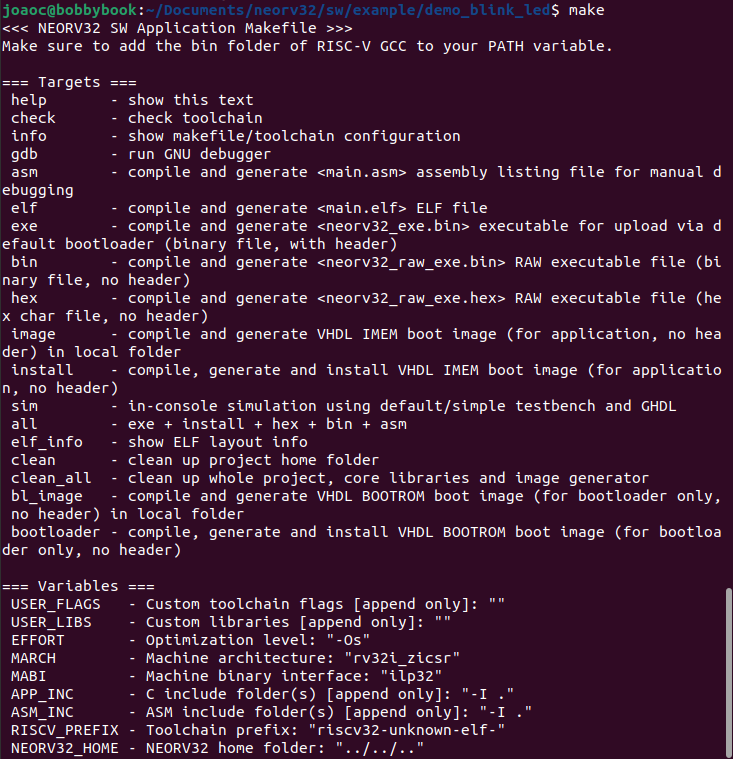
\includegraphics[width= 0.6\textwidth]{figures/toolchain_commands.png}
        %        \caption{Some useful commands to use.}
        %        \label{fig:toolchain_commands}
        %    \end{center}
        %\end{figure}
        
    \section{Flash the program into FPGA Board using bootloader} \label{sec:section_comp.1}
    
        In Linux, you should install a terminal emulator, like Minicom, Cutecom or similar:
        
            \begin{lstlisting}[style=mystyle_bash, language=bash]
                $ sudo apt install cutecom
            \end{lstlisting}
        
        Then the software should be configured like in \autoref{fig:cutecom_configuration}.  With the FPGA previously programmed with the base of the NEORV32, you should see the status LED (LDEG[0]) starts blinking and the bootloader intro screen appearing in your console, like:
        
            \begin{lstlisting}[style=mystyle_bash, language=bash]
                << NEORV32 Bootloader >>
            
                BLDV: Mar  7 2023
                HWV:  0x01080107
                CID:  0x00000000
                CLK:  0x05f5e100
                MISA: 0x40901106
                XISA: 0xc0000fab
                SOC:  0xffff402f
                IMEM: 0x00008000 bytes @0x00000000
                DMEM: 0x00002000 bytes @0x80000000
            
                Autoboot in 8s. Press any key to abort.
            \end{lstlisting}
            
            \begin{figure}[!ht]
                \begin{center}
                    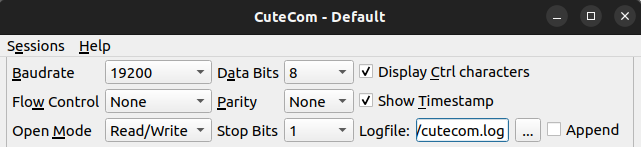
\includegraphics[width= 0.6\textwidth]{figures/cutecom_configuration.png}
                    \caption{Cutecom configuration.}
                    \label{fig:cutecom_configuration}
                \end{center}
            \end{figure}
            
        Now you can press any key to abort the automatic boot sequence and to start the actual bootloader user interface console. You then will have access to some commands, like:
        
            \begin{lstlisting}[style=mystyle_bash, language=bash]
                Available CMDs:
                h: Help
                r: Restart
                u: Upload
                s: Store to flash
                l: Load from flash
                x: Boot from flash (XIP)
                e: Execute
            \end{lstlisting}
        
        You can now upload the .bin file to execute it in the NEORV32. First you should create this file, by going to your application's folder and compiling it: 
        
            \begin{lstlisting}[style=mystyle_bash, language=bash]
                $ make clean_all exe
            \end{lstlisting}
    
        This command will create the \textit{neorv32\_exe.bin} file, which you will send to the FPGA. Then click on the \textit{send file} option to select the correct file. Finally, you can execute the program.
        
    \section{Flash the program into FPGA board directly} \label{sec:section_comp.2}
        
        To generate an .vhd file for the IMEM that contains the actual application, run the \texttt{\hl{image}} inside the folder of your application. For instance, you could use any application from the NEORV32's examples folder, like neorv32-setup/sw/exmaple/demo\_blink\_led:
        
            \begin{lstlisting}[style=mystyle_bash, language=bash]
                $ make clean_all image
            \end{lstlisting}
        
        This command will create the \textit{neorv32\_application\_image.vhd} file, that you can then add to the project's folder. If you are using Quartus II, you could replace the current application file or add it to the project if don't exists already. % chapter for the technician
    %
% examples.tex
%
% Copyright (C) 2023 UFSC.
%
% DOCUMENTATION-TEMPLATE
%
% This work is licensed under the Creative Commons Attribution-ShareAlike 4.0
% International License. To view a copy of this license,
% visit http://creativecommons.org/licenses/by-sa/4.0/.
%         
    
\chapter{High-level examples}\label{chp:chapter_ex}

    Welcome to the chapter that will help you put into practice all the lessons you have learned so far. Here you will find some high-level examples. It is important to point out that the code that you are going to develop during the course won't have pre-built functions. So, you are going to develop low-level code. All code is written in C, so we hope you have already read the previous chapters to understand how to handle all the NEORV32's registers, as well as to programming in C.

    \autoref{sec:section_ex.1}:
    In this section we have an example of a GPIO implementation in the NEORV32.
        
    \autoref{sec:section_ex.2}:
    In this section we have an example of a 7-segment display implementation in the NEORV32.

    \autoref{sec:section_ex.2}:
    In this section we have an example of a 7-segment display implementation in the NEORV32.

    \autoref{sec:section_ex.3}:
    In this section we have an example of a LCD display implementation in the NEORV32.

    \autoref{sec:section_ex.4}:
    In this section we have an example of a interrupts implementation in the NEORV32.
    
    \autoref{sec:section_ex.5}:
    In this section we have an example of a timer/counter implementation in the NEORV32.

    \autoref{sec:section_ex.5}:
    In this section we have an example of a serial UART implementation in the NEORV32.

    \section{GPIO}\label{sec:section_ex.1}

        In this section \autoref{sec:section_ex.1} we will understand a simple example of using a GPIO.
        The idea of the implementation is to make a counter using the red LEDs starting from LEDR[7] to LEDR[0], and as seen in \autoref{sec:section_ex.1} we only have 8 pins available for red LEDs.

    
        \begin{lstlisting}[style=mystyle_c, language=c, breaklines]
            /************************************************************//**
             * @file demo_blink_led/main.c
             * @author J.C.E. Barcellos
             * @brief A simple GPIO application.
             ***************************************************************/
            #include <neorv32.h>
            /************************************************************//**
             * @brief Shows an incrementing 8-bit counter on LEDR[7..0].
             *
             * @note This program requires the GPIO controller to be synthesized.
             *
             * @return Will never return.
             ***************************************************************/
            int main() {
            
            	int cnt = 0; // counter
            	
            	while (1) {
            		neorv32_gpio_port_set((cnt++ & 0xFF) << 9); // increment counter and mask for lowest 8 bits
            		neorv32_cpu_delay_ms(500); // wait 500ms
            	}
            	
            	return 0; // this should never be reached
            }
    \end{lstlisting}

    So let's start with a declaration of the variable ``cnt'', with initial data of 0. 
    
    Further down in a while loop we use the function ``neorv32\_gpio\_port\_set()'' from the GPIO library to link the parameter to the output (the LEDs). In this case, the parameter of this function will be the variable ``cnt'' being incremented, plus a logical AND operation with 0xFF (which in binary would be ``11111111''), all being shifted 9 bits.
   
    Now let's understand what this all means: 
    \& 0xFF would be a mask created for cnt, where only the 8 LSB bits are used. When these 8-bit values resulting from the mask are dumped into port\_set, the green LEDs will turn on instead of the red ones, but why does this happen? This is due to the fact that the GPIO\_o pins start with LEDGs that go from bit 0 to 8 (available in \autoref{tab:ledg_o}), so it is necessary to shift 9 bits so that the red LEDs to be set.
    
    \section{7-segment Display} \label{sec:section_ex.2}

        In this section \autoref{sec:section_ex.2} we will learn how to implement a 7-segment display. Make it display values from '0' to 'F' periodically. 

            \begin{lstlisting}[style=mystyle_c, language=c, breaklines]
                /************************************************************//**
                 * @file demo_lcd/main.c
                 * @author J.C.E. Barcellos
                 * @brief A simple 7-segment display application.
                 ***************************************************************/
                #include <neorv32.h>
                #include <stdint.h>
                #include <stdio.h>
                #include <string.h>
                /************************************************************//**
                 * @brief Prints 0 to 15 in hex format into the 7-segment display.
                 *
                 * @note This program requires the GPIO controller to be synthesized.
                 *
                 * @return Will never return.
                 ***************************************************************/
                int main() {
                
                	char display_chars[] = "0123456789ABCDEF"; // characters to be displayed in sequence
                	int num_chars = sizeof(display_chars) - 1; // -1 to exclude the null terminator
                
                	while (1) {
                		for (int i = 0; i < num_chars; i++) {
                			neorv32_display_write(CHANNEL_0, &display_chars[i]); // display each charater to the 7-segment display
                			neorv32_cpu_delay_ms(500); // wait 1s
                		}
                		neorv32_display_clear(CHANNEL_0); // clears the 7-segment display
                		neorv32_cpu_delay_ms(2000); // wait 2s
                	}
                
                	return 0; // this should never be reached
                }       
        \end{lstlisting}

        Now we are going to implement a 7-segment display. We create a variable of type character, ``display\_chars'' which will be our sequence of characters that will be shown on the display. Another variable will be of type integer which will be the size of the variable ``display\_chars'' - 1, being the maximum bit the sequence will have.
    
        The function ``neorv32\_display\_write()'' will be responsible for sending the character to a converter and then to the display. The first parameter will be in charge of shifting the character to the pin available for the 7-segment display, in the case of CHANNEL\_0, it will be a 16-bit shift. And so, each increment of ``i'' and each character of display\_chars[] will be sent to the display.
        
        Finally, the display will be cleared as soon as ``i'' is bigger than ``num\_chars'' and a delay of 2000 ms will be executed.
        
        Remember that you can see any details about the functions of the library responsible for the LCD Display at \autoref{.c:-7-segments} and \autoref{.h:7-segments}.

            
    \section{LCD Display} \label{sec:section_ex.3}

        In this section \autoref{sec:section_ex.3} we will learn how to implement an LCD Display. The goal is simple, write a message and have it appear on the display.

            \begin{lstlisting}[style=mystyle_c, language=c, breaklines]
                /************************************************************//**
                 * @file demo_lcd/main.c
                 * @author J.C.E. Barcellos
                 * @brief A simple LCD application.
                 ***************************************************************/
                #include <neorv32.h>
                #include <stdint.h>
                #include <stdio.h>
                #include <string.h>
                /************************************************************//**
                 * @brief Prints a series of sentences into the LCD.
                 *
                 * @note This program requires the GPIO controller to be synthesized.
                 *
                 * @return Will never return.
                 ***************************************************************/
                int main() {
                
                	// turn on the LCD with a blinking cursor
                	neorv32_lcd_display_on(); 
                
                	// writes the first sentence to the LCD
                	neorv32_lcd_write("Hello, guys!"); 
                	neorv32_cpu_delay_ms(2000);
                
                	// clear the LCD and return the cursor to its origin
                	neorv32_lcd_clear_display(); 
                	neorv32_lcd_return_to_origin(); 
                	neorv32_cpu_delay_ms(2000);
                
                	// writes the second and last sentence to the LCD
                	neorv32_lcd_write("How are you?"); 
                
                	// go to sleep mode
                    while(1) {
                        neorv32_cpu_sleep();
                    }
                	
                	return 0; // this should never be reached
                }        
        \end{lstlisting}

            We will start the code turn on the LCD display with the function ``neorv32\_lcd\_display\_on()''. Next we will use ``neorv32\_lcd\_write()'' to convert the chosen message into a character and write it to the LCD display. So when we are done sending the message we need to clear the LCD and return the cursor to origin with the respective functions: ``neorv32\_lcd\_clear\_display()'' and ``neorv32\_lcd\_return\_to\_origin()''. Then it will write a message again and go into sleep mode.
            Remember that you can see any details about the functions of the library responsible for the LCD Display at \autoref{.c:lcd} and \autoref{.h:lcd}.
    
    \section{Interrupts} \label{sec:section_ex.4}
    
        In this section \autoref{sec:section_ex.4} we learned about interrupts and now make an external interrupt controller using the libraries available in neorv32.

            \begin{lstlisting}[style=mystyle_c, language=c, breaklines]
                /************************************************************//**
                 * @file demo_xirq/main.c
                 * @author J.C.E. Barcellos
                 * @brief A simple external interruption application.
                 ***************************************************************/
                #include <neorv32.h>
                #include <string.h>
                
                // defines
                #define LEDR_0 0x09
                
                /************************************************************//**
                 * @brief XIRQ handler.
                 ***************************************************************/
                void button_xirq_handler(void) {
                    neorv32_gpio_pin_toggle(LEDR_0); // toggle the LEDR[0]
                }
                
                /************************************************************//**
                 * @brief Toggles a LED every every time a button is pressed.
                 *
                 * @note This program requires the XIRQ and the GPIO controller to be synthesized.
                 *
                 * @return Will never return.
                 ***************************************************************/
                int main() {
                
                    // initialize the runtime environment, to handling all CPU's traps
                    neorv32_rte_setup();
                
                    // check if XIRQ controller was synthesized.
                    if (neorv32_xirq_available() == 0) {
                        neorv32_gpio_pin_set(0x01);
                    }
                
                    // initialize the XIRQ controller
                    if (neorv32_xirq_setup() != 0) {
                        neorv32_gpio_pin_set(0x02);
                    }
                
                    // install handler functions for XIRQ 
                    if (neorv32_xirq_install(0, button_xirq_handler) != 0) {
                        neorv32_gpio_pin_set(0x03);
                    }
                
                    // enable XIRQ interrupts
                    neorv32_xirq_global_enable();
                
                    // enable machine-mode interrupts
                    neorv32_cpu_csr_set(CSR_MSTATUS, 1 << CSR_MSTATUS_MIE);
                
                    while(1){
                        neorv32_cpu_sleep();
                    }
                
                    return 0;
                }        
        \end{lstlisting}

        We will start by adding a ``define'' with the LEDR that is responsible for lighting up when there is an interruption and this will be included in a function that links this LEDR with a GPIO.
        So next we use the function ``neorv32\_rte\_setup'' to initialize the runtime environment. We check if the interrupt controller is synthesized. If so we set ``neorv32\_gpio\_pin\_set(0x01)'' in the GPIO.  Also if the controller is not initialized we set ``neorv32\_gpio\_pin\_set(0x02)'' to initialize it. We install the handler functions for XIRQ by setting ``neorv32\_gpio\_pin\_set(0x03)''. To make the handlers interrupt enable ``neorv32\_xirq\_global\_enable()''. Then we make machine-mode interrupts enable. 
        Remember that every library responsible for XIRQ can be found in the neorv32 files.
    
    \section{Timer/Counter} \label{sec:section_ex.5}

            In this section \autoref{sec:section_ex.5} we learned about timers/counters and now in a similar way to the external interrupt controller, so make a timer/counter application, with 1 second delay and using the libraries available in neorv32.

            \begin{lstlisting}[style=mystyle_c, language=c, breaklines]
                /************************************************************//**
                 * @file demo_mtime/main.c
                 * @author J.C.E. Barcellos
                 * @brief A simple timer application.
                 ***************************************************************/
                #include <neorv32.h>
                
                // defines
                #define DELAY_S 1
                
                /************************************************************//**
                 * @brief MTIME IRQ handler.
                 ***************************************************************/
                void mtime_irq_handler(void) {
                    static int cnt = 0; // counter
                
                    // update the time for the next interrupt
                    neorv32_mtime_set_timecmp(neorv32_mtime_get_timecmp() + DELAY_S*(NEORV32_SYSINFO->CLK / 2));
                
                    // increment counter and mask for lowest 8 bits
                	neorv32_gpio_port_set((cnt++ & 0xFF)<<9); 
                }
                
                /************************************************************//**
                 * @brief increments a 8-bit counter on LEDR[7..0] using the machine timer interrupt.
                 *
                 * @note This program requires the MTIME and the GPIO controller to be synthesized.
                 *
                 * @return Will never return.
                 ***************************************************************/
                int main() {
                
                    // initialize the runtime environment, to handling all CPU's traps
                    neorv32_rte_setup();
                
                    // check if MTIME controller was synthesized.
                    if (neorv32_mtime_available() == 0) {
                        neorv32_gpio_pin_set(0x01);
                    }
                
                    // install handler functions for MTIME 
                    if (neorv32_rte_handler_install(RTE_TRAP_MTI, mtime_irq_handler) != 0) {
                        neorv32_gpio_pin_set(0x02);
                    }
                
                    // configure the time for the first interrupt
                    neorv32_mtime_set_timecmp(neorv32_mtime_get_time() + DELAY_S*(NEORV32_SYSINFO->CLK / 2));
                
                    // enable interrupt
                    neorv32_cpu_csr_set(CSR_MIE, 1 << CSR_MIE_MTIE); // enable MTIME interrupt
                    neorv32_cpu_csr_set(CSR_MSTATUS, 1 << CSR_MSTATUS_MIE); // enable machine-mode interrupts
                
                    // go to sleep mode
                    while(1) {
                        neorv32_cpu_sleep();
                    }
                
                    return 0; // this should never be reached
                }            
        \end{lstlisting}

        For the timer/counter we set a delay. We create a function responsible for controlling the timer ``MTIME IRQ'' that will update the time for the next interrupt and increment the counter to the least significant 8 bits.

        In the main we start the runtime environment, to handle all CPU's traps, we check if the controller is synthesize. We install the handler functions for MTIME and set the time for the first interrupt, making the time now plus 1 second ((NEORV32\_SYSINFO->CLK / 2) is equal to 1). We make the interrupt enable and the machine-mode interrupts. 


    
    \section{Serial UART} \label{sec:section_ex.6}

        In this section \autoref{sec:section_ex.6} we learned about UART and now do the application using UART, that when we send a certain message, we will receive a specific message back from the microprocessor.

            \begin{lstlisting}[style=mystyle_c, language=c, breaklines]
                /************************************************************//**
                 * @file demo_uart/main.c
                 * @author J.C.E. Barcellos
                 * @brief A simple UART application.
                 ***************************************************************/
                #include <neorv32.h>
                #include <stdio.h>
                #include <string.h>
                
                // defines
                #define BAUD_RATE 19200
                
                // prototypes
                void uart_irq_handler(void);
                
                /************************************************************//**
                 * @brief Every time it receives the question "Are you alright?" it will respond with "I'm alive".
                 *
                 * @note This program requires the UART and the GPIO controller to be synthesized.
                 *
                 * @return Will never return.
                 ***************************************************************/
                int main() {
                
                    char buffer[50]; // buffer for the received message
                
                    // initialize the UART with default baud rate
                    neorv32_uart0_setup(BAUD_RATE, 0);
                
                    // initialize the runtime environment, to handling all CPU's traps
                    neorv32_rte_setup();
                
                    // check if UART controller was synthesized.
                    if (neorv32_uart0_available() == 0) {
                        neorv32_gpio_pin_set(0x01);
                    }
                
                
                    while(1) {
                        // send a message for the user and waits for a response
                        neorv32_uart0_printf("Hi! \n");
                        neorv32_uart0_scan(buffer, 50, 1);
                        neorv32_uart0_printf("\n");
                
                        // compares the response with the expected one
                        if (!strcmp(buffer, "Are you alright?")) {
                            neorv32_uart0_printf("\n I'm alive! \n");
                            neorv32_uart0_printf("=) \n");
                            neorv32_uart0_printf("NEORV32 left the conversation... \n");
                        }
                
                        // go to sleep mode
                        // but you could remove it, to start a new interaction
                        while(1) {
                            neorv32_cpu_sleep();
                        }
                    }
                
                    return 0; // this should never be reached
                }
        \end{lstlisting}

        First, a buffer is created for incoming messages. We will start the UART with the usual settings and also the runtime environment, to handle all CPU's traps. We check if the UART is synthesized. So we print out a message and send it to the UART via ``neorv32\_uart0\_scan(buffer, 50, 1)''. If the message is ``Are you alright?'' the microprocessor will reply ``I'm alive!'' and ``NEORV32 left the conversation... ''.
        And finally it goes into sleep mode unless you want to start a new interaction.
        
    

 % show high-level examples 
    %
% references.tex
%
% Copyright (C) 2023 UFSC.
%
% DOCUMENTATION-TEMPLATE
%
% This work is licensed under the Creative Commons Attribution-ShareAlike 4.0
% International License. To view a copy of this license,
% visit http://creativecommons.org/licenses/by-sa/4.0/.
%
\bibliography{references/references.bib}

\addcontentsline{toc}{chapter}{References}
 % some references
    %
% appendices.tex
%
% Copyright (C) 2023 UFSC.
%
% DOCUMENTATION-TEMPLATE
%
% This work is licensed under the Creative Commons Attribution-ShareAlike 4.0
% International License. To view a copy of this license,
% visit http://creativecommons.org/licenses/by-sa/4.0/.
%

\begin{appendices}

%
% fpga_pinout.tex
%
% Copyright (C) 2023 UFSC.
%
% DOCUMENTATION-TEMPLATE
%
% This work is licensed under the Creative Commons Attribution-ShareAlike 4.0
% International License. To view a copy of this license,
% visit http://creativecommons.org/licenses/by-sa/4.0/.
%


\chapter{FPGA Output GPIO Pinout}

\begin{table}[!htb]\scriptsize
    \centering
    \begin{tabular}{c c c c}
        \toprule[1.5pt]
        \textbf{Type} & \quad \quad \textbf{NEORV32 PIN} & \quad \quad \textbf{FPGA Pin} & \quad \quad \textbf{Signal Name}  \\
          
        \midrule
               & \quad \quad GPIO\_o [0] & \quad \quad PIN\_AA25 & \quad \quad LEDG [0]\\
               & \quad \quad GPIO\_o [1] & \quad \quad PIN\_AB25 & \quad \quad LEDG [1]\\
               & \quad \quad GPIO\_o [2] & \quad \quad PIN\_F27  & \quad \quad LEDG [2]\\
        LEDG   & \quad \quad GPIO\_o [3] & \quad \quad PIN\_F26  & \quad \quad LEDG [3]\\        
               & \quad \quad GPIO\_o [4] & \quad \quad PIN\_W26  & \quad \quad LEDG [4]\\
               & \quad \quad GPIO\_o [5] & \quad \quad PIN\_Y22  & \quad \quad LEDG [5]\\
               & \quad \quad GPIO\_o [6] & \quad \quad PIN\_Y25  & \quad \quad LEDG [6]\\
               & \quad \quad GPIO\_o [7] & \quad \quad PIN\_AA22 & \quad \quad LEDG [7]\\
               & \quad \quad GPIO\_o [8] & \quad \quad PIN\_J25  & \quad \quad LEDG [8]\\
            \bottomrule[1.5pt]
         
    \end{tabular}
    \caption{\label{tab:ledg_o} Green LEDs pinout}
\end{table}


\begin{table}[!htb]\scriptsize
    \centering
    \begin{tabular}{c c c c}
        \toprule[1.5pt]
        \textbf{Type} & \quad \quad \textbf{NEORV32 PIN} & \quad \quad \textbf{FPGA Pin} & \quad \quad \textbf{Signal Name}  \\
        
               & \quad \quad GPIO\_o [9]  & \quad \quad PIN\_T23 & \quad \quad LEDR [0]\\
               & \quad \quad GPIO\_o [10] & \quad \quad PIN\_T24 & \quad \quad LEDR [1]\\
               & \quad \quad GPIO\_o [11] & \quad \quad PIN\_V27 & \quad \quad LEDR [2]\\
        LEDR   & \quad \quad GPIO\_o [12] & \quad \quad PIN\_W25 & \quad \quad LEDR [3]\\        
               & \quad \quad GPIO\_o [13] & \quad \quad PIN\_T21 & \quad \quad LEDR [4]\\
               & \quad \quad GPIO\_o [14] & \quad \quad PIN\_T26 & \quad \quad LEDR [5]\\
               & \quad \quad GPIO\_o [15] & \quad \quad PIN\_R25 & \quad \quad LEDR [6]\\
               & \quad \quad GPIO\_o [16] & \quad \quad PIN\_E15 & \quad \quad LEDR [7]\\

    \end{tabular}
    \caption{\label{tab:ledr_o}Red LEDs pinout}
\end{table}

\begin{table}[!htb]\scriptsize
    \centering 
    \begin{tabular}{c c c c}
        \toprule[1.5pt]
        \textbf{Type} & \quad \quad \textbf{NEORV32 PIN} & \quad \quad \textbf{FPGA Pin} & \quad \quad \textbf{Signal Name}  \\

               & \quad \quad GPIO\_o [16] & \quad \quad PIN\_E15 & \quad \quad HEX0 [0]\\
               & \quad \quad GPIO\_o [17] & \quad \quad PIN\_E12 & \quad \quad HEX0 [1]\\
               & \quad \quad GPIO\_o [18] & \quad \quad PIN\_G11 & \quad \quad HEX0 [2]\\
        HEX0   & \quad \quad GPIO\_o [19] & \quad \quad PIN\_F11 & \quad \quad HEX0 [3]\\        
               & \quad \quad GPIO\_o [20] & \quad \quad PIN\_F16 & \quad \quad HEX0 [4]\\
               & \quad \quad GPIO\_o [21] & \quad \quad PIN\_D16 & \quad \quad HEX0 [5]\\
               & \quad \quad GPIO\_o [22] & \quad \quad PIN\_F14 & \quad \quad HEX0 [6]\\
        \hline
               & \quad \quad GPIO\_o [23] & \quad \quad PIN\_G14 & \quad \quad HEX1 [0]\\
               & \quad \quad GPIO\_o [24] & \quad \quad PIN\_B13 & \quad \quad HEX1 [1]\\
               & \quad \quad GPIO\_o [25] & \quad \quad PIN\_G13 & \quad \quad HEX1 [2]\\
        HEX1   & \quad \quad GPIO\_o [26] & \quad \quad PIN\_F12 & \quad \quad HEX1 [3]\\        
               & \quad \quad GPIO\_o [27] & \quad \quad PIN\_G12 & \quad \quad HEX1 [4]\\
               & \quad \quad GPIO\_o [28] & \quad \quad PIN\_J9  & \quad \quad HEX1 [5]\\
               & \quad \quad GPIO\_o [29] & \quad \quad PIN\_G10 & \quad \quad HEX1 [6]\\    
        \hline
               & \quad \quad GPIO\_o [30] & \quad \quad PIN\_G8   & \quad \quad HEX2 [0]\\
               & \quad \quad GPIO\_o [31] & \quad \quad PIN\_G7   & \quad \quad HEX2 [1]\\
               & \quad \quad GPIO\_o [32] & \quad \quad PIN\_F7   & \quad \quad HEX2 [2]\\
        HEX2   & \quad \quad GPIO\_o [33] & \quad \quad PIN\_AG30 & \quad \quad HEX2 [3]\\        
               & \quad \quad GPIO\_o [34] & \quad \quad PIN\_F6   & \quad \quad HEX2 [4]\\
               & \quad \quad GPIO\_o [35] & \quad \quad PIN\_F4    & \quad \quad HEX2 [5]\\
               & \quad \quad GPIO\_o [36] & \quad \quad PIN\_F10  & \quad \quad HEX2 [6]\\  
        \hline
               & \quad \quad GPIO\_o [37] & \quad \quad PIN\_D10 & \quad \quad HEX3 [0]\\
               & \quad \quad GPIO\_o [38] & \quad \quad PIN\_D7  & \quad \quad HEX3 [1]\\
               & \quad \quad GPIO\_o [39] & \quad \quad PIN\_E6  & \quad \quad HEX3 [2]\\
        HEX3   & \quad \quad GPIO\_o [40] & \quad \quad PIN\_E4  & \quad \quad HEX3 [3]\\        
               & \quad \quad GPIO\_o [41] & \quad \quad PIN\_E3  & \quad \quad HEX3 [4]\\
               & \quad \quad GPIO\_o [42] & \quad \quad PIN\_D5  & \quad \quad HEX3 [5]\\
               & \quad \quad GPIO\_o [43] & \quad \quad PIN\_D4  & \quad \quad HEX3 [6]\\
               
        
    \end{tabular}
    \caption{\label{tab:hex}Display 7-segments pinout}
\end{table}

\begin{table}[!htb]\scriptsize
    \centering
    \begin{tabular}{c c c c}
        \toprule[1.5pt]
        \textbf{Type} & \quad \quad \textbf{NEORV32 PIN} & \quad \quad \textbf{FPGA Pin} & \quad \quad \textbf{Signal Name}  \\
          
        \midrule
                    & \quad \quad GPIO\_o [44] & \quad \quad PIN\_D22  & \quad \quad GPIO [0]\\
                    & \quad \quad GPIO\_o [45] & \quad \quad PIN\_D21  & \quad \quad GPIO [1]\\
                    & \quad \quad GPIO\_o [46] & \quad \quad PIN\_D23  & \quad \quad GPIO [2]\\
        GPIO Output & \quad \quad GPIO\_o [47] & \quad \quad PIN\_D24  & \quad \quad GPIO [3]\\        
                    & \quad \quad GPIO\_o [48] & \quad \quad PIN\_B28  & \quad \quad GPIO [4]\\
                    & \quad \quad GPIO\_o [49] & \quad \quad PIN\_C25  & \quad \quad GPIO [5]\\
                    & \quad \quad GPIO\_o [50] & \quad \quad PIN\_C26  & \quad \quad GPIO [6]\\
                    & \quad \quad GPIO\_o [51] & \quad \quad PIN\_D28  & \quad \quad GPIO [7]\\
            \bottomrule[1.5pt]
         
    \end{tabular}
    \caption{\label{tab:gpio_o}GPIO output pinout}
\end{table}

\begin{table}[!htb]\scriptsize
    \centering
    \begin{tabular}{c c c c}
        \toprule[1.5pt]
        \textbf{Type} & \quad \quad \textbf{NEORV32 PIN} & \quad \quad \textbf{FPGA Pin} & \quad \quad \textbf{Signal Name}  \\
        
               & \quad \quad GPIO\_o [52] & \quad \quad PIN\_AG4  & \quad \quad DATA [0]\\
               & \quad \quad GPIO\_o [53] & \quad \quad PIN\_AF3  & \quad \quad DATA [1]\\
               & \quad \quad GPIO\_o [54] & \quad \quad PIN\_AH3  & \quad \quad DATA [2]\\
               & \quad \quad GPIO\_o [55] & \quad \quad PIN\_AE5  & \quad \quad DATA [3]\\        
               & \quad \quad GPIO\_o [56] & \quad \quad PIN\_AH2  & \quad \quad DATA [4]\\
               & \quad \quad GPIO\_o [57] & \quad \quad PIN\_AE3  & \quad \quad DATA [5]\\
        LCD    & \quad \quad GPIO\_o [58] & \quad \quad PIN\_AH4  & \quad \quad DATA [6]\\  
               & \quad \quad GPIO\_o [59] & \quad \quad PIN\_AE4  & \quad \quad DATA [7]\\ 
               & \quad \quad GPIO\_o [60] & \quad \quad PIN\_AF4  & \quad \quad EN\\
               & \quad \quad GPIO\_o [61] & \quad \quad PIN\_AJ3  & \quad \quad RW\\
               & \quad \quad GPIO\_o [62] & \quad \quad PIN\_AG3  & \quad \quad RS\\
               & \quad \quad GPIO\_o [63] & \quad \quad PIN\_AF27 & \quad \quad ON\\
        \bottomrule[1.5pt]
    \end{tabular}
    \caption{\label{tab:lcd_o}LCD display pinout}
\end{table}

%%%%%%%%%%%%%%%%%%%%%%%%%%%%%%%%%%%%%%%%%%%%%%%%%%%%%%%%%%%%%%%%%%%%%%%%%%%%%%%%%%%%%%%%%%%%%%%%%%%%%%%%%

\chapter{FPGA Input GPIO Pinout}

\begin{table}[!htb]\scriptsize
    \centering
    \begin{tabular}{c c c c}
        \toprule[1.5pt]
        \textbf{Type} & \quad \quad \textbf{NEORV32 PIN} & \quad \quad \textbf{FPGA Pin} & \quad \quad \textbf{Signal Name}  \\
          
        \midrule
               & \quad \quad GPIO\_i [0] & \quad \quad PIN\_V28  & \quad \quad SW [0]\\
               & \quad \quad GPIO\_i [1] & \quad \quad PIN\_U30  & \quad \quad SW [1]\\
               & \quad \quad GPIO\_i [2] & \quad \quad PIN\_V21  & \quad \quad SW [2]\\
        SW     & \quad \quad GPIO\_i [3] & \quad \quad PIN\_C2   & \quad \quad SW [3]\\        
               & \quad \quad GPIO\_i [4] & \quad \quad PIN\_AB20 & \quad \quad SW [4]\\
               & \quad \quad GPIO\_i [5] & \quad \quad PIN\_U21  & \quad \quad SW [5]\\
               & \quad \quad GPIO\_i [6] & \quad \quad PIN\_T28  & \quad \quad SW [6]\\
               & \quad \quad GPIO\_i [7] & \quad \quad PIN\_IR30 & \quad \quad SW [7]\\
            \bottomrule[1.5pt]
         
    \end{tabular}
    \caption{\label{tab:sw_i}Switches pinout}
\end{table}

\begin{table}[!htb]\scriptsize
    \centering
    \begin{tabular}{c c c c}
        \toprule[1.5pt]
        \textbf{Type} & \quad \quad \textbf{NEORV32 PIN} & \quad \quad \textbf{FPGA Pin} & \quad \quad \textbf{Signal Name}  \\
          
        \midrule
                    & \quad \quad GPIO\_i [56] & \quad \quad PIN\_G16  & \quad \quad GPIO [0]\\
                    & \quad \quad GPIO\_i [57] & \quad \quad PIN\_F17  & \quad \quad GPIO [1]\\
                    & \quad \quad GPIO\_i [58] & \quad \quad PIN\_D18  & \quad \quad GPIO [2]\\
        GPIO Input  & \quad \quad GPIO\_i [59] & \quad \quad PIN\_F18  & \quad \quad GPIO [3]\\        
                    & \quad \quad GPIO\_i [60] & \quad \quad PIN\_D19  & \quad \quad GPIO [4]\\
                    & \quad \quad GPIO\_i [61] & \quad \quad PIN\_K21  & \quad \quad GPIO [5]\\
                    & \quad \quad GPIO\_i [62] & \quad \quad PIN\_F19  & \quad \quad GPIO [6]\\
                    & \quad \quad GPIO\_i [63] & \quad \quad PIN\_K22  & \quad \quad GPIO [7]\\

            \bottomrule[1.5pt]
         
    \end{tabular}
    \caption{\label{tab:gpio_i}Input GPIO pinout}
\end{table}

%%%%%%%%%%%%%%%%%%%%%%%%%%%%%%%%%%%%%%%%%%%%%%%%%%%%%%%%%%%%%%%%%%%%%%%%%%%%%%%%%%%%%%%%%%%%%%%%%%%%%%%%%

\chapter{FPGA Interrupts Pinout}

\begin{table}[!htb]\scriptsize
    \centering
    \begin{tabular}{c c c c}
        \toprule[1.5pt]
        \textbf{Type} & \quad \quad \textbf{NEORV32 PIN} & \quad \quad \textbf{FPGA Pin} & \quad \quad \textbf{Signal Name}  \\
          
        \midrule
                    & \quad \quad xirq\_i [0]  & \quad \quad PIN\_AE25  & \quad \quad KEY [1]\\
                    & \quad \quad xirq\_i [1]  & \quad \quad PIN\_AF30  & \quad \quad KEY [2]\\
        Interrupts  & \quad \quad xirq\_i [2]  & \quad \quad PIN\_AG26  & \quad \quad GPIO [34]\\
                    & \quad \quad xirq\_i [3]  & \quad \quad PIN\_Y21   & \quad \quad GPIO [35]\\        
              
          \bottomrule[1.5pt]
         
    \end{tabular}
    \caption{\label{tab:xirq_i}Interrupts pinout}
\end{table}


\begin{table}[!htb]\scriptsize
    \centering
    \begin{tabular}{c c c c}
        \toprule[1.5pt]
        \textbf{Type} & \quad \quad \textbf{NEORV32 PIN} & \quad \quad \textbf{FPGA Pin} & \quad \quad \textbf{Signal Name}  \\
          
        \midrule
        Clock      & \quad \quad clk\_i & \quad \quad PIN\_AJ16  & \quad \quad CLOCK\_50\\
        Reset      & \quad \quad rstn\_i & \quad \quad -  & \quad \quad KEY[0]\\
   
          \bottomrule[1.5pt]
         
    \end{tabular}
    \caption{\label{tab:sys}Clock pinout}
\end{table}
%
% sources.tex
%
% Copyright (C) 2023 UFSC.
%
% DOCUMENTATION-TEMPLATE
%
% This work is licensed under the Creative Commons Attribution-ShareAlike 4.0
% International License. To view a copy of this license,
% visit http://creativecommons.org/licenses/by-sa/4.0/.
%


\chapter{Sources}

        \section{LCD}\label{.c:lcd}
            \begin{lstlisting}[style=mystyle_c, language=c, breaklines]
                /************************************************************//**
                 * @author J.C.E. Barcellos
                 * @author Y.A. Guevara
                 * @author R.Q. Do O
                 * @file neorv32_lcd.c
                 * @brief Liquid Crystal Display (LCD) HW driver source file.
                 *
                 * @note These functions should only be used if the GPIO unit was synthesized (IO_GPIO_EN = true).
                 ***************************************************************/
                #include <stdint.h>
                #include <stdio.h>
                #include <string.h>
                
                #include "neorv32.h"
                #include "neorv32_gpio.h"
                #include "neorv32_lcd.h"
                
                
                /************************************************************//**
                 * @brief Turn on the display, with a blinking cursor.
                 ***************************************************************/
                void neorv32_lcd_display_on(void){
                    
                    neorv32_gpio_port_set(0);
                
                    neorv32_gpio_port_set((uint64_t)0x08 << 60 );    // Result in 0x 8000 0000 0000 0000 // 0b 1000 0000 0000 0000 0000 0000 0000 0000 0000 0000 0000 0000 0000 0000 0000 0000
                    neorv32_cpu_delay_ms(10);
                    neorv32_gpio_port_set((uint64_t)0x0838 << 60 );    // Result in 0x 8380 0000 0000 0000 // 0b 1000 0011 1000 0000 0000 0000 0000 0000 0000 0000 0000 0000 0000 0000 0000 0000
                    neorv32_cpu_delay_ms(10);
                    neorv32_gpio_port_set((uint64_t)0x0938 << 60 );    // Result in 0x 9380 0000 0000 0000 // 0b 1000 0011 1000 0000 0000 0000 0000 0000 0000 0000 0000 0000 0000 0000 0000 0000
                    neorv32_cpu_delay_ms(10);
                    neorv32_gpio_port_set((uint64_t)0x0838 << 60 );
                    neorv32_cpu_delay_ms(10);
                    neorv32_gpio_port_set((uint64_t)0x080F << 60 );
                    neorv32_cpu_delay_ms(10);
                    neorv32_gpio_port_set((uint64_t)0x090F << 60 );
                    neorv32_cpu_delay_ms(10);
                    neorv32_gpio_port_set((uint64_t)0x080F << 60 );
                    neorv32_cpu_delay_ms(10);
                }
                
                /************************************************************//**
                 * @brief Clear the display
                 ***************************************************************/
                void neorv32_lcd_clear_display(void){
                
                    neorv32_gpio_port_set((uint64_t)0x0801 << 60  );
                    neorv32_cpu_delay_ms(10);
                    neorv32_gpio_port_set((uint64_t)0x0901 << 60  );
                    neorv32_cpu_delay_ms(10);
                }
                
                /************************************************************//**
                 * @brief Return the display's cursor to the origin.
                 ***************************************************************/
                void neorv32_lcd_return_to_origin(void){
                
                    neorv32_gpio_port_set((uint64_t)0x0802 << 60 );
                    neorv32_cpu_delay_ms(10);
                    neorv32_gpio_port_set((uint64_t)0x0902 << 60 );
                    neorv32_cpu_delay_ms(10);
                }
                
                /************************************************************//**
                 * @brief Move cursor to the left.
                 *
                 * @param[in] n is the number of times the cursor is going to the left.
                 ***************************************************************/
                void neorv32_lcd_move_cursor_left(int n){
                
                    int i = 0; 
                
                    for(i = 0; i<=n; i++){
                        neorv32_gpio_port_set((uint64_t)0x081 << 60 );
                        neorv32_cpu_delay_ms(10);
                        neorv32_gpio_port_set((uint64_t)0x091 << 60 );
                        neorv32_cpu_delay_ms(10);
                    }
                }
                
                /************************************************************//**
                 * @brief Move cursor to the right.
                 *
                 * @param[in] n is the number of times the cursor is going to the right.
                 ***************************************************************/
                void neorv32_lcd_move_cursor_right(int n){
                
                    int i = 0; 
                
                    for(i = 0; i<=n; i++){
                        neorv32_gpio_port_set((uint64_t)0x0814 << 60 );
                        neorv32_cpu_delay_ms(10);
                        neorv32_gpio_port_set((uint64_t)0x0914 << 60 );
                        neorv32_cpu_delay_ms(10);
                    }
                }
                
                /************************************************************//**
                 * @brief Write a sentence in the display.
                 *
                 * @param[in] message is the sentence to be written to the display.
                 ***************************************************************/
                void neorv32_lcd_write(const char *message){
                
                    size_t word_len = strlen(message);
                    uint64_t h = 0;
                    uint64_t l = 0;
                
                    for (size_t i = 0; i <= word_len; i++) {
                        h = (message[i] & 0xF0) >> 4;
                        l = (message[i] & 0x0F);
                
                        neorv32_gpio_port_set((uint64_t)0x06  <<  60 | h  <<  56 | l  <<  52);
                        neorv32_cpu_delay_ms(10);
                        neorv32_gpio_port_set((uint64_t)0x0D  <<  60 | h  <<  56 | l  <<  52);
                        neorv32_cpu_delay_ms(10);
                    }
                
                }
        \end{lstlisting}

        \section{Display 7-segments}\label{.c:-7-segments}
        \begin{lstlisting}[style=mystyle_c, language=c, breaklines]
            /************************************************************//**
             * @author J.C.E. Barcellos
             * @author Y.A. Guevara
             * @author R.Q. Do O
             * @file neorv32_display.c
             * @brief 7-Segment Display HW driver source file.
             *
             * @note These functions should only be used if the GPIO unit was synthesized (IO_GPIO_EN = true).
             ***************************************************************/
            #include <stdint.h>
            #include <stdio.h>
            #include <string.h>
            
            #include "neorv32.h"
            #include "neorv32_gpio.h"
            #include "neorv32_display.h"
            
            /************************************************************//**
             * @brief Clear the display
             ***************************************************************/
            void neorv32_display_clear(int channel){
            
                neorv32_gpio_port_set((uint64_t)0x40 << channel);
            }
            
            /************************************************************//**
             * @brief Converting the character to a binary value, to display into the 7-segment display
             *
             * @param[in] value is the character to be written to the display.
             ***************************************************************/
            uint8_t neorv32_display_convert(char *value){
            
                uint8_t p = 0;
            
                switch(*value){
                    case '0':
                        p = 0b0111111; // "0"          
                        break;
                    case '1':
                        p = 0b0000110; // "1"
                        break;         
                    case '2':
                        p = 0b1011011; // "2"
                        break;         
                    case '3':
                        p = 0b1001111; // "3"         
                        break;
                    case '4':
                        p = 0b1100110; // "4"         
                        break;
                    case '5':
                        p = 0b1101101; // "5"         
                        break;
                    case '6':
                        p = 0b1111101; // "6"        
                        break;
                    case '7':
                        p = 0b0000111; // "7"
                        break;
                    case '8':
                        p = 0b1111111; // "8"
                        break;
                    case '9':
                        p = 0b1101111; // "9"
                        break;
                    case 'A':
                        p = 0b1110111; // 'A'
                        break;
                    case 'B':
                        p = 0b1111100; // 'b'
                        break;
                    case 'C':
                        p = 0b0111001; // 'C'
                        break;
                    case 'D':
                        p = 0b1011110; // 'd'
                        break;
                    case 'E':
                        p = 0b1111001; // 'E'
                        break;
                    case 'F':
                        p = 0b1110001; // 'F'
                        break;
                    case 'G':
                        p = 0b0111101; // 'G'
                        break;
                    case 'H':
                        p = 0b1110110; // 'H'
                        break;
                    case 'I':
                        p = 0b0000110; // 'I'
                        break;
                    case 'J':
                        p = 0b0001110; // 'J'
                        break;
                    case 'K':
                        p = 0b1110110; // 'K'  (same as 'H')
                        break;
                    case 'L':
                        p = 0b0111000; // 'L'
                        break;
                    case 'M':
                        p = 0b0000000; // 'M'  (no display)
                        break;
                    case 'N':
                        p = 0b1010100; // 'n'
                        break;
                    case 'O':
                        p = 0b0111111; // 'O'
                        break;
                    case 'P':
                        p = 0b1110011; // 'P'
                        break;
                    case 'Q':
                        p = 0b1100111; // 'q'
                        break;
                    case 'R':
                        p = 0b1010000; // 'r'
                        break;
                    case 'S':
                        p = 0b1101101; // 'S'
                        break;
                    case 'T':
                        p = 0b1111000; // 't'
                        break;
                    case 'U':
                        p = 0b0111110; // 'U'
                        break;
                    case 'V':
                        p = 0b0111110; // 'V'  (same as 'U')
                        break;
                    case 'W':
                        p = 0b0000000; // 'W'  (no display)
                        break;
                    case 'X':
                        p = 0b1110110; // 'X'  (same as 'H')
                        break;
                    case 'Y':
                        p = 0b1101110; // 'y'
                        break;
                    case 'Z':
                        p = 0b1011011; // 'Z'  (same as '2')
                        break;
                    case ' ':
                        p = 0b0000000; // ' '  (blank)
                        break;
                    case '-':
                        p = 0b1000000; // 37  '-'  
                        break;
                };
            
                return ~p;
            }
            
            
            /************************************************************//**
             * @brief Write a character in the display.
             *
             * @param[in] value is the character to be written to the display.
             ***************************************************************/
            void neorv32_display_write(int channel, char *value){
                
                neorv32_gpio_port_set((uint64_t)neorv32_display_convert(value) <<  channel);
            }
        \end{lstlisting}

%
% headers.tex
%
% Copyright (C) 2023 UFSC.
%
% DOCUMENTATION-TEMPLATE
%
% This work is licensed under the Creative Commons Attribution-ShareAlike 4.0
% International License. To view a copy of this license,
% visit http://creativecommons.org/licenses/by-sa/4.0/.
%


\chapter{Headers}

    \section{LCD}\label{.h:lcd}
        \begin{lstlisting}[style=mystyle_c, language=c, breaklines]
            /************************************************************//**
             * @author J.C.E. Barcellos
             * @author Y.A. Guevara
             * @author R.Q. Do O
             * @file neorv32_lcd.h
             * @brief Liquid Crystal Display (LCD) HW driver header file.
             *
             * @note These functions should only be used if the GPIO unit was synthesized (IO_GPIO_EN = true).
             ***************************************************************/
            
            #ifndef neorv32_lcd_h
            #define neorv32_lcd_h
            
            /************************************************************//**
             * @name Definitions
             ***************************************************************/
            /**@{*/
            /** 64 pins of output GPIOs*/
            #define ALL_PINS 0x00000FFFFFFF0000
            /**@{*/
            
            /************************************************************//**
             * @name Prototypes
             ***************************************************************/
            /**@{*/
            void neorv32_lcd_clear_display(void);
            void neorv32_lcd_return_to_origin(void);
            void neorv32_lcd_display_on(void);
            void neorv32_lcd_move_cursor_left(int n);
            void neorv32_lcd_move_cursor_right(int n);
            void neorv32_lcd_write(const char *message);
            /**@}*/
            
            
            #endif // neorv32_lcd_h      
        \end{lstlisting}


        \section{Display 7-segments}\label{.h:7-segments}
            \begin{lstlisting}[style=mystyle_c, language=c, breaklines]
                /************************************************************//**
                 * @author J.C.E. Barcellos
                 * @author Y.A. Guevara
                 * @author R.Q. Do O
                 * @file neorv32_display.h
                 * @brief 7-Segment Display HW driver header file.
                 *
                 * @note These functions should only be used if the GPIO unit was synthesized (IO_GPIO_EN = true).
                 ***************************************************************/
                 
                #define CHANNEL_0 16
                #define CHANNEL_1 23
                #define CHANNEL_2 30
                #define CHANNEL_3 37
                
                #ifndef neorv32_display_h
                #define neorv32_display_h
                
                /************************************************************//**
                 * @name Prototypes
                 ***************************************************************/
                /**@{*/
                void neorv32_display_clear(int channel);
                void neorv32_display_write(int channel, char *value);
                uint8_t neorv32_display_convert(char *value);
                /**@}*/
                
                
                #endif // neorv32_display_h
        \end{lstlisting}


\end{appendices}


 % appendices with some libraries and tables

\end{document}
